\documentclass[draftthesis,tocnosub,noragright,centerchapter,fullpagesingle,12pt]{uiuc_csthesis18}

% Updated version of the ECE department's latex resources

% Use draftthesis for notes and date markings on every page.  Useful when you
%   have multiple copies floating around.
% Use offcenter for the extra .5 inch on the left side. Needed with fullpage and fancy.
% Use mixcasechap for compatibility with hyperref package, which does NOT like all caps default
% Use edeposit for the adviser/committee on the title page.
% Use tocnosub to suppress subsection and lower entries in the TOC.
% PhD candidates use "proquest" for the proquest abstract.

\makeatletter

\usepackage{setspace}
\usepackage{epsfig}  % for figures
%\usepackage{graphicx}  % another package that works for figures
%\usepackage{subfigure}  % for subfigures
\usepackage{amsmath}  % for math spacing
%\usepackage{amssymb}  % for math spacing
%\usepackage{url}  % Hyphenation of URLs.
\usepackage{lscape}  % Useful for wide tables or figures.
%% Custom Packages
\usepackage[T1]{fontenc}
\usepackage{listings}
\usepackage{color}
\usepackage{xspace}
\usepackage[title]{appendix}
%\usepackage{tikz}
%\usepackage{pgf-pie}
\usepackage{forest}
\usepackage{amsmath,amssymb}
\usepackage{ctable}
\usepackage[textsize=tiny]{todonotes}
\usepackage{pifont}
\usepackage{calculator}
\usepackage{csquotes}
%\usepackage[ruled,vlined]{algorithm2e}
%\usepackage{algorithm}
%\usepackage{algorithmic}
\usepackage[linesnumbered,ruled]{algorithm2e}

% opphans
\clubpenalty = 10000
\widowpenalty = 10000
\displaywidowpenalty = 10000

%\setlength{\parskip}{0.5pt plus 4pt minus 3pt}
%\setlength{\textfloatsep}{1\baselineskip plus 0.2\baselineskip minus 0.5\baselineskip}
\newenvironment{tightcenter}{%
    \setlength\topsep{4pt}
    \setlength\parskip{-2pt}
    \begin{center}
    }{%
    \end{center}
}

% FIXME: overleaf broken if uncommented
\usepackage{tikz}
\usetikzlibrary{shapes,arrows,shadows,backgrounds}
\usetikzlibrary{arrows.meta}
\usepackage{amsmath,bm,times}

%% Custom Commands
\def\Code#1{\texttt{#1} }
%\def\Comment#1{}
\def\Comment#1{\textbf{\textsl{\color{red}  $\langle\!\langle$#1$\rangle\!\rangle$}} }
\newcommand{\percentage}[2]{\DIVIDE{#1}{#2}{\duv}\MULTIPLY{\div}{100}{\res}$\res\%$}
\newcommand{\revisit}[1]{{\color{red} Sandeep: #1}}
\newcommand{\Qd}[1]{{\color{red} Daejun: #1}}
\newcommand{\Qt}[1]{{\color{red} Theo: #1}}
\newcommand{\BW}[1]{{\color{red} Borrowed: #1}}
\newcommand{\Added}[1]{{\color{red} #1}}
%\newcommand{\SC}[1]{{\color{blue} #1}}
%\newcommand{\AEC}[1]{{\color{blue} #1}}
\newcommand{\SC}[1]{#1}
\newcommand{\AEC}[1]{#1}
\newcommand{\cmt}[1]{}
\newcommand{\xmark}{{\color{red} \ding{55}}}
\newcommand{\cmark}{{\color{green} \ding{51}}}
\newcommand{\ISA}{x86-64\xspace}
\newcommand{\LLVM}{LLVM IR\xspace}
\newcommand{\compd}{Compositional Lifter\xspace}
\newcommand{\siv}{single-instruction validation\xspace}
\newcommand{\Siv}{Single-instruction validation\xspace}
\newcommand{\plv}{program-level validation\xspace}
\newcommand{\tv}{translation validation\xspace}
\newcommand{\Mcstate}{\emph{State}\xspace}
%\newcommand{\K}{\mbox{$\mathbb{K}$}\xspace}
\newcommand{\Z}{$\mathbb{Z}3$\xspace}
\newcommand{\mcsema}{McSema\xspace}
\newcommand{\dlifted}{McSema-lifted\xspace}
\newcommand{\uif}{uninterpreted functions}
\newcommand{\TV}{Translation Validation\xspace}
\newcommand{\syncps}{synchronization points\xspace}
\newcommand{\syncp}{synchronization point\xspace}
\newcommand{\Strata}{Strata\xspace}
\newcommand{\Stoke}{Stoke\xspace}
\newcommand{\initS}{{\tt initial search}}
\newcommand{\secS}{{\tt secondary searches}}
%\newcommand{\K}{\ensuremath{\mathcal{{\tt K}}}\xspace}
\newcommand{\TS}[1]{{\tt #1}}
\newcommand{\matcher}{Matcher\xspace}
%\newcommand{\instr}[1]{\texttt{#1}}
\newcommand{\instr}[1]{\textbf{\color{brown}\m{#1}}}
\newcommand{\reg}[1]{\texttt{\%#1}}
\newcommand{\mem}[2]{\texttt{#1(\%#2)}}
\newcommand{\opcode}[1]{\ensuremath{#1}}
%\newcommand{\cond}[1]{\ensuremath{#1}}
\newcommand{\extract}{\emph{extract}\xspace}
\newcommand{\extractMInt}{\emph{extractMInt}\xspace}
\newcommand{\false}{\textbf{False}}
\newcommand{\true}{\textbf{True}}
\newcommand{\bool}{\texttt{Bool}\xspace}
\newcommand{\incfig}[1]{\includegraphics[scale=.7]{#1}}
\newcommand{\CF}[2]{$\s{F}_{\s{#2}}^{\s{#1}}$}
%\newcommand{\GN}[2]{$G{[#2]}^{#1}$}
\newcommand{\udef}{\emph{undef}\xspace}
\newcommand{\bv}[2]{$#1\text{'}#2$\xspace}
%% Graph algo
\newcommand{\N}{\s{N}\xspace}
\newcommand{\NP}{\s{N$^\prime$}\xspace}

\newcommand{\T}{\s{T}\xspace}
\newcommand{\TP}{\s{T$^\prime$}\xspace}

\newcommand{\un}{$u$\xspace}
\newcommand{\vn}{$v$\xspace}
\newcommand{\up}{$u^\prime$\xspace}
\newcommand{\IN}{\s{I$_{N}$}\xspace}
\newcommand{\INP}{\s{I$_{N^\prime}$}\xspace}
\newcommand{\F}{\s{F}\xspace}
\newcommand{\FP}{\s{F$^\prime$}\xspace}
\newcommand{\FN}{\s{F$_{N}$}\xspace}
\newcommand{\FNP}{\s{F$_{N}^\prime$}\xspace}
\newcommand{\GN}{\s{G$_{\FN}$}\xspace}
\newcommand{\GNP}{\s{G$_{\FNP}$}\xspace}
\newcommand{\Ap}{\s{A$^\prime$}\xspace}
\newcommand{\Bp}{\s{B$^\prime$}\xspace}
\newcommand{\Dp}{\s{D$^\prime$}\xspace}
\newcommand{\Lp}{\s{L$^\prime$}\xspace}
\newcommand{\Np}{\s{N$^\prime$}\xspace}
\newcommand{\Sp}{\s{S$^\prime$}\xspace}
\newcommand{\Tp}{\s{T$^\prime$}\xspace}

\newcommand{\pot}{$\phi$\xspace}
\newcommand{\potp}{\s{$\phi^\prime$}\xspace}
\newcommand{\potpup}{$\phi^\prime$(\up)\xspace}
\newcommand{\potvup}{$\phi_{v}$(\up)\xspace}
\newcommand{\potu}{$\phi$(\un)\xspace}
\newcommand{\potup}{$\phi$(\up)\xspace}

%%

\newcommand{\rating}[1]{%
    \begin{tikzpicture}[x=1ex,y=1ex]
    \begin{scope}
    \clip (0,1) circle (1);
    \fill[black] (-1,0) rectangle (1,#1/50);
    \end{scope}
    \draw[black, thin, radius=1] (0,1) circle;
    \end{tikzpicture}%
}

% opentuning results
\newcommand{\avgPassLength}{$8$\xspace}

% Current Support
\newcommand{\currentIS}{$3155$\xspace}
\newcommand{\currentIntel}{$774$\xspace}
% Total
\newcommand{\totalIS}{$3736$\xspace}
\newcommand{\totalIntel}{$996$\xspace}
\newcommand{\dup}{$109$\xspace}
% Mcsema
\newcommand{\mcsemaIS}{$1922$\xspace}
%
\newcommand{\plvT}{$2348$\xspace}
\newcommand{\plvP}{$2189$\xspace}
%
\newcommand{\sivIS}{$1349$\xspace}
\newcommand{\sivExc}{$573$\xspace}
\newcommand{\sivFail}{$29$\xspace}
\newcommand{\sivTO}{$6$\xspace}
\newcommand{\FPRate}{$7\%$\xspace}
%
% Strata
\newcommand{\strataIS}{$1796$}
\newcommand{\strataIntel}{$466$}
\newcommand{\strataWithDupIS}{$1905$}
\newcommand{\strataRegVarIS}{$692$}
% Unsupported
\newcommand{\system}{$210$}
\newcommand{\Xmmx}{$336$}
\newcommand{\crypto}{$35$}

\newcommand{\strataPerc}{$47\%$} % 466/996 or  1905 / 3736
\newcommand{\goelPerc}{$33\%$} 
\newcommand{\sailPerc}{$15\%$} 
% Stoke disjoin from Strata
%\newcommand{\stokeIS}{$332$} % 262 + 15 + 9 + 46. ALso 332/3767 == 9%
% 1432(strata common) + 332
\newcommand{\stokeIS}{${\sim}1764$}
%\newcommand{\stokeExcPerc}{$9\%$}
% Strata stoke combined
%\newcommand{\strataPlusStokeIS}{$2237$} % 

%\newcommand{\unsupp}{$939$}

%%%%%% Immediates
%\newcommand{\ImmUg}{$146$} % 118 + 28
%\newcommand{\ImmTotal}{$308$}
%\newcommand{\ImmG}{$190$}

%%%%%%% Registers
%\newcommand{\RegTOTAL}{$1133$} % 1083 + 50
%\newcommand{\RegSTRAT}{$742$} % 692 + 50
%\newcommand{\RegSTOK}{$262$}
%\newcommand{\RegMAN}{$129$}

%%% toture status
\newcommand{\TortureTotal}{$1576$} %
\newcommand{\TortureExclude}{$6$} % 6 + 22
\newcommand{\TortureInclude}{$1548$}
\newcommand{\TortureUifsInstr}{$293$} % 134(all three jobs) +  48
\newcommand{\TortureUifs}{$35$}
\newcommand{\TortureCoverage}{$963$}
%%% Undef counts
\newcommand{\undefTotal}{$474$}
\newcommand{\undefIntel}{$32$}
\newcommand{\undefPerc}{$3$} %32/1000

\input{header.tex}
\input{macro.tex}

\usepackage{hyperref}
\hypersetup{
    colorlinks=true,
    linkcolor=blue,
    filecolor=magenta,      
    urlcolor=cyan,
    bookmarks=true,
}


\definecolor{codegreen}{rgb}{0,0.6,0}
\definecolor{codegray}{rgb}{0.5,0.5,0.5}
\definecolor{codepurple}{rgb}{0.58,0,0.82}
\definecolor{backcolour}{rgb}{0.95,0.95,0.92}
\usepackage{courier}

\lstdefinestyle{Bash}{
    language=Bash,                % choose the language of the code
    basicstyle=\footnotesize\ttfamily,       % the size of the fonts that are used for the code
    numbers=left,                   % where to put the line-numbers
    numberstyle=\tiny\color{codegray},      % the size of the fonts that are used for the line-numbers
    stepnumber=1,                   % the step between two line-numbers. If it is 1 each line will be numbered
    numbersep=5pt,                  % how far the line-numbers are from the code
    backgroundcolor=\color{white},  % choose the background color. You must add \usepackage{color}
    showspaces=false,               % show spaces adding particular underscores
    showstringspaces=false,         % underline spaces within strings
    showtabs=false,                 % show tabs within strings adding particular underscores
    frame=single,           % adds a frame around the code
    %tabsize=2,          % sets default tabsize to 2 spaces
    captionpos=b,           % sets the caption-position to bottom
    breaklines=true,        % sets automatic line breaking
    breakatwhitespace=false,    % sets if automatic breaks should only happen at whitespace
    escapeinside={\%*}{*)},          % if you want to add a comment within your code
    commentstyle=\color{gray},
    keywordstyle=\color{blue},
    morekeywords={andnq, jp, jz, movw, movq, xorq, orq, retq, pushw}
}

\lstdefinestyle{LLVM}{
       %language=C,
   %basicstyle=\footnotesize,      
   basicstyle=\scriptsize\ttfamily,
   backgroundcolor=\color{white},  % choose the background color. You must add 
   %\usepackage{color}
   showspaces=false,               % show spaces adding particular underscores
   showstringspaces=false,         % underline spaces within strings
   showtabs=false,                 % show tabs within strings adding particular 
   %underscores
   frame=single,           % adds a frame around the code
   %tabsize=2,          % sets default tabsize to 2 spaces
   captionpos=b,           % sets the caption-position to bottom
   breaklines=true,        % sets automatic line breaking
   breakatwhitespace=false,    % sets if automatic breaks should only happen at 
   %whitespace
   escapeinside={(*}{*)},          % if you want to add a comment within your 
   %code
   commentstyle=\color{gray},
   morecomment=[l]{;},
   keywordstyle=\color{blue},
   %morekeywords={regstate, stackmem, andBool, requires, ensures, codemem, 
   %memstate, and}
   morekeywords={andBool, requires, ensures, and, rule, type, getelementptr, 
       extract, add, if, then, else, fi, concat, define, internal, i64, 
       call,ret, store, load,global, zeroinitializer,i8}
}

\lstdefinestyle{LLVMWOBORDER}{
    %language=C,
    %basicstyle=\footnotesize,      
    basicstyle=\scriptsize\ttfamily,
    backgroundcolor=\color{white},  % choose the background color. You must add 
    %\usepackage{color}
    showspaces=false,               % show spaces adding particular underscores
    showstringspaces=false,         % underline spaces within strings
    showtabs=false,                 % show tabs within strings adding 
    %particular 
    %underscores
    %frame=single,           % adds a frame around the code
    %tabsize=2,          % sets default tabsize to 2 spaces
    captionpos=b,           % sets the caption-position to bottom
    breaklines=true,        % sets automatic line breaking
    breakatwhitespace=false,    % sets if automatic breaks should only happen 
    %at 
    %whitespace
    escapeinside={(*}{*)},          % if you want to add a comment within your 
    %code
    commentstyle=\color{gray},
    morecomment=[l]{;},
    keywordstyle=\color{blue},
    %morekeywords={regstate, stackmem, andBool, requires, ensures, codemem, 
    %memstate, and}
    morekeywords={andBool, requires, ensures, and, rule, type, getelementptr, 
        extract, add, if, then, else, fi, concat, define, internal, i64, 
        call,ret, store, load,global, zeroinitializer,i8,gep}
}


\lstdefinestyle{KRULE}{
    %language=C,
    %basicstyle=\footnotesize,      
    basicstyle=\scriptsize\ttfamily,
    backgroundcolor=\color{white},  % choose the background color. You must add \usepackage{color}
    showspaces=false,               % show spaces adding particular underscores
    showstringspaces=false,         % underline spaces within strings
    showtabs=false,                 % show tabs within strings adding particular underscores
    frame=single,           % adds a frame around the code
    %tabsize=2,          % sets default tabsize to 2 spaces
    captionpos=b,           % sets the caption-position to bottom
    breaklines=true,        % sets automatic line breaking
    breakatwhitespace=false,    % sets if automatic breaks should only happen at whitespace
    escapeinside={(*}{*)},          % if you want to add a comment within your code
    commentstyle=\color{gray},
    morecomment=[l]{//},
    keywordstyle=\color{blue},
    %morekeywords={regstate, stackmem, andBool, requires, ensures, codemem, memstate, and}
    %morekeywords={andBool, requires, ensures, and, rule, type, getelementptr, 
    %extract, add, if, then, else, fi, concat}
    morekeywords={andBool, requires, ensures, and, rule}
}

\lstdefinestyle{SMTLIB}{
    language=Java,
    basicstyle=\footnotesize\ttfamily,       % the size of the fonts that are used for 
    %the code
    numbers=left,                   % where to put the line-numbers
    numberstyle=\tiny\color{codegray},      % the size of the fonts that are 
    %used for the line-numbers
    stepnumber=1,                   % the step between two line-numbers. If it 
    %is 1 each line will be numbered
    numbersep=5pt,                  % how far the line-numbers are from the code
    backgroundcolor=\color{white},  % choose the background color. You must add 
    %\usepackage{color}
    showspaces=false,               % show spaces adding particular underscores
    showstringspaces=false,         % underline spaces within strings
    showtabs=false,                 % show tabs within strings adding 
    %particular underscores
    frame=single,           % adds a frame around the code
    %tabsize=2,          % sets default tabsize to 2 spaces
    captionpos=b,           % sets the caption-position to bottom
    breaklines=true,        % sets automatic line breaking
    breakatwhitespace=false,    % sets if automatic breaks should only happen 
    %at whitespace
    escapeinside={(*}{*)},          % if you want to add a comment within your 
    %code
    commentstyle=\color{gray},
    keywordstyle=\color{blue},
    morekeywords={bvand, bvnot, concat, extract, bvxor}
}

\lstdefinestyle{KRULEWOBORDER}{
    %language=Java,
    %basicstyle=\footnotesize,      
    basicstyle=\scriptsize\ttfamily,
    backgroundcolor=\color{white},  % choose the background color. You must add \usepackage{color}
    showspaces=false,               % show spaces adding particular underscores
    showstringspaces=false,         % underline spaces within strings
    showtabs=false,                 % show tabs within strings adding particular underscores
    %frame=single,           % adds a frame around the code
    %tabsize=2,          % sets default tabsize to 2 spaces
    captionpos=b,           % sets the caption-position to bottom
    breaklines=true,        % sets automatic line breaking
    breakatwhitespace=false,    % sets if automatic breaks should only happen at whitespace
    escapeinside={(*}{*)},          % if you want to add a comment within your code
    commentstyle=\color{gray},
    morecomment=[l]{//},
    keywordstyle=\color{blue},
    morekeywords={regstate, stackmem, andBool, requires, ensures, codemem, memstate, and}
}

\lstdefinestyle{SIMPRULES}{
    language=Java,
    basicstyle=\footnotesize\ttfamily,       % the size of the fonts that are used for the code
    backgroundcolor=\color{white},  % choose the background color. You must add \usepackage{color}
    escapeinside={(*}{*)},          % if you want to add a comment within your code
    commentstyle=\color{gray},
    morecomment=[l]{//},
}


% Uncomment the appropriate one of the following four lines:
%\msthesis
\phdthesis
%\otherdoctorate[abbrev]{Title of Degree}
%\othermasters[abbrev]{Title of Degree}

\title{Scalable Validation of Binary Lifters}
\author{Sandeep Dasgupta}
\department{Computer Science}
\degreeyear{2020}

% Advisor name is required for
% - doctoral students for the ProQuest abstract
% - master's students who do not have a master's committee
\advisor{Professor Vikram S. Adve}

% Uncomment the \committee command for
% - all doctoral students
% - master's students who have a master's committee
\committee{Professor Vikram Adve, Chair\\
        Professor Grigore Ro\c{s}u \\
        Professor Tao Xie \\
        Professor R. Sekar, Stony Brook University \\
        Alastair Reid, Google Research} % etc.

\begin{document}

%%%%%%%%%%%%%%%%%%%%%%%%%%%%%%%%%%%%%%%%%%%%%%%%%%%%%%%%%%%%%%%%%%%%%%%%%%%%%%%
% COPYRIGHT
%
%\copyrightpage
%\blankpage

%%%%%%%%%%%%%%%%%%%%%%%%%%%%%%%%%%%%%%%%%%%%%%%%%%%%%%%%%%%%%%%%%%%%%%%%%%%%%%%
% TITLE
%
\maketitle

%\raggedright
\parindent 1em%

\frontmatter

%%%%%%%%%%%%%%%%%%%%%%%%%%%%%%%%%%%%%%%%%%%%%%%%%%%%%%%%%%%%%%%%%%%%%%%%%%%%%%%
% ABSTRACT
%
\begin{abstract}
% Put the abstract in a file called "abs.tex" and it'll be inputted here.
\begin{abstract}
    
Establishing faithfulness of binary decompilers is pivotal in gaining trust
in the results of downstream analyses performed on the decompiled programs. Validating the translation of \ISA programs to the lifted IR is often non-scalable because of the heavy weight formal equivalence checker employed for the task.   
We present a novel, scalable and formal technique and tooling infrastructure to 
the developers of binary decompilers to find bugs in translating the semantics 
of \ISA instruction to lifted IR. \todo{This line needs to change as program 
synthesis dos not wound right}The technique is based on \tv of the lifting of 
individual \ISA instructions to high-level IR  and uses those validated 
translations  to assist validation of \ISA programs without capitalizing on a 
heavy-weight equivalence checker in the pipeline.

\end{abstract}

\end{abstract}


%%%%%%%%%%%%%%%%%%%%%%%%%%%%%%%%%%%%%%%%%%%%%%%%%%%%%%%%%%%%%%%%%%%%%%%%%%%%%%%
% DEDICATION
%
\begin{dedication}
% Whatever dedication you want.
Dedicated to my parents \& love of my life, Swetosree Sinha, for their unconditional love and support.
\end{dedication}

%%%%%%%%%%%%%%%%%%%%%%%%%%%%%%%%%%%%%%%%%%%%%%%%%%%%%%%%%%%%%%%%%%%%%%%%%%%%%%%
% ACKNOWLEDGMENTS
%
% Put acknowledgments in a file called "ack.tex" and it'll be inputted here.
\begin{acknowledgments}
Coming up to this point is one of the biggest challenge I have ever pursued
in my life. This thesis would not have been possible if I did not have the 
support of the following people.

I owe my deepest gratitude to my adviser, Prof Vikram Adve, whose guidance, patience and encouragement
have been pivotal in successful completion of this thesis. He is one of the nicest \& smartest
person I have ever met in my life. He has an ocean-deep of patience to listen to all my ideas and
never ceased to amaze me with his clever insights and thoughtful suggestions. 
Also, it is worth mentioning the huge amount of importance that he yields to the wellbeing  of his
students. I could not have imagined a better mentor during this journey. 
Thanks for providing me with this lovely memories! 

I owe special thanks to Theodoros Kasampalis, Daejun Park, Sushant Dinesh, Edward J. Schwartz and Will Dietz
with whom I have collaborated at some point for research. I have enjoyed the many discussions we have had on 
our work and on research life in general.

I owe my thanks to all my committee members and all my colleagues in LLVM research group for
their valuable feedback, ideas and discussions. 

I would like to thank the \K team, for their technical support throughout the project, and
the Strata \& Mcsema developers, for promptly confirming our reported bugs and answering
all our questions in great detail. I am also grateful to Alastair Reid and Matthew Fernandez for 
their invaluable feedback.

Last but not the least, I am grateful to my dearest family - my parents, sister and my wife,
for their love, support and understanding all these years.
\end{acknowledgments}

%%%%%%%%%%%%%%%%%%%%%%%%%%%%%%%%%%%%%%%%%%%%%%%%%%%%%%%%%%%%%%%%%%%%%%%%%%%%%%%
% TABLE OF CONTENTS
%
\tableofcontents

\mainmatter

%%%%%%%%%%%%%%%%%%%%%%%%%%%%%%%%%%%%%%%%%%%%%%%%%%%%%%%%%%%%%%%%%%%%%%%%%%%%%%%
% INSERT REAL CONTENT HERE
%
\chapter{Introduction}\label{sec:ba}

%The problem you want to tackle
Analyzing binary code is crucial in software engineering and security research.
Some of the notable applications of binary analysis can be found in binary
instrumentation
(\cite{Bruening:CGO2003,PEBIL10,Pin:2005,Valgrind:ENTCS03,DynamoRIO:2004}),
  binary translation~\cite{UQBT:2000}, software hardening
  (\cite{Cha:2015,Ford:2008,Zhang,Zhang:2013}), software testing
  (\cite{Chipounov:2011,Avgerinos:2014,godefroid_automated_2008}), CPU
  emulation (\cite{QEMU:USENIX05,Magnusson:2002}), malware detection
  (\cite{Christodorescu:2005,Kruegel:2004,BitBlaze:2008,BAP:CAV11,Egele:USENIX07,Yin:CCS07}),
  automated reverse engineering
  (\cite{Cui:2008,Lin:2008,Schwartz:2013,Yakdan2015NDSS,McSema:Recon14,Angr,Radare2}),
  sand-boxing~\cite{Kiriansky:2002:SEV,Erlingsson:2006,Yee:2009},
  profiling~\cite{Harris:2005,Srivastava:1994}, and automatic exploit
  generation~\cite{Cha:2012}.
               
                 Binary analysis is generally performed by various decompiler
                 projects
                 ~\cite{McSema:Recon14,Remill,Angr1,BAP:CAV11,Radare2}, whose
                 very first step is to translate the machine code to an
                 intermediate representation (IR), and thereby exposing many
                 high-level properties (like control flow, function boundary
                     and prototype, variable and their type etc.) of the
                 binary, which  assist further analysis and/or optimization.
                 Formally establishing faithfulness of the decompilation (i.e.
                     translation from machine code to high level IR) is pivotal
                 to gain trust in any binary analysis. Any bug in the
                 translation would invalidate the binary analysis results.  For
                 example, a malware analysis system might miss vulnerabilities
                 or a binary instrumentation system, instrumenting a buggy IR,
                 might lead to failure or even crash in interpreting the
                 instrumented program. Therefore, automatic validation tools
                 are needed urgently to uncover hidden problems in a binary
                 translator. 

% What is the current state of the art and why that is insufficient
Despite of the importance in establishing the faithfulness of the binary
translators, there has been surprisingly little effort towards that direction.
The most notable approaches are either based on hardware co-simulation
testing~\cite{Martignoni:ISSTA2009,Martignoni:ISSTA2010}, which is limited
because generating specific test-cases to uncover semantic bugs in a lifter is
non-trivial, or differential-testing~\cite{Martignoni:ASPLOS2012,ASE2017},
  which is limited in terms of coverage of the instructions validated and
  faithfulness guarantees it provides (Refer to
      Chapter~\ref{sec:related-work}). 

%How you plan to improve on the state of the art Given the importance  in
%establishing the faithfulness of binary lifter (or translator), 
We propose to employ \tv on binary lifters, as a means to establish the
faithfulness of the translation, by leveraging the semantics of the languages
involved (e.g. the Intel's X86-64 and the high-level IR).  Given the recent
advances in translation validation~\cite{Pnueli:1998} in validating
compilation~\cite{Necula:2000,Pnueli:1998,Stepp:2011,Tristan:2011,VOC2002,TVOC:CAV2005},
  employing \tv to validate binary translators seems a promising direction to
  explore,
%Given the recent advances in translation validation~\cite{Pnueli:1998} in
%validating
%compilation~\cite{Necula:2000,Pnueli:1998,Stepp:2011,Tristan:2011,VOC2002,TVOC:CAV2005},
  %a basic version of this strategy is likely quite feasible today,
  however, there are additional challenges to deal with when it comes to
  validating the decompilation pipeline (Refer Section~\ref{sec:challenges}).
  Moreover, we would like validation approach to be general enough and hence
  applicable to any state-of-the-art binary to high-level IR
  translators~\cite{McSema:Recon14,Remill,FCD,llvm-mctoll,BAP:CAV11,Angr1,DiFederico:CC2017}.
  The idea is to validate the translators without leveraging any knowledge of
  the translation involved, which in turn makes the problem even more
  challenging (Refer Chapter~\ref{sec:future}).
  %thereby avoiding any translator specific customization during validation
  %(Refer Chapter~\ref{sec:future}).  However, having this goal makes the
  %problem even more challenging.

We believe that formally validating the translation is more robust as compared
to (1) validating the translation using random (or low coverage) test-cases,
   and (2) differential testing technique which tests the correctness of a
   translation, generated by a translator, by comparing its behaviors with that
   provided by other translators under test. \cmt{This means, declaring a
     translation to be correct assumes the correctness of all the translator.}

%Summarize your contributions
\paragraph{Contributions}
Below we propose the  primary contributions of our work.

\textbf{\emph{Most Complete user-level \ISA Semantics:}} Towards the goals of
\tv of binary translators, we developed\cite{DasguptaAdve:PLDI19} the most
complete and thoroughly tested formal semantics of \ISA to date, which
faithfully formalizes all the non-deprecated, sequential user-level
instructions of the x86-64 Haswell instruction set architecture. 

\textbf{\emph{Translation validation on binary translators~}} We propose tools
and techniques to formally validate the translation from binary to high level
IR.  To the best of our knowledge, we are the first to propose \tv to establish
the faithfulness of binary lifters targeting LLVM as their high-level IR. We
would demonstrate the applicability of our approach by validating the
translation of a realistic decompiler, McSema~\cite{McSema:Recon14}.
%and revng~\cite{DiFederico:CC2017}}.

\textbf{\emph{Automated back-box approaches to \tv~}} We would like our
technique to work automatically and uniformly across translators considering
the translators as black-boxes, i.e. without using any translator-generated
hints  or translator-specific heuristics to assist the validation. We would
like to demonstrate the effectiveness  of our solution by validating against
two or more decompilers.  Optionally, we would like to use machine learning
techniques to infer the  variable or basic block correspondence between binary
and LLVM IR code which will help in realizing a translator-agnostic approach to
\tv.

%\textbf{\emph{Translator-agnostic solution~}}     

%In the next section, we elaborate on our motivation to establish faithfulness
%of binary translators.  Why it is important \section{Benefits of Binary
  %Analysis}

\chapter{Background on Decompilers: Facilitating Binary
  Analysis}\label{sec:decompilers} Analysis and reasoning about source code is
  one of the most pervasive concepts in computer science research. Analyzing
  the code to approximate  the semantics of the program helps in determining
  the correctness of the program w.r.t some gold standard or determining
  illegal memory and control flow accesses, or proving/refuting various
  properties of interest to the users. Static analysis~\cite{Nielson2010},
  model checking~\cite{Clarke1981,Queille1982}, and abstract
  interpretation~\cite{Cousot1977} are the well known techniques used, widely
  and with ease, for the  analysis of source code and have been deployed in
  many tools and processes that improve the software
  quality~\cite{Xie:2003,Musuvathi:2008,Ivancic:2005,Dwyer:2007,Binkley:2007,Bessey2010,Ball2006}.
  \cmt{Once the software, written in some high-level language, is compiled into
    binary format and shipped, the users down the line have to trust the vendor
      and the distributors about the quality and security of the product. Even
      when the distributors can be trusted, the compilation pipeline might
      introduce a bug in the binary and hence ensuring trust in the binary
      requires the compiler to be in the trusted computing base.}  All such
      static source code analysis techniques are targeted to human readable
      source code written in high level languages as apposed to low level
      binary code. Analysis at the binary level is difficult mainly because
      many source level information, e.g. loops, procedures, or classes which
      provides a natural structural partitioning of programs into functionally
      related units \cmt{and assist source level analysis,} are completely or
      partially lost during the compilation process. Moreover, some source
      level information, like symbol information, types, function boundaries
      and their prototypes, which creates a logical view of the program  within
      a structural partition, is also stripped off during the compilation
      process. Absence of symbol information and types means that variables are
      not easily identified, but are represented by reusable registers and the
      memory, which is addressable as a large continuous array.  Registers and
      memory carry no type information, and pointers of any type are
      indistinguishable from integers.  Despite of these difficulties, there
      are several compelling reasons to do analysis at the binary level, We
      enumerate the most important ones as follows:

\begin{itemize}
    
    \item Analyzing stripped binary executables, i.e., binaries without symbol
    or debugging information, enables software analysis without access to
    source code. Such scenarios arise in the case of (1) legacy code, when
    binary analysis is the only viable option to re-implement (or patch) the
    program, or (2) malwares, when binary analysis helps in security audits or
    malware
    detection~\cite{Christodorescu:2005,Andreas2007,Kinder:2005,Kinder:2010,Kolbitsch:2009}.
    
    \item 
    %There are challenges that the source code based analysis tools have to
    %face  in dealing with the code written in different feature-rich
    %high-level languages, for example, parsing support for  the high-level
    %constructs.  Moreover, 
    While analyzing source code, the libraries are often replaced by coarse
    grained abstractions~\cite{libabs}. Operating on the binary avoids these
    issues altogether, since all source languages are translated into a
    hardware specific, but single target language with no distinction between
    the source code or library code. \cmt{However, a common workaround for
      these problems, which already in common practice, is to pre-process input
        files into a simpler intermediate form which is amenable for analysis.
        For example, for languages that are compiled to an intermediate form,
      such as Java bytecode, Microsoft's Common Intermediate Language (CIL), or
        LLVM~\cite{Lattner:2004} IR, it is already common practice to analyze
        IR instead of source, in order to avoid problems from parsing and to
        support all the different source language idiosyncrasies.}
    
    \item Even when the source code is available, doing analysis at the binary
    level alleviates the need to trust the correctness of the compiler.
    Moreover, during the compilation process, the source code undergoes many
    modifications, removal or additions, before translated to binary and
    analyzing that binary is desirable because it is what is actually executed
    on hardware~\cite{WYSINWYE}. 
    
%     \item Binary analysis is heavily leveraged by various tools, ranging from
%     software emulation and
%     virtualization~\cite{QEMU:USENIX05,Valgrind:ENTCS03,DynamoRIO:2004,Pin:2005},
  %     malware
  %     analysis~\cite{BitBlaze:2008,BAP:CAV11,Egele:USENIX07,Yin:CCS07},
  %     reverse engineering~\cite{McSema:Recon14,Angr,Radare2},
%        sand-boxing~\cite{Kiriansky:2002:SEV,Erlingsson:2006,Yee:2009}, and
%        profiling~\cite{Harris:2005,Srivastava:1994}, in order to improve
%        their performance and reliability.
\end{itemize}

Binary analysis is not easy~\cite{Meng:2016} and few long standing challenges
can be enumerated as follows:

\begin{itemize}
    \item Code and Data Ambiguity
    \item No Fixed Procedure Layout
    \item Missing or Untrusted Symbol Information
    \item Complex instruction Set
    \item Indirect Branches
    \item Overlapping Instructions
    \item Abusing Calls and Returns
    \item Lack of Types
    \item Presence of Non-returning functions
\end{itemize}

Despite the various challenges in analyzing machine code, there has been
impressive amount of work to rebuild a close approximation of the high-level
source code from a compiled binary using various decompilation
frameworks~\cite{McSema:Recon14,Remill,Angr1,BAP:CAV11,Radare2,FCD,BitBlaze:2008,hexray,Fokin:2011,eschulte2018bed,katz2018rnn,Schwartz:2013,IDA,mctoll,revgen}.

Binary analysis using a decompilation framework is achieved by (1) Translating
machine code to an intermediate representation (IR), which precisely represents
the operational semantics of the binary code. The lifted IR exposes many
high-level properties (like control flow, function boundaries and prototypes,
    variables and their types etc.) of the binary, which are otherwise lost
during the compilation pipeline, and (2) performing the analysis at the IR
level.  Analyzing the binary using the abstractions lifted to such high-level
IR assists further analysis and/or optimization. 
  %We note that the IR, being the basis for any binary analysis techniques, the
  %faithfulness of the lifting or decompilation process is highly desirable. 

Binary analysis is mostly agnostic to any specific high-level IR, but many
projects~\cite{McSema:Recon14,Remill,FCD,reopt,mctoll} prefer to employ LLVM
IR~\cite{Lattner:2004}. LLVM IR, being an industry standard compiler IR,
  enables many analyses and optimizations out-of-the-box which allows building
  a static binary analyzer with minimal effort. For these reasons, we focus on
  decompilers to LLVM IR, but we believe that the core techniques are
  applicable to other decompilers targeting mid-level (language-neutral) IRs.   

%\Comment{Explain the output of some of the Decompilers and discuss the lifting choices they make}

\chapter{Related Work}\label{sec:related-work}

Given the importance of establishing the faithfulness of the binary lifters,
      there exists a couple of efforts towards that direction, which we will elaborate on next.

\section{Recent Advances in Validation of Decompilation}\label{sec:recent-advances}
All the previous approaches can be broadly categorized to be based on (1)
  Simulation-testing, (2) Formal Methods, or (3) Machine Learning.  

\subsection{Approaches using Simulation-Testing}
This approach is similar to black-box testing in software engineering. Most
notable work include Martignoni et
al.~\cite{Martignoni:ISSTA2009, Martignoni:ISSTA2010,Martignoni:ASPLOS2012} and
Chen \etal~\cite{CLSS2015}.


Martignoni et al.~\cite{Martignoni:ISSTA2009, Martignoni:ISSTA2010} proposes
hardware-cosimulation based testing on QEMU~\cite{QEMU:USENIX05} and
Bochs~\cite{Bochs1996}.  Specifically, they compared the state between actual
CPU and  IA-32 CPU emulator (under test) after executing randomly selected
test-inputs on randomly chosen instructions  to discover any semantic
deviations.
%Specifically, they compared the state between a physical and an emulated CPU
%after executing randomly chosen instructions on both to discover any semantic
%deviations. 
Although, a simple and scalable approach, it's effectiveness is limited because
many semantics bugs in binary lifters are triggered upon a specific input and
exercising all such corner inputs, using randomly generated test-cases, is
impractical.
%%

Chen \etal~\cite{CLSS2015} proposed validating the static binary translator
LLBT~\cite{LLBT2012} and the hybrid binary translator~\cite{LLVMDBT2012},
  translating ARM programs to x86 programs using the LLVM x86 backend. First, an
  ARM program is translated offline to x86 program. Next, the translated x86
  binary is executed  directly on a x86 system while the original ARM binary runs on the QEMU emulator. During run time, both the ARM binary and the
  translated x86 binary produce a sequence of  architecture states, which are
  compared at the granularity of single instruction or single basic block. They evaluate their validator using the ARM code compiled from
  EEMBC 1.1 benchmark. 
%%

Martignoni \etal~\cite{Martignoni:ASPLOS2012} uses symbolic execution on a
Hi-Fi emulator~\cite{Bochs1996}, defined  as a binary emulator which is more
complete in terms of instructions coverage of IA-32 ISA and faithful, to
generate high-quality test cases to validate  a Lo-Fi
emulator~\cite{QEMU:USENIX05}, defined as less complete and buggier emulator.
The validation works as follows: A randomly chosen binary instruction is
executed twice, once on a real hardware and next on the Lo-Fi emulator, and the
output states are matched.
%
Note that, even though Martignoni
\etal~\cite{Martignoni:ASPLOS2012} symbolically explored the test-cases which
is supposed to cover all the paths of a given instruction's implementation, but
being a differential testing-based approach, the faithfulness depends directly
on  the faithfulness of the Hi-Fi emulator. A wrong implementation (or even
    omission of a particular case) of instruction semantics in the Hi-Fi, will
lead to test-cases insufficient to explore all the paths and hence find bugs in
the Low-Fi emulator\footnote{We note that our proposed semantics-driven \tv approach shares similar assumptions about the faithfulness of the semantics.}. 
%
Moreover, the symbolic execution of an instruction's implementation in the
Hi-Fi emulator is achieved using an X86 interpreter FuzzBALL. A bug in the
interpreter will affect the generation of high-fidelity test cases for a particular
instruction, leading to incomplete coverage of that instruction's implementation
in Low-Fi emulator.
%
\cmt{However, their approach does not consider the floating point instruction
  because the employed symbolic execution engine (FuzzBALL) does not support
    it.} Also, the method can capture  deviations in the behavior of only those
    instructions which are implemented in both the emulators.

%    Schwartz \etal~\cite{Schwartz:2013} proposed control flow structure recovery by
%    employing semantics preventing schema and tested their binary to C decompiler,
%    Phoenix, which is based on BAP~\cite{BAP:CAV11}, on a set of 107 real
%    world programs from GNU coreutils. Along similar lines, 
%    %
%    Yakdan \etal~\cite{Yakdan2015NDSS} presented a decompiler, DREAM, to offer a
%    goto-free output. DREAM uses a novel pattern independent control-flow
%    structuring algorithm that can recover all control constructs in binary
%    programs and produce structured decompiled code without any goto statement. The
%    correctness of our algorithms is demonstrated using the GNU coreutils suite of
%    utilities as a benchmark.
%    
%    Andriesse \etal~\cite{nucleus2017EuroSP} proposes a function detection
%    algorithm, Nucleus, for binaries. The algorithm does not require function
%    signature information or any learning phase. They evaluated Nucleus on a
%    diverse set of $476$ C and C++ binaries, compiled with gcc, clang and Visual
%    Studio for x86 and x64, at optimization levels O0--O3. 
%    
%    Martignoni et al.~\cite{Martignoni:ISSTA2009, Martignoni:ISSTA2010} attempted
%    to leverage differential testing on QEMU~\cite{QEMU:USENIX05} and
%    Bochs~\cite{Bochs1996}. Particularly, they compared the state between a
%    physical and an emulated CPU after executing randomly chosen instructions on
%    both to discover any semantic deviations. Although their technique can be
%    applied to testing binary lifters, it is fundamentally limited because its
%    effectiveness largely depends on randomly generated test cases. Typically,
%    semantic bugs in binary lifters are triggered only with specific
%    operand values. Therefore, a random test case generation does not
%    help much in finding such bugs.

\subsection{Using Formal Methods}
Another direction to establish strong guarantees in the binary translation is by using
formal methods. The efforts along the direction include Soomin
\etal~\cite{ASE2017}, Myreen et al.~\cite{Myreen:FMCAD:2008,Myreen:FMCAD:2012}
and Fr\c{e}d\c{e}ric \etal~\cite{inlineassm}.
%%

MeanDiff~\cite{ASE2017} proposed an N-version IR testing to validate three binary
lifters, BAP~\cite{BAP:CAV11}, BINSEC~\cite{BINSEC2011}, and PyVEX~\cite{PYVEX}
by comparing their translation of a single binary instruction to BIL, DBA, and VEX IRs respectively.
The tools symbolically execute each of the IR instances, lifted from a single
binary instruction, to generate symbolic summaries to be compared using a SAT
solver. MeanDiff neither handle floating point operations, nor the instructions
which does not manifest their side-effects (like flag updates) explicitly.
Moreover, MeanDiff reports a bug whenever a deviation is detected w.r.t the
instruction-semantics-behavior in at least two binary lifters. But even if all
the binary lifters are in sync on the behavior of a particular instruction, we
cannot guarantee that all the lifters are faithful in lifting that instruction,
       which is however, a general limitation of differential testing based
       approach. Also, as MeanDiff is testing multiple binary lifters
       together, hence it cannot be used to establish the faithfulness in
       lifting the semantics of an instruction which is not implemented in any one
       of them.
       %
       \cmt{ 
       Leveraging symbolic summaries of source and target programs to prove the
       correctness of  compilation/optimization is a well-researched topic. In the context of
       binary translation, MeanDiff~\cite{ASE2017} has demonstrated how
       symbolic summaries can help in N-version equivalence testing of binary
       lifters. However, they compared the summaries corresponding to a single
       instruction at a time.}
%%

Myreen et al.~\cite{Myreen:FMCAD:2008,Myreen:FMCAD:2012} proposed
``decompilation into logic'' which, given some concrete machine code and a
model of an ISA, extracts logic functions or symbolic summaries which captures
the functional behavior of the machine code. The decompiler works on top of ISA
models for IA-32 \cite{Karl2003}, ARM~\cite{Fox2003} and
PowerPC~\cite{Leroy:2006}. Assuming that the ISA models are trusted, the
extracted functions can be used to prove properties of the original machine
code. However, the work has not been applied to validate the binary translation to an IR.
A recent work by Roessle et al.~\cite{Roessle:CPP19} improves the
aforementioned idea  by including a subset of \ISA, derived mostly from
Strata~\cite{Heule2016a}, in the trust-base of ISA models.   



\cmt{Myreen et al.~\cite{Myreen:FMCAD:2008,Myreen:FMCAD:2012}
extracted function-level symbolic summaries which indeed is a promising
building block towards establishing correctness of binary lifters.\cmt{, which, however,  has many additional challenges to deal with (Refer
             Section~\ref{sec:challenges}). Moreover,} However, both Myreen et al. and
         Roessle et al. have limited \ISA instruction set coverage, which
         might restricts their application on many  real-world binaries.}


\subsection{Using Machine Learning} Another recent work by Schulte
\etal~\cite{eschulte2018bed} proposed Byte-Equivalent Decompilation (BED) which
leveraged a genetic optimization algorithm to infer C source code from a
binary. Given a target binary and an initial population of C code as
decompilation candidates, they  drive a genetic algorithm to improve the
initial candidates, driving them closer (using compilation to binary) to
byte-equivalence w.r.t the target binary. The byte equivalence  is simply the
edit distance to the target binary. As hypothesized in the future work section
of the paper~\cite{eschulte2018bed}, BED could be applied to LLVM IR instead of
C to evolve lifting from machine code to LLVM IR and may work well due to the
relative simplicity of LLVM IR as compared to the C. Being byte-equivalent, the
generated LLVM IR will be the faithful evolution from the machine code.
However, as shown in the paper, this approach worked moderately well for
smallish binaries. For example, out of $22$ binaries under test, only $4$ achieve full byte equivalence when the initial
    population is augmented with decompilation candidates from the
    HEX-RAYS~\cite{hexray} Decompiler. It is still an open problem to realized
    an end-end byte-equivalent binary to LLVM decompiler using purely genetic
    optimization algorithm. 
\cmt{only $3$
    achieve full byte equivalence when the initial population does not include
    decompiler seeds, and} 

%%%%%%%%%%%%%%%%%%%%%%%%%%%%%%%%%%%%%%%%%%%%%%%%%%%%%%%%%%%%%%%%%%%%%%%%%%%%%%%
Next, we elaborate on the state-of-the-art on various techniques and concepts
which we propose to borrow as the basic ingredients to build our approach on. Those
include Equivalence checking, \TV, and Software Verification, and Machine Learning-Assisted Binary Code Analysis.

\section{Translation Validation}

Pnueli \etal~\cite{Pnueli:1998} proposed the idea of \tv as a new approach to
the verification of translators (compilers, code generators). The idea is:
Rather than verifying the compiler itself, one constructs a validation tool
which, after every run of the compiler, formally confirms that the target code
produced in the run is a correct translation of the source program. One of the
important ingredients  to set up the  translation validation process involve a
formalization of the notion of ``correct implementation'' as a refinement
relation. As proof method for the refinement, they employ a generalization of
the well-established concept of simulation with refinement
mapping~\cite{Abadi:1991}. Refinement mappings define a correspondence between
the variables of a concrete system and the variables of an abstract system such
that observations are preserved. 

Hawblitzel et al.~\cite{Hawblitzel:FSE2013} use a \tv approach to determine
whether assembly code produced by different versions of the CLR JIT compiler
are semantically equivalent and thus report mis-compilations when there are
differences. The versions include those across a seven-month time period,
  across two architectures (x86 and ARM), and across optimizations levels. The
  underlying validator encodes each assembly method body into a procedure in
  the Boogie~\cite{Boogie:2005}  programming language and then invokes the
  SymDiff symbolic differencing tool~\cite{SYMDIFF:2012} to compare the Boogie
  encodings for semantic equivalence. For code with loops, the validator simply
  eliminates loops by unrolling them n (= 2) times, ignoring any behaviors past
  the n$^{th}$ iteration.
 


Translation validation  has been employed heavily in the field of compiler
correctness~\cite{VOC2002,TVOC:CAV2005,Necula:2000}.  Necula~\cite{Necula:2000}
proposed a technique where each of the original and the optimized programs is
firstly evaluated symbolically into a series of mutually recursive function
definitions. A basic block and variable correspondence is inferred by a
scanning algorithm that traverses the function definitions. The algorithm
generates both a relation between program points and the accompanying
constraints between program variables and memory at the program point.  

For example, when the scanning
algorithm visits a branch condition \m{e} in the original program, it
determines whether \m{e} is eliminated due to the optimizations. If it is
eliminated, then the information collected is either \m{e = 0} or \m{$\sim$e =
  0}, depending on which branch of \m{e} is preserved in the optimized program. 
%
If \m{e} is not eliminated, then it corresponds to another branch condition
\m{e'} in the optimized program. The information collected is either \m{e = e'}
or \m{e = $\sim$e'}, depending on the correspondence of \m{e}’s and \m{e'}’s
branches. One of the limitations of the algorithm is that all branches in the
target program must correspond to branches in the source program.  \cmt{ This
  shows that, besides symbolic evaluation, Necula’s technique has to solve some
    equalities to determine which branches are eliminated and also to determine
    the correspondence between branches in the two programs.} Moreover, to find
    a basic block correspondence Necula’s technique uses some heuristics which
    are specific to the GNU C compiler. 
  
\cmt{ 
Another translation-validation technique is VOC [11]. We overview VOC for struc-
ture preserving transformations only. Such transformations admit a mapping
between some program points in P and P'. In VOC a basic block and variable
correspondence is represented by a mapping from some blocks in P' to some
blocks in P, and also by a data abstraction. The domain and range of the block
mapping form sets of control blocks. VOC chooses the first block of each loop
body as a control block. The data abstraction is constructed as follows. For
each block Bi in P', and for every path from block Bj leading to Bi, a set of
equalities v = V is computed, where v and V are vari- ables in P and P'
respectively. The equalities are implied by invariants reaching Bj, transition
system representing the path fromBj to Bi and its counterpart in P,and the
current constructed data abstraction. This requires the implementation of VOC
to use a prover to generate a data abstraction. Moreover, an implementation of
VOC for Intel’s ORC compiler, VOC-64, tries the variable equalities for every
pair of variables except for the temporaries introduced by the compiler. This
trial is performed by scanning the symbol table produced by the compiler [2].
However, not every compiler provides the symbol table as a result of
compilation, thus this limits the applicability of VOC-64.}
  
The translation validation technique by Rival~\cite{Rival:2004} provides a unifying framework for
the certification of compilation and of compiled programs. Similarly to
Necula’s technique, the framework is based on a symbolic representation of the
semantics of the programs. Rival’s technique extracts basic block and variable
correspondence from the standard debugging information if no optimizations are
applied. However, when some optimizations are involved in the compilation, the
optimizing phase has to be instrumented further to debug the optimized code and
generate the correspondence between the original and the optimized programs.
One technique to automatically generate such a correspondence is due to
Jaramillo et. al [4].  In this technique, the optimized programs initially
starts as an identical copy of the original one, so that the mapping starts as
an identity. As each transformation is applied, the mapping is changed to
reflect the effects of the transformation. Thus, in this technique, one needs
to know what and in which order the transformations are applied by the
optimizing phase.  

\cmt{ 
DDEC~\cite{DDEC:OOPSLA:2013} is a data-driven equivalence checker for x86
loops that uses data collected from test runs rather than inference or hints to
construct a simulation relation. For evaluation, they prove the equivalence of
code produced by \textsc{COMPCERT}~\cite{CompCert:FM06} and gcc (with
    optimization enabled).
}
%DDEC~\cite{DDEC:OOPSLA:2013} uses a combination of static analysis and
%data-driven inference for constructing simulation relations: Static analysis is
%used to determine the program locations of \syncps and the live
%variables while the constraints between variables are inferred from execution
%traces. 



\section{Machine Learning-Assisted Binary Code Analysis}\label{sec:ml}

Hasabnis \etal~\cite{Hasabnis:ASPLOS16, Hasabnis:FSE16} presents the semantics of \ISA using machine learning~\cite{Hasabnis:ASPLOS16} and symbolic 
execution~\cite{Hasabnis:FSE16} to automatically learn the translation of \ISA instructions to their IR, by extracting knowledge from the hard-coded  translation logic of compilers such as GCC.
However, as they admitted~\cite{Hasabnis:FSE16}, their semantics omits some important details of \ISA semantics (e.g., the effect of various instructions on CPU flags).


Jaffe \etal~\cite{Jaffe:2018ICPC} proposes a technique to assign meaningful
variable names to Hex-ray~\cite{hexray} decompiled C code by learning names
that developers have assigned to code used in similar contexts. The technique
aligns the variables in the decompiler output with those in the original C code
in order to generate an aligned parallel corpus that is suitable for training a
Statistical Machine Translation model~\cite{Koehn:2007}.  

Rosenblum \etal~\cite{Rosenblum2007,Rosenblum:2008}%,Bao:2014,Shin:2015 
consider
the machine learning problem of identifying function entry points in binaries
where symbols indicating function location are stripped.
%
Rosenblum \etal~\cite{Rosenblum:2010} formulate compiler identification as a
structured learning task, automatically building models that classify sequences
of stripped binary code by the generating compiler. They train their model
using binaries compiled using GCC and ICC and labeling each binary program
point with a particular compiler.
%

Rosenblum \etal~\cite{Rosenblum:2011} developed an authorship-attribution
technique that uses machine learning approach to automatically discover the
stylistic characteristics of binary code which are indicative of programmer
style.


%% Using Formal Methods
\cmt{ 
    , and it is non-trivial to achieve the same equivalence using function level summaries, 
    which is less harder problem that proving equivalence between function level summaries.   
    
    Many \TV system makes use of symbolic summaries of source and target programs to validate the translation.
    Leveraging symbolic summaries of machine code are important building blocks for validating its translation to LLVM IR, 
    proof-producing decompilation where they translates a sequence of machine code
    to a tail-recursive functions defined in the language of a theorem prover,
    which accurately describes the effect of the given machine code and hides
    irrelevant details of the underlying machine language specification. Along
    similar lines,  


    Fr\c{e}d\c{e}ric \etal~\cite{inlineassm} addresses the challenge of designing and developing an
    automated, generic, trustable, and verification-oriented lifting technique
    turning inline assembly into semantically equivalent C code. By focusing on
    inline assembly rather than arbitrary decompilation, they tackle a problem both
    more restricted (simple control-flow, smaller size) and better defined
    (interfaces with C code, no dynamic jumps). Their idea goes by: (1) Compiling
    the source C code containing inline assembly to binary with debug information,
    where the assembly code is propagated as is, (2) lifting the output of 1 to
    an DBA IR using BINSEC~\cite{BINSEC2011}, (3) Lifting the assembly
    counterpart of the lifted IR at 2 to C, thereby augmenting the  source C
    code, (4) Recompiling the augmented C code to IR, and (5) translation
    validation of IRs at 2 and 4. This means that their work in basically
    validating the lifting of assembly code to C, not the translation of the
    binary to DBA IR, which is included in the trusted computing base. That
    lifting takes care of type reconstruction, register unpacking, structuring,
    predicate recovery. The float point operations are skipped because of the
    lack of support in BINSEC.   
    %%
}

\section{Approach Overview}
\label{sec:Approach}

\makeatletter
\makeatother

\begin{figure*}
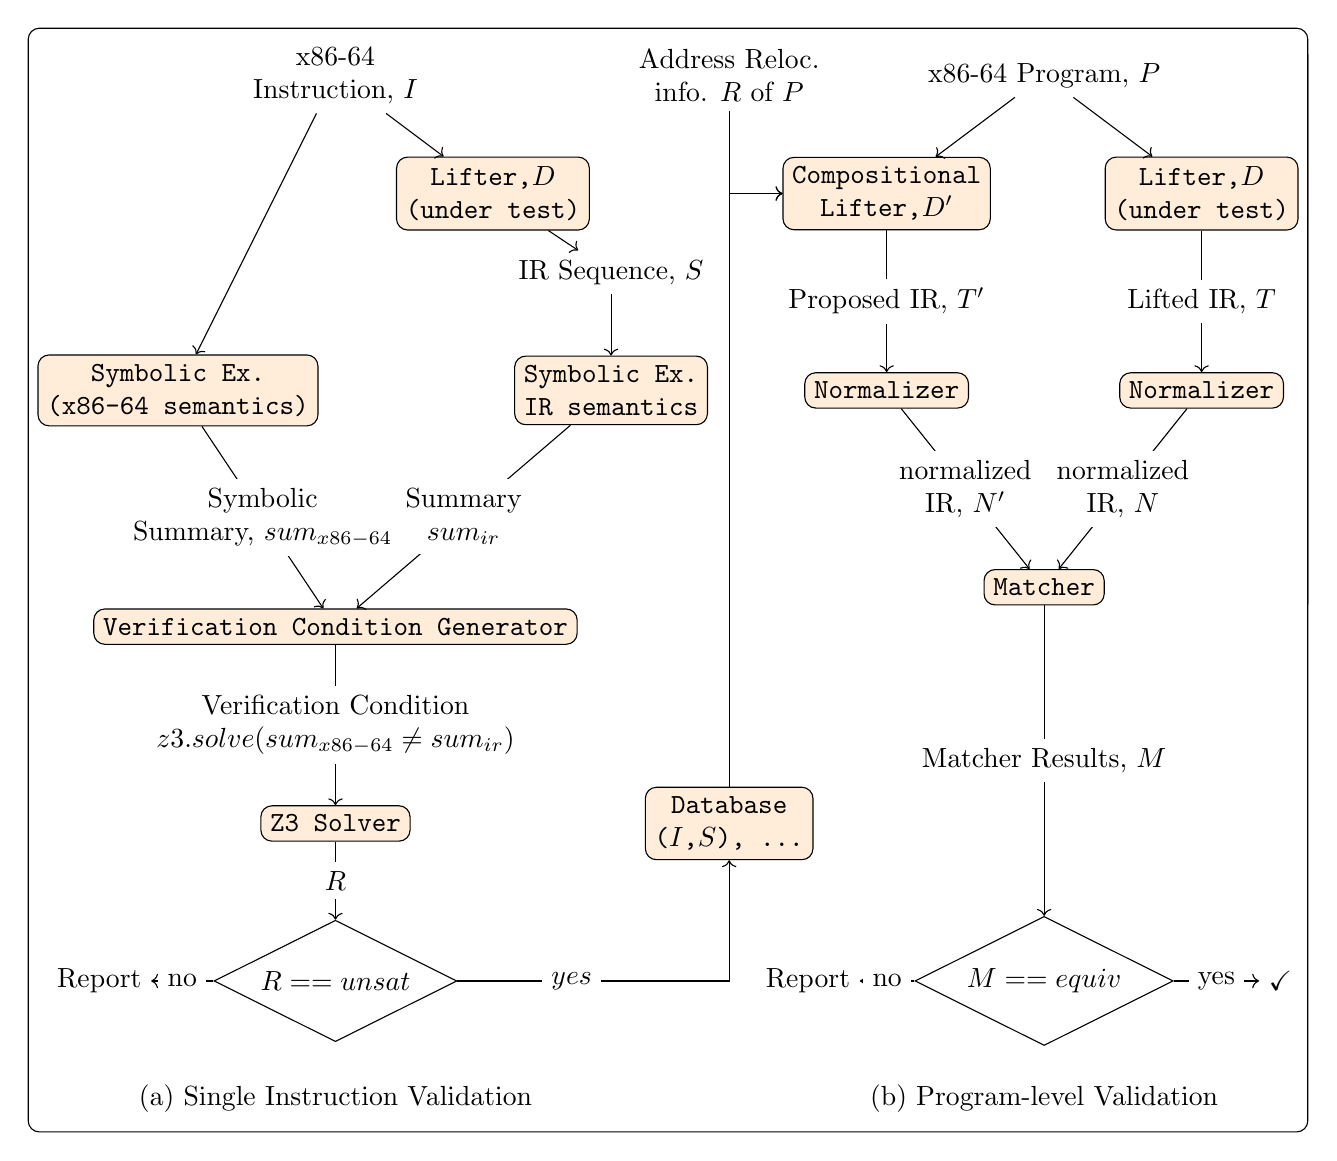
\begin{tikzpicture}[%node distance=2.5cm,
every node/.style={fill=white}, align=center]
\tikzset{%
    %>={Latex[width=2mm,length=2mm]},
    % Specifications for style of nodes:
    base/.style = {rectangle, rounded corners,
         text centered},
    process/.style = {base,  fill=orange!15, font=\ttfamily, draw=black},
    basic box/.style = {
        shape = rectangle,
        align = center,
        draw  = #1,
        %fill  = #1!25,
        rounded corners},
      header node/.style = {
        %Minimum Width = header nodes,
        font          = \strut\Large\ttfamily,
        text depth    = +0pt,
        fill          = white,
        draw},
      header/.style = {%
        inner ysep = +1.5em,
        append after command = {
            \pgfextra{\let\TikZlastnode\tikzlastnode}
            node [header node] (header-\TikZlastnode) at (\TikZlastnode.north) {#1}
            %node [span = (\TikZlastnode)(header-\TikZlastnode)] at (fit bounding box) (h-\TikZlastnode) {}
        }
      },
}
\def\blockhdist{2cm}
\def\blockvdist{1.5cm}
\def\phasehdist{8cm}

%%%%%%%%%%%%%%% PHASE I
\node (instr)          [base]  {\ISA\\ Instruction, $I$};
\node (SIVmcsema)   [process, below of=instr, yshift=-0.5cm, 
xshift=\blockhdist]  {Lifter,$D$\\(under test)};
\node (irseq)          [base,below of=SIVmcsema, xshift=\blockvdist]  {IR 
Sequence, $S$};
\node (instrSymEx)   [process, below of=instr, yshift=-2*\blockvdist, xshift=-\blockhdist] {Symbolic Ex.\\(\ISA semantics) };
\node (irSymEx)   [process, below of=irseq, yshift=-0.5cm] {Symbolic Ex.\\IR semantics};
\node (proofGen)   [process, below of=instr, yshift=-4*\blockvdist] 
{Verification Condition Generator};
\node (solver)   [process, below of=proofGen, yshift=-\blockvdist] {Z3 Solver};
\node (decide1)     [draw, below of=solver, yshift=-1cm, diamond, aspect=2]  {$R == unsat$};
\node (report1)       [left of=decide1, xshift=-\phasehdist/4]  {Report};
\node (caption1)     [below of=solver, yshift=-2.5cm] {(a) Single Instruction
    Validation};

\draw[->]             (instr) -- (SIVmcsema);
\draw[->]             (SIVmcsema) -- (irseq);
\draw[->]     (instr) -- (instrSymEx);
\draw[->]     (irseq) -- (irSymEx);
\draw[->]     (instrSymEx) -- node {Symbolic\\Summary, $sum_{\ISA}$} (proofGen);
\draw[->]     (irSymEx) -- node {Summary\\$sum_{ir}$ } (proofGen);
\draw[->]     (proofGen) -- node {Verification Condition\\$z3.solve(sum_{\ISA} 
\ne 
sum_{ir})$} (solver);
\draw[->]     (solver.south) -- node {$R$} (decide1.north);
\draw[->]     (decide1.west) -- node {no} (report1);

%%%%%% Store
\node (store)     [process, right of=solver, 
xshift=\phasehdist/2]{Database\\({$I$,$S$}), \dots};
\draw[->]       (decide1.east) -| node[xshift=-2cm] {$yes$} (store.south);


%%%%%%%%%%%% PHASE II
\node (start)             [base,right of=instr, 
xshift=\phasehdist]                       {\ISA Program, $P$};
\node (compd)             [process, below of=start, yshift=-0.5cm, 
xshift=-\blockhdist]          {Compositional\\Lifter,$D^\prime$};
\node (mcsema)             [process, below of=start, yshift=-0.5cm, 
xshift=\blockhdist]          {Lifter,$D$\\(under test)};
\node (normalizer1)             [process, below of=compd, yshift=-\blockvdist]   {Normalizer};
\node (normalizer2)         [process, below of=mcsema, yshift=-\blockvdist]   {Normalizer};
\node (matcher)     [process, below of=normalizer2, yshift=-\blockvdist, 
xshift=-\blockhdist]   {Matcher};
\node (decide2)     at (decide1 -| matcher) [draw,  diamond, aspect=2]  {$M == equiv$};
\node (caption2)     at (caption1 -| matcher) {(b) Program-level Validation};
\node (report2)       [left of=decide2, xshift=-\phasehdist/4]  {Report};
\node (fine)       [right of=decide2, xshift=\phasehdist/4]  {\checkmark}; 
 
\draw[->]             (start) -- (compd);
\draw[->]             (start) -- (mcsema);
\draw[->]     (compd) -- node {Proposed IR, $T^\prime$} (normalizer1);
\draw[->]     (mcsema) -- node {Lifted IR, $T$} (normalizer2);
\draw[->]     (normalizer1) -- node {normalized\\IR, $N^\prime$} (matcher);
\draw[->]     (normalizer2) -- node {normalized\\IR, $N$} (matcher);
\draw[->]     (matcher) -- node {Matcher Results, $M$} (decide2);
\draw[->]     (store.north) |-  (compd.west);
\draw[->]     (decide2.west) -- node {no} (report2);
\draw[->]     (decide2.east) -- node {yes} (fine);

%% Reloc info
\node (reloc)             [base,right of=instr, 
xshift=\phasehdist/2]                       {Address Reloc. \\ info. 
$R$ of $P$};
\draw[->]       (reloc.south) |-  (compd.west);

%% Outter box
\begin{scope}[on background layer]
\node[fit = (compd)(mcsema)(start)(matcher), basic box = black,] (Phase1) {};
    \node[fit = (compd)(mcsema)(start)(matcher)(instr)(solver)(irseq)(instrSymEx)(irSymEx)(caption1)(caption2), basic box = black,] (Overview) {};
\end{scope}

\end{tikzpicture}
\caption{Overview diagram of the \tv framework}\label{fig:overview}
\end{figure*}

% \tikzset{
%     database/.style={
%         path picture={
%             \draw (0, 1.5*\database@segmentheight) circle [x radius=\database@radius,y radius=\database@aspectratio*\database@radius];
%             \draw (-\database@radius, 0.5*\database@segmentheight) arc [start angle=180,end angle=360,x radius=\database@radius, y radius=\database@aspectratio*\database@radius];
%             \draw (-\database@radius,-0.5*\database@segmentheight) arc [start angle=180,end angle=360,x radius=\database@radius, y radius=\database@aspectratio*\database@radius];
%             \draw (-\database@radius,1.5*\database@segmentheight) -- ++(0,-3*\database@segmentheight) arc [start angle=180,end angle=360,x radius=\database@radius, y radius=\database@aspectratio*\database@radius] -- ++(0,3*\database@segmentheight);
%         },
%         minimum width=2*\database@radius + \pgflinewidth,
%         minimum height=3*\database@segmentheight + 2*\database@aspectratio*\database@radius + \pgflinewidth,
%     },
%     database segment height/.store in=\database@segmentheight,
%     database radius/.store in=\database@radius,
%     database aspect ratio/.store in=\database@aspectratio,
%     database segment height=0.1cm,
%     database radius=0.25cm,
%     database aspect ratio=0.35,
% }


\section{Single \ISA Instruction Validation}
\section{Preliminaries}
\label{sec:prelim}

In this section, we provide background on various pieces of our work:
(i) The binary lifter under test, McSema, (ii) The formal \ISA semantics, and
(iii) The formal \LLVM semantics.

\paragraph{McSema}\label{par:mcsema} \mcsema~\cite{McSema:Recon14} is the most
mature, well tested, open-source lifter to raise binaries from \ISA
instructions to LLVM bitcode.  At a high-level, \mcsema is split into two
parts: (a) frontend, and (b) backend. The frontend is responsible for parsing,
loading, and disassembling a binary and exports an interface to the backend to
query for the required information, e.g., the defined symbols, sizes of
various binary sections, instruction listings etc. The backend then uses this
information and Remill~\cite{Remill} library to lift the individual
instructions. McSema supports multiple different frontends with IDA Pro being
the most robust, and supported option.

Conceptually, the backend implementation of \mcsema is fairly straightforward:
\mcsema exposes all of architecture state, i.e., the program registers,
conditional flags, and program memory, through an LLVM \emph{struct}, aptly
named \Mcstate. 
Member fields
of the structure correspond to every register (register name, not a physical
register) and flags that can be used during the execution of the program. Instructions
operating on the stack must retrieve the current top of stack from the
appropriate member field (corresponding to \reg{rsp}) in the structure.
\mcsema simply scans through the disassembly of the binary
and lifts each instruction one by one, emitting code to read and update the
members of \emph{state} as defined by the instruction semantics. In essence,
the code lifted by \mcsema simply \emph{simulates} the binary in \LLVM.

%The main idea behind \mcsema lies in the simulation of the original binary,
%which in turns requires architectural state and memory of the target
%processor. There is no explicit stack by default.  To simulate state of the
%processor, an LLVM structure type called \emph{state} is used. Member fields
%of the structure correspond to every register (register name, not a physical
%register) that can be used during the execution of the program. Instructions
%operating on the stack must retrieve the current top of stack from the
%appropriate member field (corresponding to \reg{rsp}) in the structure.
%%\todo[inline]{Unclear: Since structure only holds registers, say which
%%register is used to retrieve "current top of stack."}
%\mcsema  performs decompilation of the binary code by translating the machine
%instructions to operations on this \emph{state} structure, according to the
%machine specification. This lifting process works by translating each assembly
%instruction in the procedure into an IR sequence,  which explicitly specifies
%how it affects the machine's memory and registers, including the flags.
%\paragraph{\ISA \& LLVM formal semantics}
%The present work needs the formal
%semantics of \ISA and LLVM, which we borrowed from~\cite{DasguptaAdve:PLDI19}
%and~\cite{LLVMSEMA} respectively. Both semantics are developed using
%\K~\cite{k-primer-2013-v32}\cmt{\url{http://kframework.org}}, which is a
%framework for defining formal language semantics.

\paragraph{K-Framework}\label{par:k} The presented work needs the formal
semantics of \ISA and LLVM, which we borrowed from~\cite{DasguptaAdve:PLDI19}
and~\cite{LLVMSEMA} respectively (and described next). Both semantics are developed using
\K~\cite{k-primer-2013-v32}\cmt{\url{http://kframework.org}}, which is a
framework for defining formal language semantics. Given a syntax and a
semantics of a language, \K automatically generates a parser, an interpreter, 
a symbolic execution engine, as well as
formal analysis tools such as model checkers and deductive program verifiers,
at no additional effort. Using the interpreter, one can test their
semantics immediately, which significantly increases the efficiency of
semantics developments. Furthermore, the formal analysis tools
facilitate formal reasoning about the given language semantics.  This
helps both the applicability of the semantics and in the
engineering the semantics itself.

\paragraph{\ISA Formal Semantics} Our work uses the state-of-the-art \ISA
semantics developed by Dasgupta et al.~\cite{DasguptaAdve:PLDI19}, which
presents the most complete and thoroughly tested formal semantics of x86-64 to
date, and faithfully formalizes all non-deprecated, sequential
user-level instructions of x86-64 Haswell instruction set architecture.
This totals to 3155 instruction variants, corresponding to 774 mnemonics.
Their semantics are fully executable, and includes a symbolic execution engine
automatically generated by \K framework
%
    \footnote{Given a syntax and a semantics of a language, \K automatically
    generates a parser, an interpreter, a symbolic execution engine, as well
    as formal analysis tools such as model checkers and deductive program
    verifiers, at no additional effort.}.
%

\paragraph{\LLVM Formal Semantics} We use the LLVM formal semantics as defined
in \K~\cite{LLVMSEMA}, which models LLVM types (integers, composite arrays and
structs, corresponding pointers), the \texttt{getelementptr} instruction (used
to compute the address of an element nested within a composite),  integer
arithmetic \& comparison operators, memory operations (\texttt{load},
\texttt{store}, and \texttt{alloca}), control flow instructions for
unconditional and conditional branches, as well as function calls and returns.
However, the semantics does not support: floating point, vector types, and
most LLVM intrinsic functions and therefore we cannot validate the \tv for
such instructions.  This is a limitation of the available LLVM semantics, and
not a limitation of our work.

.
%\todo[inline]{The last 2 sentences are nice, but could be dropped if space is tight.}
%\todo[color=yellow]{These two semantics are two of the most
%    important building blocks. Can we make them top-level paragraphs?}
%\paragraph{\ISA Semantics} \todo{These two semantics are two of the most
%important building blocks. Can we make them top-level paragraphs?}
%The formal model~\cite{DasguptaAdve:PLDI19}
%presents the most complete and thoroughly tested formal semantics of x86-64 to
%date, which faithfully formalizes all the  non-deprecated, sequential
%user-level instructions of the x86-64 Haswell instruction set architecture.
%This totals 3155 instruction variants, corresponding to 774 mnemonics.  The
%semantics is fully executable, and comes with an
%automatically generated symbolic execution engine (thanks to the \K framework),
%which we leverage in this work.
%
%\paragraph{LLVM Semantics} The formal semantics of \LLVM is provided by
%~\cite{LLVMSEMA}, which models  various LLVM types (like integer types,
%    composite array and struct types, the  corresponding pointer types, and the
%    \texttt{getelementptr} instruction used to compute the address of an element nested
%    within a composite type),  integer arithmetic \& comparison operators,
%  memory operations (like \texttt{load}, \texttt{store}, and \texttt{alloca}), 
%  control flow instructions
%  for unconditional and conditional branches, as well as function calls and
%  returns. The current version of the semantics does not support floating point
%  or vector types and most LLVM intrinsic functions, which constrains our experiments
%  but does not affect the overall approach proposed and evaluation in this work.
%  \todo{Check last sentence.}

%\paragraph{Stoke Libraries}\label{par:stoke} Stoke~\cite{Stoke2013} is a
%stochastic superoptimizer and program synthesizer for the x86-64 instruction
%set.  The project comes with many useful libraries to (1) query interesting
%properties of \ISA instructions (like type, size, inputs \& outputs etc.),
%(2) disassemble \ISA programs, and (3) analyze  \ISA programs to infer
%properties related to control- \& data-flow. We make use of these in our
%work.
%
%The rest of this paper is organized as follows: we discuss our \siv
%in~\ref{sec:siv}, and then move on to show how we use the validated sequences of
%IR instructions to construct a \emph{\compd} and use it to for \plv
%in~\ref{sec:plv}. Finally, we show the effectiveness of our developed techniques
%through our evaluation in~\ref{sec:eval}.

\section{\ISA Program-Level Validation}
\subsection{Compositional Decompiler}
\subsection{Normalizer}
\subsection{Matcher}

\chapter{Scalable Validation of Binary Lifters}\label{chap:scalable-val}

Validating the correctness of binary lifters is pivotal to gain trust in
binary analysis, especially when used in scenarios where correctness is
important, e.g., in security analysis, binary patching, or recompilation
to other ISAs. Existing approaches focus on validating the correctness of
lifting a single instruction and do not scale to full programs. In this
work we show that formal translation validation of single instructions for
x86-64 is practical and develop a novel technique that uses validated
instructions to scale to program level validation, thereby eliminating the
bottleneck of heavy-weight equivalence checkers at the program level. Our
work is the first to to do \tv of single instructions on an architecture as 
extensive as \ISA,
uses the most precise formal semantics available, and has the widest
coverage in terms of number of instructions tested for correctness. 
%
To scale to whole programs, our \emph{compositional lifter} composes the validated IR
sequences to create a reference standard. The semantic equivalence check between the
reference and the lifter output is then reduced to a syntactic equivalence check through
use of a normalizer --- a procedure that reduces IR sequences to a
canonical representation.
%    
Using our approach, we find \sivFail new bugs in McSema, a mature open-source
lifter from x86-64 to LLVM IR. For whole programs, our approach was able to
prove equivalence of lifted code for \plvP/\plvT functions taken
from single-source benchmark test-suite.

\chapter{Introduction}\label{sec:ba}

%The problem you want to tackle
Analyzing binary code is crucial in software engineering and security research.
Some of the notable applications of binary analysis can be found in binary
instrumentation
(\cite{Bruening:CGO2003,PEBIL10,Pin:2005,Valgrind:ENTCS03,DynamoRIO:2004}),
  binary translation~\cite{UQBT:2000}, software hardening
  (\cite{Cha:2015,Ford:2008,Zhang,Zhang:2013}), software testing
  (\cite{Chipounov:2011,Avgerinos:2014,godefroid_automated_2008}), CPU
  emulation (\cite{QEMU:USENIX05,Magnusson:2002}), malware detection
  (\cite{Christodorescu:2005,Kruegel:2004,BitBlaze:2008,BAP:CAV11,Egele:USENIX07,Yin:CCS07}),
  automated reverse engineering
  (\cite{Cui:2008,Lin:2008,Schwartz:2013,Yakdan2015NDSS,McSema:Recon14,Angr,Radare2}),
  sand-boxing~\cite{Kiriansky:2002:SEV,Erlingsson:2006,Yee:2009},
  profiling~\cite{Harris:2005,Srivastava:1994}, and automatic exploit
  generation~\cite{Cha:2012}.
               
                 Binary analysis is generally performed by various decompiler
                 projects
                 ~\cite{McSema:Recon14,Remill,Angr1,BAP:CAV11,Radare2}, whose
                 very first step is to translate the machine code to an
                 intermediate representation (IR), and thereby exposing many
                 high-level properties (like control flow, function boundary
                     and prototype, variable and their type etc.) of the
                 binary, which  assist further analysis and/or optimization.
                 Formally establishing faithfulness of the decompilation (i.e.
                     translation from machine code to high level IR) is pivotal
                 to gain trust in any binary analysis. Any bug in the
                 translation would invalidate the binary analysis results.  For
                 example, a malware analysis system might miss vulnerabilities
                 or a binary instrumentation system, instrumenting a buggy IR,
                 might lead to failure or even crash in interpreting the
                 instrumented program. Therefore, automatic validation tools
                 are needed urgently to uncover hidden problems in a binary
                 translator. 

% What is the current state of the art and why that is insufficient
Despite of the importance in establishing the faithfulness of the binary
translators, there has been surprisingly little effort towards that direction.
The most notable approaches are either based on hardware co-simulation
testing~\cite{Martignoni:ISSTA2009,Martignoni:ISSTA2010}, which is limited
because generating specific test-cases to uncover semantic bugs in a lifter is
non-trivial, or differential-testing~\cite{Martignoni:ASPLOS2012,ASE2017},
  which is limited in terms of coverage of the instructions validated and
  faithfulness guarantees it provides (Refer to
      Chapter~\ref{sec:related-work}). 

%How you plan to improve on the state of the art Given the importance  in
%establishing the faithfulness of binary lifter (or translator), 
We propose to employ \tv on binary lifters, as a means to establish the
faithfulness of the translation, by leveraging the semantics of the languages
involved (e.g. the Intel's X86-64 and the high-level IR).  Given the recent
advances in translation validation~\cite{Pnueli:1998} in validating
compilation~\cite{Necula:2000,Pnueli:1998,Stepp:2011,Tristan:2011,VOC2002,TVOC:CAV2005},
  employing \tv to validate binary translators seems a promising direction to
  explore,
%Given the recent advances in translation validation~\cite{Pnueli:1998} in
%validating
%compilation~\cite{Necula:2000,Pnueli:1998,Stepp:2011,Tristan:2011,VOC2002,TVOC:CAV2005},
  %a basic version of this strategy is likely quite feasible today,
  however, there are additional challenges to deal with when it comes to
  validating the decompilation pipeline (Refer Section~\ref{sec:challenges}).
  Moreover, we would like validation approach to be general enough and hence
  applicable to any state-of-the-art binary to high-level IR
  translators~\cite{McSema:Recon14,Remill,FCD,llvm-mctoll,BAP:CAV11,Angr1,DiFederico:CC2017}.
  The idea is to validate the translators without leveraging any knowledge of
  the translation involved, which in turn makes the problem even more
  challenging (Refer Chapter~\ref{sec:future}).
  %thereby avoiding any translator specific customization during validation
  %(Refer Chapter~\ref{sec:future}).  However, having this goal makes the
  %problem even more challenging.

We believe that formally validating the translation is more robust as compared
to (1) validating the translation using random (or low coverage) test-cases,
   and (2) differential testing technique which tests the correctness of a
   translation, generated by a translator, by comparing its behaviors with that
   provided by other translators under test. \cmt{This means, declaring a
     translation to be correct assumes the correctness of all the translator.}

%Summarize your contributions
\paragraph{Contributions}
Below we propose the  primary contributions of our work.

\textbf{\emph{Most Complete user-level \ISA Semantics:}} Towards the goals of
\tv of binary translators, we developed\cite{DasguptaAdve:PLDI19} the most
complete and thoroughly tested formal semantics of \ISA to date, which
faithfully formalizes all the non-deprecated, sequential user-level
instructions of the x86-64 Haswell instruction set architecture. 

\textbf{\emph{Translation validation on binary translators~}} We propose tools
and techniques to formally validate the translation from binary to high level
IR.  To the best of our knowledge, we are the first to propose \tv to establish
the faithfulness of binary lifters targeting LLVM as their high-level IR. We
would demonstrate the applicability of our approach by validating the
translation of a realistic decompiler, McSema~\cite{McSema:Recon14}.
%and revng~\cite{DiFederico:CC2017}}.

\textbf{\emph{Automated back-box approaches to \tv~}} We would like our
technique to work automatically and uniformly across translators considering
the translators as black-boxes, i.e. without using any translator-generated
hints  or translator-specific heuristics to assist the validation. We would
like to demonstrate the effectiveness  of our solution by validating against
two or more decompilers.  Optionally, we would like to use machine learning
techniques to infer the  variable or basic block correspondence between binary
and LLVM IR code which will help in realizing a translator-agnostic approach to
\tv.

%\textbf{\emph{Translator-agnostic solution~}}     

%In the next section, we elaborate on our motivation to establish faithfulness
%of binary translators.  Why it is important \section{Benefits of Binary
  %Analysis}

\section{Approach Overview}
\label{sec:Approach}

\makeatletter
\makeatother

\begin{figure*}
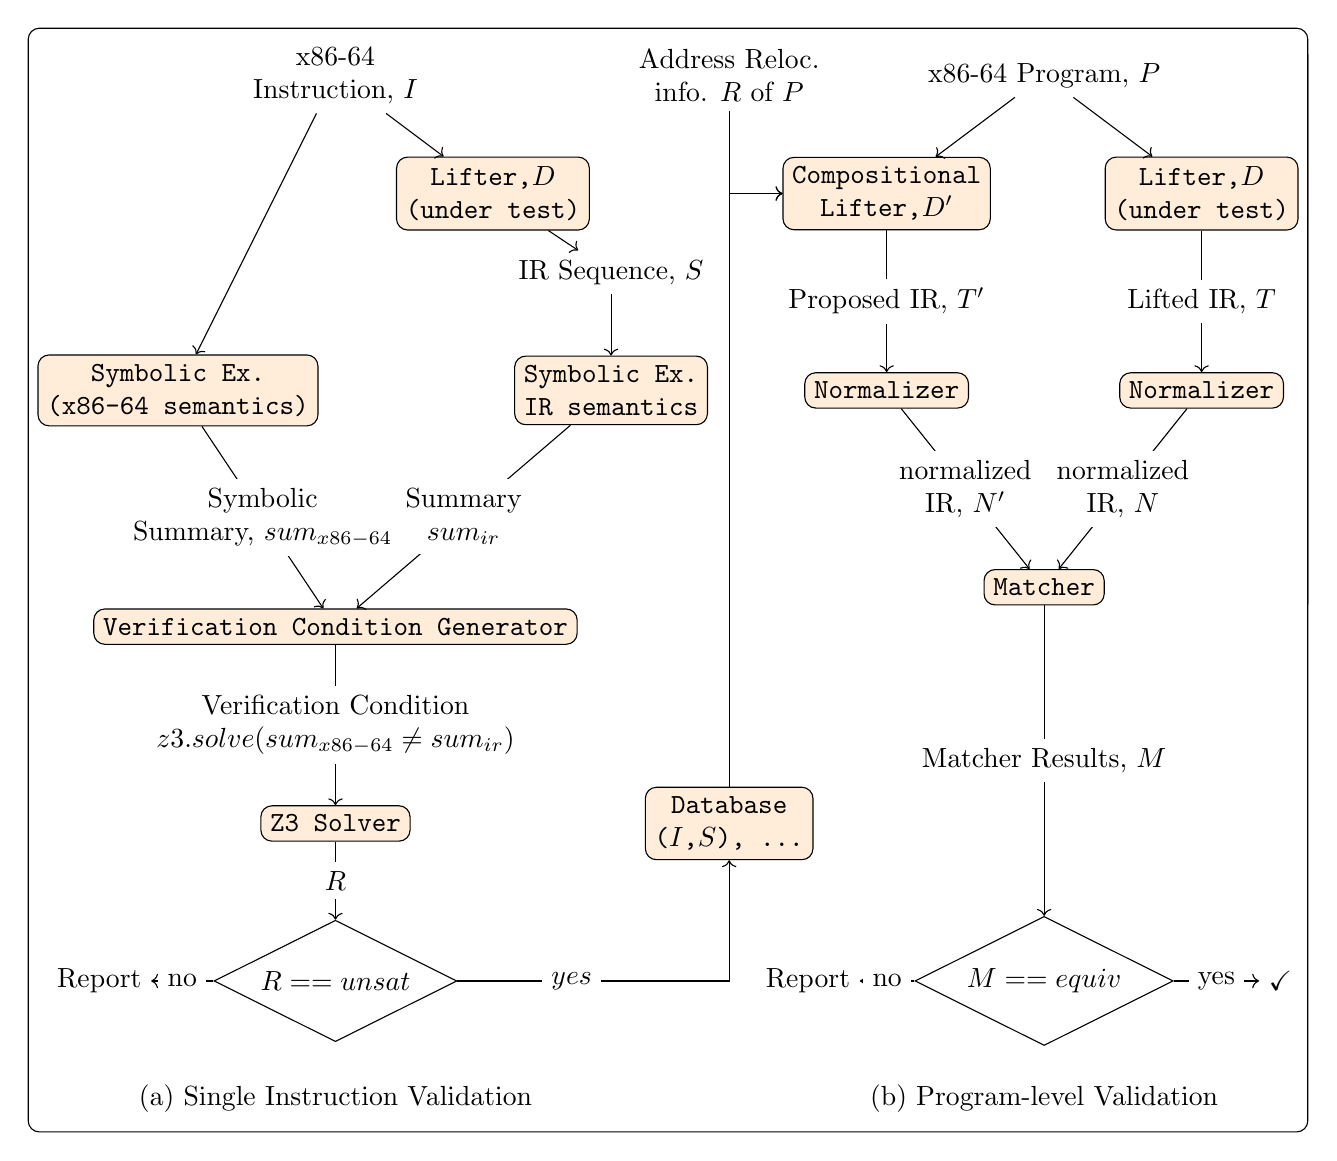
\begin{tikzpicture}[%node distance=2.5cm,
every node/.style={fill=white}, align=center]
\tikzset{%
    %>={Latex[width=2mm,length=2mm]},
    % Specifications for style of nodes:
    base/.style = {rectangle, rounded corners,
         text centered},
    process/.style = {base,  fill=orange!15, font=\ttfamily, draw=black},
    basic box/.style = {
        shape = rectangle,
        align = center,
        draw  = #1,
        %fill  = #1!25,
        rounded corners},
      header node/.style = {
        %Minimum Width = header nodes,
        font          = \strut\Large\ttfamily,
        text depth    = +0pt,
        fill          = white,
        draw},
      header/.style = {%
        inner ysep = +1.5em,
        append after command = {
            \pgfextra{\let\TikZlastnode\tikzlastnode}
            node [header node] (header-\TikZlastnode) at (\TikZlastnode.north) {#1}
            %node [span = (\TikZlastnode)(header-\TikZlastnode)] at (fit bounding box) (h-\TikZlastnode) {}
        }
      },
}
\def\blockhdist{2cm}
\def\blockvdist{1.5cm}
\def\phasehdist{8cm}

%%%%%%%%%%%%%%% PHASE I
\node (instr)          [base]  {\ISA\\ Instruction, $I$};
\node (SIVmcsema)   [process, below of=instr, yshift=-0.5cm, 
xshift=\blockhdist]  {Lifter,$D$\\(under test)};
\node (irseq)          [base,below of=SIVmcsema, xshift=\blockvdist]  {IR 
Sequence, $S$};
\node (instrSymEx)   [process, below of=instr, yshift=-2*\blockvdist, xshift=-\blockhdist] {Symbolic Ex.\\(\ISA semantics) };
\node (irSymEx)   [process, below of=irseq, yshift=-0.5cm] {Symbolic Ex.\\IR semantics};
\node (proofGen)   [process, below of=instr, yshift=-4*\blockvdist] 
{Verification Condition Generator};
\node (solver)   [process, below of=proofGen, yshift=-\blockvdist] {Z3 Solver};
\node (decide1)     [draw, below of=solver, yshift=-1cm, diamond, aspect=2]  {$R == unsat$};
\node (report1)       [left of=decide1, xshift=-\phasehdist/4]  {Report};
\node (caption1)     [below of=solver, yshift=-2.5cm] {(a) Single Instruction
    Validation};

\draw[->]             (instr) -- (SIVmcsema);
\draw[->]             (SIVmcsema) -- (irseq);
\draw[->]     (instr) -- (instrSymEx);
\draw[->]     (irseq) -- (irSymEx);
\draw[->]     (instrSymEx) -- node {Symbolic\\Summary, $sum_{\ISA}$} (proofGen);
\draw[->]     (irSymEx) -- node {Summary\\$sum_{ir}$ } (proofGen);
\draw[->]     (proofGen) -- node {Verification Condition\\$z3.solve(sum_{\ISA} 
\ne 
sum_{ir})$} (solver);
\draw[->]     (solver.south) -- node {$R$} (decide1.north);
\draw[->]     (decide1.west) -- node {no} (report1);

%%%%%% Store
\node (store)     [process, right of=solver, 
xshift=\phasehdist/2]{Database\\({$I$,$S$}), \dots};
\draw[->]       (decide1.east) -| node[xshift=-2cm] {$yes$} (store.south);


%%%%%%%%%%%% PHASE II
\node (start)             [base,right of=instr, 
xshift=\phasehdist]                       {\ISA Program, $P$};
\node (compd)             [process, below of=start, yshift=-0.5cm, 
xshift=-\blockhdist]          {Compositional\\Lifter,$D^\prime$};
\node (mcsema)             [process, below of=start, yshift=-0.5cm, 
xshift=\blockhdist]          {Lifter,$D$\\(under test)};
\node (normalizer1)             [process, below of=compd, yshift=-\blockvdist]   {Normalizer};
\node (normalizer2)         [process, below of=mcsema, yshift=-\blockvdist]   {Normalizer};
\node (matcher)     [process, below of=normalizer2, yshift=-\blockvdist, 
xshift=-\blockhdist]   {Matcher};
\node (decide2)     at (decide1 -| matcher) [draw,  diamond, aspect=2]  {$M == equiv$};
\node (caption2)     at (caption1 -| matcher) {(b) Program-level Validation};
\node (report2)       [left of=decide2, xshift=-\phasehdist/4]  {Report};
\node (fine)       [right of=decide2, xshift=\phasehdist/4]  {\checkmark}; 
 
\draw[->]             (start) -- (compd);
\draw[->]             (start) -- (mcsema);
\draw[->]     (compd) -- node {Proposed IR, $T^\prime$} (normalizer1);
\draw[->]     (mcsema) -- node {Lifted IR, $T$} (normalizer2);
\draw[->]     (normalizer1) -- node {normalized\\IR, $N^\prime$} (matcher);
\draw[->]     (normalizer2) -- node {normalized\\IR, $N$} (matcher);
\draw[->]     (matcher) -- node {Matcher Results, $M$} (decide2);
\draw[->]     (store.north) |-  (compd.west);
\draw[->]     (decide2.west) -- node {no} (report2);
\draw[->]     (decide2.east) -- node {yes} (fine);

%% Reloc info
\node (reloc)             [base,right of=instr, 
xshift=\phasehdist/2]                       {Address Reloc. \\ info. 
$R$ of $P$};
\draw[->]       (reloc.south) |-  (compd.west);

%% Outter box
\begin{scope}[on background layer]
\node[fit = (compd)(mcsema)(start)(matcher), basic box = black,] (Phase1) {};
    \node[fit = (compd)(mcsema)(start)(matcher)(instr)(solver)(irseq)(instrSymEx)(irSymEx)(caption1)(caption2), basic box = black,] (Overview) {};
\end{scope}

\end{tikzpicture}
\caption{Overview diagram of the \tv framework}\label{fig:overview}
\end{figure*}

% \tikzset{
%     database/.style={
%         path picture={
%             \draw (0, 1.5*\database@segmentheight) circle [x radius=\database@radius,y radius=\database@aspectratio*\database@radius];
%             \draw (-\database@radius, 0.5*\database@segmentheight) arc [start angle=180,end angle=360,x radius=\database@radius, y radius=\database@aspectratio*\database@radius];
%             \draw (-\database@radius,-0.5*\database@segmentheight) arc [start angle=180,end angle=360,x radius=\database@radius, y radius=\database@aspectratio*\database@radius];
%             \draw (-\database@radius,1.5*\database@segmentheight) -- ++(0,-3*\database@segmentheight) arc [start angle=180,end angle=360,x radius=\database@radius, y radius=\database@aspectratio*\database@radius] -- ++(0,3*\database@segmentheight);
%         },
%         minimum width=2*\database@radius + \pgflinewidth,
%         minimum height=3*\database@segmentheight + 2*\database@aspectratio*\database@radius + \pgflinewidth,
%     },
%     database segment height/.store in=\database@segmentheight,
%     database radius/.store in=\database@radius,
%     database aspect ratio/.store in=\database@aspectratio,
%     database segment height=0.1cm,
%     database radius=0.25cm,
%     database aspect ratio=0.35,
% }


\section{Single \ISA Instruction Validation}
\section{Preliminaries}
\label{sec:prelim}

In this section, we provide background on various pieces of our work:
(i) The binary lifter under test, McSema, (ii) The formal \ISA semantics, and
(iii) The formal \LLVM semantics.

\paragraph{McSema}\label{par:mcsema} \mcsema~\cite{McSema:Recon14} is the most
mature, well tested, open-source lifter to raise binaries from \ISA
instructions to LLVM bitcode.  At a high-level, \mcsema is split into two
parts: (a) frontend, and (b) backend. The frontend is responsible for parsing,
loading, and disassembling a binary and exports an interface to the backend to
query for the required information, e.g., the defined symbols, sizes of
various binary sections, instruction listings etc. The backend then uses this
information and Remill~\cite{Remill} library to lift the individual
instructions. McSema supports multiple different frontends with IDA Pro being
the most robust, and supported option.

Conceptually, the backend implementation of \mcsema is fairly straightforward:
\mcsema exposes all of architecture state, i.e., the program registers,
conditional flags, and program memory, through an LLVM \emph{struct}, aptly
named \Mcstate. 
Member fields
of the structure correspond to every register (register name, not a physical
register) and flags that can be used during the execution of the program. Instructions
operating on the stack must retrieve the current top of stack from the
appropriate member field (corresponding to \reg{rsp}) in the structure.
\mcsema simply scans through the disassembly of the binary
and lifts each instruction one by one, emitting code to read and update the
members of \emph{state} as defined by the instruction semantics. In essence,
the code lifted by \mcsema simply \emph{simulates} the binary in \LLVM.

%The main idea behind \mcsema lies in the simulation of the original binary,
%which in turns requires architectural state and memory of the target
%processor. There is no explicit stack by default.  To simulate state of the
%processor, an LLVM structure type called \emph{state} is used. Member fields
%of the structure correspond to every register (register name, not a physical
%register) that can be used during the execution of the program. Instructions
%operating on the stack must retrieve the current top of stack from the
%appropriate member field (corresponding to \reg{rsp}) in the structure.
%%\todo[inline]{Unclear: Since structure only holds registers, say which
%%register is used to retrieve "current top of stack."}
%\mcsema  performs decompilation of the binary code by translating the machine
%instructions to operations on this \emph{state} structure, according to the
%machine specification. This lifting process works by translating each assembly
%instruction in the procedure into an IR sequence,  which explicitly specifies
%how it affects the machine's memory and registers, including the flags.
%\paragraph{\ISA \& LLVM formal semantics}
%The present work needs the formal
%semantics of \ISA and LLVM, which we borrowed from~\cite{DasguptaAdve:PLDI19}
%and~\cite{LLVMSEMA} respectively. Both semantics are developed using
%\K~\cite{k-primer-2013-v32}\cmt{\url{http://kframework.org}}, which is a
%framework for defining formal language semantics.

\paragraph{K-Framework}\label{par:k} The presented work needs the formal
semantics of \ISA and LLVM, which we borrowed from~\cite{DasguptaAdve:PLDI19}
and~\cite{LLVMSEMA} respectively (and described next). Both semantics are developed using
\K~\cite{k-primer-2013-v32}\cmt{\url{http://kframework.org}}, which is a
framework for defining formal language semantics. Given a syntax and a
semantics of a language, \K automatically generates a parser, an interpreter, 
a symbolic execution engine, as well as
formal analysis tools such as model checkers and deductive program verifiers,
at no additional effort. Using the interpreter, one can test their
semantics immediately, which significantly increases the efficiency of
semantics developments. Furthermore, the formal analysis tools
facilitate formal reasoning about the given language semantics.  This
helps both the applicability of the semantics and in the
engineering the semantics itself.

\paragraph{\ISA Formal Semantics} Our work uses the state-of-the-art \ISA
semantics developed by Dasgupta et al.~\cite{DasguptaAdve:PLDI19}, which
presents the most complete and thoroughly tested formal semantics of x86-64 to
date, and faithfully formalizes all non-deprecated, sequential
user-level instructions of x86-64 Haswell instruction set architecture.
This totals to 3155 instruction variants, corresponding to 774 mnemonics.
Their semantics are fully executable, and includes a symbolic execution engine
automatically generated by \K framework
%
    \footnote{Given a syntax and a semantics of a language, \K automatically
    generates a parser, an interpreter, a symbolic execution engine, as well
    as formal analysis tools such as model checkers and deductive program
    verifiers, at no additional effort.}.
%

\paragraph{\LLVM Formal Semantics} We use the LLVM formal semantics as defined
in \K~\cite{LLVMSEMA}, which models LLVM types (integers, composite arrays and
structs, corresponding pointers), the \texttt{getelementptr} instruction (used
to compute the address of an element nested within a composite),  integer
arithmetic \& comparison operators, memory operations (\texttt{load},
\texttt{store}, and \texttt{alloca}), control flow instructions for
unconditional and conditional branches, as well as function calls and returns.
However, the semantics does not support: floating point, vector types, and
most LLVM intrinsic functions and therefore we cannot validate the \tv for
such instructions.  This is a limitation of the available LLVM semantics, and
not a limitation of our work.

.
%\todo[inline]{The last 2 sentences are nice, but could be dropped if space is tight.}
%\todo[color=yellow]{These two semantics are two of the most
%    important building blocks. Can we make them top-level paragraphs?}
%\paragraph{\ISA Semantics} \todo{These two semantics are two of the most
%important building blocks. Can we make them top-level paragraphs?}
%The formal model~\cite{DasguptaAdve:PLDI19}
%presents the most complete and thoroughly tested formal semantics of x86-64 to
%date, which faithfully formalizes all the  non-deprecated, sequential
%user-level instructions of the x86-64 Haswell instruction set architecture.
%This totals 3155 instruction variants, corresponding to 774 mnemonics.  The
%semantics is fully executable, and comes with an
%automatically generated symbolic execution engine (thanks to the \K framework),
%which we leverage in this work.
%
%\paragraph{LLVM Semantics} The formal semantics of \LLVM is provided by
%~\cite{LLVMSEMA}, which models  various LLVM types (like integer types,
%    composite array and struct types, the  corresponding pointer types, and the
%    \texttt{getelementptr} instruction used to compute the address of an element nested
%    within a composite type),  integer arithmetic \& comparison operators,
%  memory operations (like \texttt{load}, \texttt{store}, and \texttt{alloca}), 
%  control flow instructions
%  for unconditional and conditional branches, as well as function calls and
%  returns. The current version of the semantics does not support floating point
%  or vector types and most LLVM intrinsic functions, which constrains our experiments
%  but does not affect the overall approach proposed and evaluation in this work.
%  \todo{Check last sentence.}

%\paragraph{Stoke Libraries}\label{par:stoke} Stoke~\cite{Stoke2013} is a
%stochastic superoptimizer and program synthesizer for the x86-64 instruction
%set.  The project comes with many useful libraries to (1) query interesting
%properties of \ISA instructions (like type, size, inputs \& outputs etc.),
%(2) disassemble \ISA programs, and (3) analyze  \ISA programs to infer
%properties related to control- \& data-flow. We make use of these in our
%work.
%
%The rest of this paper is organized as follows: we discuss our \siv
%in~\ref{sec:siv}, and then move on to show how we use the validated sequences of
%IR instructions to construct a \emph{\compd} and use it to for \plv
%in~\ref{sec:plv}. Finally, we show the effectiveness of our developed techniques
%through our evaluation in~\ref{sec:eval}.

\section{\ISA Program-Level Validation}
\subsection{Compositional Decompiler}
\subsection{Normalizer}
\subsection{Matcher}

\section{Preliminaries}
\label{sec:prelim}

In this section, we provide background on various pieces of our work:
(i) The binary lifter under test, McSema, (ii) The formal \ISA semantics, and
(iii) The formal \LLVM semantics.

\paragraph{McSema}\label{par:mcsema} \mcsema~\cite{McSema:Recon14} is the most
mature, well tested, open-source lifter to raise binaries from \ISA
instructions to LLVM bitcode.  At a high-level, \mcsema is split into two
parts: (a) frontend, and (b) backend. The frontend is responsible for parsing,
loading, and disassembling a binary and exports an interface to the backend to
query for the required information, e.g., the defined symbols, sizes of
various binary sections, instruction listings etc. The backend then uses this
information and Remill~\cite{Remill} library to lift the individual
instructions. McSema supports multiple different frontends with IDA Pro being
the most robust, and supported option.

Conceptually, the backend implementation of \mcsema is fairly straightforward:
\mcsema exposes all of architecture state, i.e., the program registers,
conditional flags, and program memory, through an LLVM \emph{struct}, aptly
named \Mcstate. 
Member fields
of the structure correspond to every register (register name, not a physical
register) and flags that can be used during the execution of the program. Instructions
operating on the stack must retrieve the current top of stack from the
appropriate member field (corresponding to \reg{rsp}) in the structure.
\mcsema simply scans through the disassembly of the binary
and lifts each instruction one by one, emitting code to read and update the
members of \emph{state} as defined by the instruction semantics. In essence,
the code lifted by \mcsema simply \emph{simulates} the binary in \LLVM.

%The main idea behind \mcsema lies in the simulation of the original binary,
%which in turns requires architectural state and memory of the target
%processor. There is no explicit stack by default.  To simulate state of the
%processor, an LLVM structure type called \emph{state} is used. Member fields
%of the structure correspond to every register (register name, not a physical
%register) that can be used during the execution of the program. Instructions
%operating on the stack must retrieve the current top of stack from the
%appropriate member field (corresponding to \reg{rsp}) in the structure.
%%\todo[inline]{Unclear: Since structure only holds registers, say which
%%register is used to retrieve "current top of stack."}
%\mcsema  performs decompilation of the binary code by translating the machine
%instructions to operations on this \emph{state} structure, according to the
%machine specification. This lifting process works by translating each assembly
%instruction in the procedure into an IR sequence,  which explicitly specifies
%how it affects the machine's memory and registers, including the flags.
%\paragraph{\ISA \& LLVM formal semantics}
%The present work needs the formal
%semantics of \ISA and LLVM, which we borrowed from~\cite{DasguptaAdve:PLDI19}
%and~\cite{LLVMSEMA} respectively. Both semantics are developed using
%\K~\cite{k-primer-2013-v32}\cmt{\url{http://kframework.org}}, which is a
%framework for defining formal language semantics.

\paragraph{K-Framework}\label{par:k} The presented work needs the formal
semantics of \ISA and LLVM, which we borrowed from~\cite{DasguptaAdve:PLDI19}
and~\cite{LLVMSEMA} respectively (and described next). Both semantics are developed using
\K~\cite{k-primer-2013-v32}\cmt{\url{http://kframework.org}}, which is a
framework for defining formal language semantics. Given a syntax and a
semantics of a language, \K automatically generates a parser, an interpreter, 
a symbolic execution engine, as well as
formal analysis tools such as model checkers and deductive program verifiers,
at no additional effort. Using the interpreter, one can test their
semantics immediately, which significantly increases the efficiency of
semantics developments. Furthermore, the formal analysis tools
facilitate formal reasoning about the given language semantics.  This
helps both the applicability of the semantics and in the
engineering the semantics itself.

\paragraph{\ISA Formal Semantics} Our work uses the state-of-the-art \ISA
semantics developed by Dasgupta et al.~\cite{DasguptaAdve:PLDI19}, which
presents the most complete and thoroughly tested formal semantics of x86-64 to
date, and faithfully formalizes all non-deprecated, sequential
user-level instructions of x86-64 Haswell instruction set architecture.
This totals to 3155 instruction variants, corresponding to 774 mnemonics.
Their semantics are fully executable, and includes a symbolic execution engine
automatically generated by \K framework
%
    \footnote{Given a syntax and a semantics of a language, \K automatically
    generates a parser, an interpreter, a symbolic execution engine, as well
    as formal analysis tools such as model checkers and deductive program
    verifiers, at no additional effort.}.
%

\paragraph{\LLVM Formal Semantics} We use the LLVM formal semantics as defined
in \K~\cite{LLVMSEMA}, which models LLVM types (integers, composite arrays and
structs, corresponding pointers), the \texttt{getelementptr} instruction (used
to compute the address of an element nested within a composite),  integer
arithmetic \& comparison operators, memory operations (\texttt{load},
\texttt{store}, and \texttt{alloca}), control flow instructions for
unconditional and conditional branches, as well as function calls and returns.
However, the semantics does not support: floating point, vector types, and
most LLVM intrinsic functions and therefore we cannot validate the \tv for
such instructions.  This is a limitation of the available LLVM semantics, and
not a limitation of our work.

.
%\todo[inline]{The last 2 sentences are nice, but could be dropped if space is tight.}
%\todo[color=yellow]{These two semantics are two of the most
%    important building blocks. Can we make them top-level paragraphs?}
%\paragraph{\ISA Semantics} \todo{These two semantics are two of the most
%important building blocks. Can we make them top-level paragraphs?}
%The formal model~\cite{DasguptaAdve:PLDI19}
%presents the most complete and thoroughly tested formal semantics of x86-64 to
%date, which faithfully formalizes all the  non-deprecated, sequential
%user-level instructions of the x86-64 Haswell instruction set architecture.
%This totals 3155 instruction variants, corresponding to 774 mnemonics.  The
%semantics is fully executable, and comes with an
%automatically generated symbolic execution engine (thanks to the \K framework),
%which we leverage in this work.
%
%\paragraph{LLVM Semantics} The formal semantics of \LLVM is provided by
%~\cite{LLVMSEMA}, which models  various LLVM types (like integer types,
%    composite array and struct types, the  corresponding pointer types, and the
%    \texttt{getelementptr} instruction used to compute the address of an element nested
%    within a composite type),  integer arithmetic \& comparison operators,
%  memory operations (like \texttt{load}, \texttt{store}, and \texttt{alloca}), 
%  control flow instructions
%  for unconditional and conditional branches, as well as function calls and
%  returns. The current version of the semantics does not support floating point
%  or vector types and most LLVM intrinsic functions, which constrains our experiments
%  but does not affect the overall approach proposed and evaluation in this work.
%  \todo{Check last sentence.}

%\paragraph{Stoke Libraries}\label{par:stoke} Stoke~\cite{Stoke2013} is a
%stochastic superoptimizer and program synthesizer for the x86-64 instruction
%set.  The project comes with many useful libraries to (1) query interesting
%properties of \ISA instructions (like type, size, inputs \& outputs etc.),
%(2) disassemble \ISA programs, and (3) analyze  \ISA programs to infer
%properties related to control- \& data-flow. We make use of these in our
%work.
%
%The rest of this paper is organized as follows: we discuss our \siv
%in~\ref{sec:siv}, and then move on to show how we use the validated sequences of
%IR instructions to construct a \emph{\compd} and use it to for \plv
%in~\ref{sec:plv}. Finally, we show the effectiveness of our developed techniques
%through our evaluation in~\ref{sec:eval}.

\section{Single Instruction Validation}\label{sec:siv}

The \siv is responsible for validating the lifting (using McSema) of an \ISA 
instruction \s{I} to \LLVM sequence \s{S}. This is achieved by (1) 
%Identifying the input/output variables for \s{I} and \s{S} and 
Establishing variable correspondence between \s{I} and \s{S}, (2) Generating 
symbolic summaries 
individually for \s{I} and \s{S} for each output variable, (3) Generating 
verification conditions meant to establish semantic equivalence between the 
corresponding pair of summaries, and solving those using an SMT solver (\Z). 
Next, we describe each one of these steps.

\paragraph{(1) Establishing variable correspondence:}   
%First, we need to identify the input/output variables of an \ISA instruction 
%and the corresponding lifted IR sequence. For each \ISA instruction, this 
%information is ready accessible using Stoke libraries to determine what are 
%the 
%implicit and explicit 
%register/memory/flags which are read or written by the instruction.
``Variable correspondence'' between \s{I} and \s{S} refers to identifying the 
correspondence between the input/output variables of \s{I}\footnote{By 
input/output variables of an instruction we mean implicit and explicit 
    register/memory/flags which are read or written.} and the 
    virtual registers in 
\s{S}. As described in Section~\ref{par:mcsema}, \mcsema uses a \Mcstate 
structure to
model the architecture state, which holds all the simulated architectural
registers at different offsets of the structure.\footnote{Another decompiler,
  fcd~\cite{FCD}, also has the similar approach of modeling.
    Rev.Ng~\cite{DiFederico:CC2017} models the architecture registers as LLVM
    globals.}  Hence, the input and output variables in the context of
    \mcsema are particular \emph{struct} fields, identified by constant offsets.
%
 As an example, for an instruction \instr{adcq \%rax, \%rbx}, the input variables are
 \reg{cf}, \reg{rax} \& \reg{rbx}, and output variables are \reg{rbx}, \reg{cf},
 \reg{pf}, \reg{sf}, \reg{zf}, \reg{of} and \reg{af}. 
The following shows how
 these input/output registers are mapped to the \mcsema \Mcstate structure.

\begin{lstlisting}[style=KRULE]
// State structure type (irrelevant fields shown as ...)
%struct.State (*$\mapsto$*) type { %struct.ArchState, ..., 
    %struct.ArithFlags,..., ..., ..., %struct.GPR, ...}

// Pointers to simulated registers are accessed as below
getelementptr inbounds %struct.State, %struct.State* 
    %state, i64 0, i32 (*\textbf{m}*), i32 (*\textbf{n}*), i32 0, i32 0

// Mapping of various simulated registers to getelementptr offsets
    rax (*$\mapsto$*) m = 6  n = 1;  rbx (*$\mapsto$*) m = 6  n = 3
     cf (*$\mapsto$*) m = 1  n = 1;   pf (*$\mapsto$*) m = 1  n = 3
     af (*$\mapsto$*) m = 1  n = 5;   zf (*$\mapsto$*) m = 1  n = 7
     sf (*$\mapsto$*) m = 1  n = 9;   of (*$\mapsto$*) m = 1  n = 13
\end{lstlisting}

We use the above architectural state representation of \mcsema to infer the
``variable correspondence'' between the \ISA instruction and its corresponding
lifted IR sequence\footnote{Similar inference
    for fcd~\cite{FCD}. For Rev.Ng~\cite{DiFederico:CC2017}, ``variable
    correspondence''  refers to  mapping between the \ISA registers and the
    LLVM globals}.

\cmt{  
For \mcsema, the ``variable correspondence''  means identifying the one-on-one
mapping between the \ISA registers and the \emph{struct} offsets.
%
\footnote{Same
  with fcd~\cite{FCD}. For Rev.Ng~\cite{DiFederico:CC2017}, ``variable
    correspondence''  refers to  mapping between the \ISA registers and the
    LLVM globals},}
%
% which is a trivial task once the input/output variable are already identified.
%
%\todo[inline,color=yellow]{I think we should use "variable correspondence" to 
%mean the mapping
%of operands of I to operands of S for each I in the input program. The mapping 
%above 
%is an architectural state representation, not a variable correspondence.  Your 
%%%tools 
%use the knowledge of the
%latter to extract the former automatically for each I.  Need to add a brief 
%paragraph here to describe that.}

%One may very rightfully think that it may not be easy or scalable to look into 
%the 
%implementation details of an arbitrary decompiler to collect such information. 
%To avoid that we developed an automated tool which will collect the such 
%variable correspondence information. The idea is to feed carefully selected 
%\ISA instructions to the  
 
\paragraph{(2) Generating symbolic summaries:}
The \K framework takes the formal semantics of \ISA and \LLVM and generates 
symbolic execution engines automatically, which we leverage to do 
symbolic execution of an \ISA instruction and the corresponding lifted \LLVM sequence 
individually. Before symbolic execution, we assign symbolic values to the input 
variables to obtain a summary over those. For the running example of 
\instr{adcq, \%rax, \%rbx}, the following shows the symbolic summary for just the 
output register \reg{rbx}\footnote{All the values or
    addresses, stored in registers, memory or
    flags, are represented as bit-vectors which are depicted in
    this paper as $V_W$ and interpreted as a bit-vector of size $W$
    and value $V$.}. 

\vspace{45pt}
%\todo[inline,color=yellow]{Usual notation is with a footnote: $V_W$. You could 
%use footnotes
%in formatted text and use W.V in the listings.  W.V makes the listing
%below very cluttered, though: wish there was a better choice.}

%\begin{minipage}{\linewidth}
%\vspace{10pt}
\begin{lstlisting}[style=KRULE]
// VX_CF, VX_RAX and VX_RBX are the symbolic values
// assigned to input variables.
extract ( 
    add ( 
        (#if eq ( VX_CF(*$_1$*) , (*$1_1$*) ) #then 
            add ( concat ( 0(*$_1$*) , VX_RAX(*$_{64}$*) ) , 1(*$_{65}$*) ) 
        #else 
            concat ( 0(*$_1$*) , VX_RAX(*$_{64}$*) ) 
        #fi)
        , concat ( 0(*$_1$*) , VX_RBX(*$_{64}$*)) 
        ) 
    , 1 , 65 ) 
\end{lstlisting}
%\end{minipage}

Similar symbolic summaries will be obtained for
 every simulated register in the lifter IR sequence,
which is omitted for brevity.

%%
\cmt{and 
(3) The fact that x86-64 ISA is largely stable and changes slowly
over time, we can keep a database of \emph{most} of the (\ISA
instruction,
validated IR sequence) pairs computed offline, but one-time, and
the phase two, on the other hand, can use the database for
composition.  Some
instructions variants like immediate, memory and control-flow cannot
be stored before-hand because it is impractical to compute the IR
sequence for all possible constant values. In these case, the IR
sequence can either be generalized from similar instances already
populated in the database or generated afresh and validated on the fly.}

The \ISA ISA includes instructions with Repeat String Operation 
Prefix (e.g. \instr{rep}, \instr{repz} etc.) to repeat a string instruction the 
number of times specified in the 
count register or until the indicated condition by the prefix is no longer met.
That is, their specification involves a loop which the symbolic 
execution must handle. We address this by symbolically executing those 
instruction with symbolic input state and comparing the summaries (using 
solver checks) of any single $i^{th}$ iteration of the two loops. This suffices 
to establish equivalence between the two loops, by coinductive 
reasoning~\cite{bisimulations} and the fact that such loops are bounded by a 
constant thus must terminate.

%\todo{"Capturing core behaviors" is not enough for soundness: can we make
%    a stronger argument?}

% Although we can only see a limited number of 
%iterations, this is sound as a single symbolic iteration is enough to 
%correctly capture the core behaviors of such instructions.

% how is this diff from Meandiff
% Meandiff converts the ind. iR to UIR and then to z3 quesries.
% wheeras we use the correctby construction K symbolic ex for the purpose.

\paragraph{(3) Generating \& Solving the verification conditions:}

First, we convert the summaries written in \K builtin operators to SMTLIB 
expressions. Given two symbolic summaries sum$_{\ISA}^{rbx}$ and 
sum$_{ir}^{rbx}$ for output \ISA register \reg{rbx} and corresponding 
simulated register, we emit a  query 
%\begin{center}
%\begin{tabular}{c}
\begin{lstlisting}[style=KRULEWOBORDER]
            (assert (not (= sum(*$_{\ISA}^{rbx}$*) (*sum$_{ir}^{rbx}$*))))
\end{lstlisting}
%\end{tabular}
%\end{center}

Similar  queries are generated for all registers, memory and 
flags (for examples, refer to~\cite{Suppl}). Note that we
generate queries for all registers/flags, not just the
ones clobbered, because the registers and flags not modified by
the instruction should have equivalent summaries (which is the unmodified value
    of the input symbolic value).

The verification condition queries are then dispatched to the \Z solver. If any 
two summaries 
fail to match, we have found a bug in McSema.

%\paragraph{\TV of instructions accessing data sections}

%\paragraph{Dispatching queries to solver}
Note that, even though we are using solver checks during the first phase, this
should not hamper the scalability of our program validation pipeline for 
the following
reasons.
First, the instruction-level validation is done for each instruction. 
Thus its verification condition is much simpler than that of whole program-level 
validation.
Second, the validation result of each instruction can be reused 
within a program  or across different programs, thus the validation cost can be 
amortized, or, done offline. 

%(1) Instruction lifting is checked one at a time and hence the solver
%queries are simple, (2) Most \ISA instructions do not have loops
%in their semantics (and the few that do are converted to a loop-free form),
%and therefore checking their equivalence is much easier than
%checking program-level equivalence using heavy-weight equivalence checkers.

\section{Program-Level Validation}\label{sec:plv}
The goal of \plv is to validate the translation of the input \ISA program
\s{P} to the Mcsema-lifted \LLVM program \s{T}.  Towards that goal, the first step
is to construct an alternative program \s{T$^\prime$} generated using the \compd
(Section~\ref{sec:compd}), which are then compare for syntactic equivalence 
using (Section~\ref{sec:matcher}).
%\todo{the last part of this sentence is confusing.  do you mean syntactic 
%checking?}

\subsection{Compositional Lifter}\label{sec:compd}
The \compd is responsible for generating the proposed \LLVM \s{T$^\prime$} by
composing the validated McSema-lifted IR sequences of the constituent binary
instructions of the \ISA program \s{P}. Importantly, the \compd design 
(Algorithm~\ref{alg:compd}) is simple---and took us about 
three man-weeks to implement. 

\s{P} is disassembled (line 2) to
identify function boundaries, and to decode 
instructions.
%Identifying functions is
%important because the Matcher (Section~\ref{sec:matcher}) will work at
%function-level granularity\todo{SD:makes sense?  CF: unclear whether this was 
%%%fundamental or just a design choice}. 
\cmt{Moreover, the framework 
is
plug-and-play in
using disassemblers other than ObjDump (line 2), like Intel's  XED~\cite{xed}.}
If the disassembled instruction $I_{disass}$ is already in Store, then its
corresponding (validated) IR sequence is reused.
Otherwise $I_{disass}$
is assembled (line 6) and lifted (using \mcsema) to
generate an \LLVM sequence that will be validated using Phase 1. The validated IR 
sequences are then composed (line 17) following program order.

\begin{algorithm}
    \SetKwInOut{Input}{Inputs}
    \SetKwInOut{Output}{Output}
    %\TitleOfAlgo{How to write algorithms}
    %\underline{function Euclid} $(a,b)$\;
    \Input{ \\
     \textbf{P:} \ISA binary program. \\
     \textbf{Store:} Validated pairs (<\s{I}, \s{S}> ) of instruction \s{I}
        and
        lifted IR sequence
        \s{S}. (possibly empty) \\
     \textbf{R:} Address Relocation information of binary P.
    }
    \Output{Lifted IR Program \s{T$^\prime$}}
    \BlankLine
    $T^\prime \gets \phi$ \\
    $P_{disass} \gets$ ObjDump($P$) \\
    \ForEach{\textup{function} $F_{disass}$ \textup{in} $P_{disass}$}{%
    \ForEach{\textup{instruction} $I_{disass}$ \textup{in} $F_{disass}$}{%
        \uIf{$I_{disass}$ \textup{not in} Store}{%
            $I \gets$ Assembler($I_{disass}$) \\
            $S \gets$ McSema($I$) \\
            Perform \TV of $I$ and $S$ (Phase 1) \\
            \uIf{\textup{Validation successful}}{%
            Add $<I_{disass},S>$ to $Store$
            }
            \Else {
            Report Bug
            }

        }
        \Else {
            \textup{Extract} $S$ \textup{from} $Store$ \textup{for}
            $I_{disass}$ \\
        }
        $T^\prime \gets$ \textup{Compose($T^\prime, S, R$)}
    }
    }
    \KwRet{$T^\prime$}
    %\NoCaptionOfAlgo
    \caption{\textbf{Compositional Lifting}}\label{alg:compd}
\end{algorithm}

\paragraph{Single instruction validation of control-flow instructions (line
8)}\label{sec:sivcntrl}

The \siv strategy described in Section~\ref{sec:siv} cannot be applied naively  
to control flow instructions. This is because the instruction fed to \mcsema 
(line 7), for \siv, is obtained from the disassembled instruction \s{I$_{disass}$},
wherein the relative offsets of binary jump/call instructions are specified as labels. 
Hence, the binary instruction \s{I} which we obtain from assembling \s{I$_{disass}$} 
(line 6), without program context, has an incorrect relative offset, which gets 
propagated to the lifted IR \s{S}.

We get around this problem by symbolically executing \s{I} with 
symbolic values 
assigned to the current PC and label.
That way, we get symbolic
summaries agnostic of the actual (incorrect) value of the relative offset.
Similarly, we symbolically execute  lifted IR sequence by assigning symbolic
values to the virtual register holding the simulated relative offset.

%Translation validation of control-flow instructions like \instr{jmp label} and
%\instr{call label} w/o the program context is a bit tricky because the behavior
%of these instruction are not context-free. For example, the behavior of
%\instr{jz rel\_off}, which updates the PC value to either PC +
%sizeInBytesOf(\instr{jz rel\_off}) or PC + sizeInBytesOf(\instr{jz rel\_off}) +
%rel\_off, is based on the value of current PC value \cmt{and the rel\_off}
%which depends on the position of the instruction in the \emph{.text} section of
%binary.

\paragraph{The ``Compose'' step}
Below we describe the step ``Compose'' (line 17), responsible for
composing the IR sequences together, using a few example binary
instructions.
%\todo{say, at a high level, what is going on with compose?  E.g., ``At a 
%high-level, Compose concatenates the instructions that were validated in Phase 
%1, based on the program P.''}

The composed program is initially empty. Upon encountering a function label, we
append the following code to it\footnote{\emph{mem} is pointer to an opaque 
struct type which together with return type allows ordering of memory
    operations if required.}.

\begin{lstlisting}[style=LLVM]
define %struct.Mem* @composedFunc(%struct.State*, i64, 
        %struct.Mem* mem)  {}
\end{lstlisting}

For an instruction \instr{adcq \%rax, \%rbx}, \mcsema generates the following
IR sequence.

\begin{lstlisting}[style=LLVM]
define internal %struct.Mem* @ADCImpl(
    %struct.Mem*, %struct.State*, i64*, i64, i64) {
    ; Does adc computation and updates destination RBX
    ; and flags (omitted for brevity)
}

define %struct.Mem* @sub_adcq_rax_rbx(%struct.State*, 
        i64, %struct.Mem* ) {
 %RIP = getelementptr ... ; Compute simulated RIP address
 %RAX = getelementptr ... ; Compute simulated RAX address
 %RBX = getelementptr ... ; Compute simulated RBX address
 %VAL_RBX = load i64, i64* %RBX
 %VAL_RAX = load i64, i64* %RAX
 ; RIP update based on instruction size
 %VAL_RIP = load i64, i64* %RIP
 %UPDATED_RIP = add i64 %VAL_RIP, 3
 store i64 %UPDATED_RIP, i64* %RIP
 %retval = call %struct.Mem* @ADCImpl(
        %struct.Mem* %2, %struct.State* %0, i64* %RBX,
        i64 %VAL_RBX, i64 %VAL_RAX)
 ret %struct.Mem* %retval
}
\end{lstlisting}

The above IR sequence is then appended to the composed program as below.

\begin{lstlisting}[style=LLVM]
define %struct.Mem* @composedFunc(%struct.State*, 
        i64, %struct.Mem* mem)  {
    ; Code: adcq %rax, %rbx	
    %loadMem = load %struct.Mem*, %struct.Mem** %mem
    %retval = call %struct.Mem* @routine_adcq_rax_rbx(
        %struct.State* %0, %struct.Mem* %loadMem)
    store %struct.Mem* %call, %struct.Mem** %mem

    ret %struct.Mem* retval
}
; Definitions of called functions omitted for brevity
\end{lstlisting}

A similar composition happens for most instructions, the exceptions being the control-flow
data section-accessing instructions, which we elaborate on next.

\paragraph{Composing control-flow instructions} As mentioned previously, the
``labeled'' control-flow assembly instructions, when assembled without program
context, generate incorrect offsets which get propagated to the lifted IR.
We fix this IR by replacing said incorrect relative offsets with the correct
offsets.

For instance, when \mcsema lifts \instr{jne .L\_40087e} in isolation,
it generates the following IR sequence:
%\vspace{10pt}
\begin{lstlisting}[style=LLVM]
define %struct.Mem* @sub_jne_.L_40087e(%struct.State*, 
        i64, %struct.Mem* ) {
  %RIP = getelementptr ... ; Compute simulated RIP address
  %RIP_VAL = load i64, i64* %RIP
  ; Compute true target (using incorrect offset)
  %TARGET1 = add i64 %RIP_VAL, <incorrect_val>
  ; Compute fall-through target
  %TARGET2 = add i64 %RIP_VAL, <instr. size>
  %retval = call %struct.Mem* @JNEImpl(..., i64 %TARGET1, i64 %TARGET2)
  ret %struct.Mem* %retval
}
\end{lstlisting}

And the composed program with transformed IR looks like
\begin{lstlisting}[style=LLVM]
define %struct.Mem* @sub_jne_.L_40087e(%struct.State*, 
        i64, %struct.Mem*,
        i64 %(*\textbf{true\_tgt}*), i64 %(*\textbf{false\_tgt}*)) {
  %RIP = getelementptr ... ; Compute RIP address
  %RIP_VAL = load i64, i64* %RIP
  ; Transformed code
  %TARGET1 = add i64 %RIP_VAL,  %(*\textbf{true\_tgt}*)
  %TARGET2 = add i64 %RIP_VAL,  %(*\textbf{false\_tgt}*)
  ; Rest same as above
}

define %struct.Mem* @composedFunc( %struct.State*, 
        i64, %struct.Mem* mem)  {
  ; ... previously composed code ...
  ; Code: jne .L_40087e	 RIP: 400855	 Bytes: 6
  %loadMem = load %struct.Mem*, %struct.Mem** %mem
  %retval = call %struct.Mem* @routine_jne_.L_40087e(
        %struct.State* %0, %struct.Mem* %loadMem, 
        i64 (*\textbf{41}*), i64 (*\textbf{6}*))
  store %struct.Mem* %retval, %struct.Mem** %mem
  ret %struct.Mem* %retval
}
\end{lstlisting}

\paragraph{Composing data-section access instructions}
Instructions accessing the data section, like \instr{movq 0x602040, \%rdi}
with the first operand being an address, cannot be lifted correctly in
isolation (without program context) because \mcsema does not have sufficient information to to distinguish constant from address. 
\Siv can only validate the fact whether the constant
(which could potentially be an address) is correctly moved to the destination register. 
However, the problem is the \plv cannot use that lifting because the resulting 
composed IR \s{T$^\prime$}, with a constant moved to \reg{rdi}, will be   
different from the
one lifted by \mcsema \s{T}, with a global address moved to \reg{rdi}.
Upon normalization, two such IRs will be optimized differently by LLVM, leading to two syntactically 
divergent normalized forms, even when the initial programs were equal.

%Note that this will not pose any
%problem while \siv, as we can validate just the fact whether the constant
%(which could potentially be an address) is moved to the destination register.
%However, the \plv cannot use that lifting because the resulting composed IR
%\s{T$^\prime$}, with a constant moved to \reg{rdi}, will be different from the
%one lifted by \mcsema \s{T}, with a \dlifted global address moved to \reg{rdi}.
%Two such IRs upon normalization (Section~\ref{sec:normalizer}) using LLVM
%optimizer
%allows different optimization opportunities leading two syntactically divergent
%normalized forms.

To aid in testing, we compile binaries with options to retain auxiliary
information. To disambiguate between cases where a constant is a reference
into the data section (e.g., an \texttt{int*}) v/s a scalar (e.g., an
\texttt{int}), we use relocation information, denoted by \s{R} in
algorithm~\ref{alg:compd}.  We allow \mcsema to (incorrectly) lift such
instructions in isolation and then we course-correct the lifted IR by
consulting the binary's relocation information to determine if an immediate
operand should be considered as an address or constant --- every immediate
operand that is a reference has a corresponding entry in the relocation table.
Missing this entry would automatically mean that the immediate is a constant.

For example, the incorrect IR generated by \mcsema when lifting \instr{movq
0x602040, \%rdi} in isolation is:
\begin{lstlisting}[style=LLVM]
define %struct.Mem* @sub_movq_0x602040___rdi(
        %struct.State*, i64, %struct.Mem* ) {
    ...
    %retval = call %struct.Mem* @MOVImpl(
        %struct.Mem* %2, %struct.State* %0,
        ; data-section addr 0x602040
        ; lifted as a constant
        %i64* %RDI, i64 6299712)

    ret %struct.Mem* %retval
}
\end{lstlisting}

The address relocation information in the binary allows us to identify the address
and the following correct lifting:
\begin{lstlisting}[style=LLVM]
%G_0x602040_type = type <{ [8 x i8] }>
@G_0x602040= global %G_0x602040_type zeroinitializer
define %struct.Mem* @sub_movq_0x602040___rdi(
        %struct.State*, i64, %struct.Mem* ) {
    ...
    %retval = call %struct.Mem* @MOVImpl(
     %struct.Mem* %2, %struct.State* %0,
     %i64* %RDI,
     i64 ptrtoint( %G_0x602040_type* @G_0x602040 to i64))

    ret %struct.Mem* %retval
}
\end{lstlisting}

We reiterate that \compd only uses relocation information to strengthen the
generated golden reference, \s{T$^\prime$}, when such information is
available, e.g., during test or development time. This allows for a tighter
specification, allowing our technique to find bugs at testing that would 
otherwise
be missed. During use of \compd in the field to validate the lifting of
\mcsema on an unknown, blackbox binary, we do not require this additional
information, at the cost of potentially missing bugs described above. Note
that this is a fundamental limitation because \ISA semantics for an
instruction has no notion of types, and therefore \s{T$^\prime$}, which is
based on \ISA semantics, should allow for the ambiguity and cannot enforce
stricter type requirements. McSema on the other hand is never given this
additional information as it is expected to work in the field where relocation
information is rarely available, except in library code.

%\subsection{Normalizer}\label{sec:normalizer}

Algorithm~\ref{alg:NM} summaries the normalization and subsequent matching 
phase.
Due to the nature of the composition, the composed program  is 
very similar to the lifted program. We leverage this observation to establish 
semantic equivalence between the two 
programs using an iterative matching and pruning strategy, realized by a tool 
we develop called the \matcher. Failure of the  
\matcher should be interpreted as a \emph{potential} bug in the lifted program. 
%comparing (using \emph{Matcher}) 
%the \emph{canonical 
%representations} of the input programs
%generated using LLVM  \emph{O3} passes \& iterative pruning. 
%uisng an iterative strategy of matching the LLVM 03 assisted canonicalized 
%program and sbsequent pruning.
\newcommand\mycommfont[1]{\footnotesize\textcolor{blue}{#1}}
\SetCommentSty{mycommfont}
\begin{algorithm}
    \SetKwInOut{Input}{Inputs}
    \SetKwInOut{Output}{Output}
    \Input{
        \textbf{T:} \dlifted IR. \\
        \textbf{T$^\prime$:} \compd lifted IR.
    }
   \Output{\textbf{True} $\implies$   \textbf{T} \& \textbf{T$^\prime$} 
   semantically equivalent \\
   \textbf{False} $\implies$   \textbf{T} \& \textbf{T$^\prime$} \emph{may-be}
   non-equivalent
}


    \BlankLine
    
    \ForEach{\textup{corresponding function pair (\F,\FP) in 
        (\T, \TP)}}{%
        
        \If{\textup{!Matcher(\F, \FP)}}{%
            \tcp{\textup{A potential bug in McSema while lifting \s{F}}}
            \KwRet{false}  \\ 
        }
        
    }
    \KwRet{true}
    %\NoCaptionOfAlgo
    \caption{\textbf{Normalization \& Matching}}\label{alg:NM}
\end{algorithm}
%\Output{ 
%    \textf{True} $\implies$  \textbf{T} \& \textbf{T$^\prime$} semantically 
%    equivalent \\
%    False: \textbf{T} \& \textbf{T$^\prime$}  equivalent
%}



%two programs we are comparing (\s{T} \& \s{T$^\prime$}) start out being very
%similar:   
%% Why we need a normalizer
%There is no control-flow changes 
%
%\mcsema generally does not change control flow, and does not add or remove
%almost \emph{any} operations. However, it hoists the address computations of
%all the simulated registers (using \emph{getelelementptr}) in the \emph{entry}
%basic block so that the simulated instruction semantics does not have to
%compute them again. Whereas, the \compd recomputes those address at every
%instruction site.  
%%
%Our approach is to leverage this observation and to syntactically compare
%\emph{canonical representations} of the input programs.  We generate such
%representations using a tool we develop called a \emph{normalizer}.  Our
%normalizer is current implemented using LLVM  \emph{O3} passes to be applied to
%both \s{T} \& \s{T$^\prime$}.




%During the canonicalization step performed by the compiler, the strand (in our
%case a procedure with a single basic block) is repre- sented by a directed
%acyclic graph (DAG) which stores the expression. Even though comparing DAGs is
%possible, we wanted to simplify our representation to some kind of tex- tual
%form, allowing for fast and simple comparison. This is accomplished by using
%opt to output a linearized version of the computation’s DAG. To finalize the
%transformation which eliminates the origin and compilation choices made in the
%creation of the binary code, the final refinement to our representation is
%normalizing the strands. This is done by re- naming all symbols in the strand,
%i.e., its registers and tem- porary values, into sequentially named symbols.
%This step is crucial for cross-architecture comparison, as the names of the
%specific registers used in a given computation have nothing to do with its
%actual semantics, and are completely different between architectures.

\subsection{Matcher}\label{sec:matcher}
% How does the normalized outs look like
% Choice os SSA graph -> Why not conflow graph
% Why the matcher + Semantics Preserving Transformation is sufficient.
Algorithm~\ref{alg:NM} summarizes our overall strategy to check equivalence 
between the IRs generated by \mcsema (\T) and \compd (\TP). Due to the nature 
of the composition, \T \& \TP are structurally very similar. 
We leverage this observation to establish 
semantic equivalence between the two using a graph-isomorphism based 
algorithm assisted by 
normalization.  The algorithm is realized by a tool 
we develop called the \matcher. If the   
\matcher fails to match \T \& \TP, there is a \emph{potential} bug in the lifted program. 
%comparing (using \emph{Matcher}) 
%the \emph{canonical 
%representations} of the input programs
%generated using LLVM  \emph{O3} passes \& iterative pruning. 
%uisng an iterative strategy of matching the LLVM 03 assisted canonicalized 
%program and sbsequent pruning.
\newcommand\mycommfont[1]{\footnotesize\textcolor{blue}{#1}}
\SetCommentSty{mycommfont}
\begin{algorithm}
    \SetKwInOut{Input}{Inputs}
    \SetKwInOut{Output}{Output}
    \Input{
        \textbf{T:} \dlifted IR. \\
        \textbf{T$^\prime$:} \compd lifted IR.
    }
    \Output{\textbf{True} $\implies$   \textbf{T} \& \textbf{T$^\prime$} 
        semantically equivalent \\
        \textbf{False} $\implies$   \textbf{T} \& \textbf{T$^\prime$} 
        \emph{may-be}
        non-equivalent
    }
    
    
    \BlankLine
    
    \ForEach{\textup{corresponding function pair (\F,\FP) in 
            (\T, \TP)}}{%
        
        \If{\textup{!Matcher(\F, \FP)}}{%
            \tcp{\textup{A potential bug in McSema while lifting \s{F}}}
            \KwRet{false}  \\ 
        }
        
    }
    \KwRet{true}
    %\NoCaptionOfAlgo
    \caption{\textbf{Matcher Strategy}}\label{alg:NM}
\end{algorithm}

The matcher algorithm is based on the following key observations on input IR 
programs, \s{T} \& \Tp, informally stated:
%
(I) Both exhibit identical control-flow and identical sequences of memory allocation
and reference behaviors (because McSema does not modify control flow or memory operations
during lifting).
%
(II) The single-instruction validation step proves that a memory store 
(respectively, load) in \s{T} writes (resp., reads) the equivalent set of memory
locations as does the corresponding operation in \Tp.  This property holds for
each dynamic instance of the corresponding instructions.

%
%, and 
%(III) There is no alloca instruction in either \T or \TP. All the load 
%(store) 
%instructions are reading from 
%(writing to) the Mcsema \Mcstate fields. This makes sense because for each 
%input \ISA instruction, both \T \& \TP simulates its read or write behavior on 
%register/flags/memory which are all modeled as fields in the \Mcstate 
%structure.

%Two instructions (one from each input program) which should match, as per its 
%data-flow behavior, may not occur in  their respective matching basic blocks. 
%This 
%is because  As the two input program 
%are not exactly equal to begin with, the instruction can get reordered 
%differently,

These two observations motivate an intuitively simple graph isomorphism strategy for
proving the equivalence of \T and \Tp.
%
Let us name the normalized versions of the function pair, \F \& \FP, as \FN \& 
\FNP.
The Matcher algorithm works on data dependence graphs, \GN \& \GNP, generated  
from \FN \& \FNP. A vertex of the graph represents an 
LLVM instruction and an edge between two vertices captures SSA def-use  or   
memory 
dependence relations. Memory dependence edges, extracted from alias analysis 
results, appear between LLVM load and 
store instructions.
\cmt{There is a particular reason why we do not add 
control-flow edges: It is evident from \emph{\textbf{Ob II}} that the input 
programs \T \& \TP, being not exactly equal to begin with, can be normalized 
differently and there is no guarantee that two matching instructions will end 
up in matching basic blocks. }
%\cmt{We 
%call an 
%instruction in \s{N} \emph{matching exactly} with 
%an instruction in \s{N$^\prime$}  if the containing sub-graphs are 
%isomorphic.} 

\paragraph{Soundness of Equivalence via Graph Isomorphism}
%
We argue informally that isomorphism of \GN \& \GNP implies semantic equivalence of
the programs \s{T} and \Tp. We consider all of memory used in an execution as a single
``SSA variable,'' which gets renamed at every store operation in the program.  A store
modifies some (unknown) subset of the locations in memory, and a load reads some
(unknown) subset of the bytes.  Given two isomorphic graphs \GN and \GNP, consider a 
matching pair of nodes representing a store instruction \s{S} in \s{T} and the 
corresponding store \Sp in \Tp.  A key to the correctness argument, below, is that
single-instruction validation proves that, if the initial state of memory and registers
is identical before executing \s{S} and \Sp, then the final state of memory and registers
is also identical, i.e., the same bytes have been written into the corresponding memory
locations.  Similarly, a matching pair of load instructions transfers identical bytes
from memory to SSA registers in \s{T} and \Tp.
%
The correctness argument then works as follows:
%
\begin{enumerate}
  %
  \item A node \s{N} and corresponding node \Np are equivalent because of the 
  equivalence proof constructed by single-instruction validation (Section~\ref{sec:siv}).
  %
  \item An SSA edge \s{A} $\rightarrow$ \s{B} and corresponding edge 
  \Ap $\rightarrow$ \Bp carry identical bytes of data, because \s{A} is equivalent
  to \Ap and \s{B} is equivalent to \Bp, by (1), above.
  %
  \item A memory edge \s{S} $\rightarrow$ \s{L} representing a \emph{true} memory
  dependence (i.e., a store-to-load dependence) and corresponding edge \Sp $\rightarrow$
  \Lp carry identical bytes of data, because \s{S} and \Sp store identical bytes into
  identical memory locations, and \s{L} and \Lp read identical bytes from identical
  memory locations.  The argument for \emph{anti} and \emph{output} memory dependences
  is similar.
  %
\end{enumerate}

Note that the above argument is independent of the precision of any static analysis
used to identify memory dependences.  A highly imprecise analysis (e.g., one that
says every store-load or store-store pair may be aliased) might lead to a failure to
prove isomorphism between \s{T} and \Tp, but will not claim isomorphism if the two
programs are not equivalent.  In practice, we find in our experiments, described in 
Section~\ref{sec:eval}, that the memory dependence edges from such a highly imprecise
analysis do indeed reduce the success rate of the Matcher, but only by a small amount.
A more precise analysis may improve the success rate, reducing the number of false
negatives.

\paragraph{Checking Graph Isomorphism}
%
We build on a subgraph-isomorphism algorithm from Saltz 
et al.~\cite{Saltz2014}, named 
\emph{dual-simulation} (refer Algorithm~\ref{alg:DS}),  to check if both \GN \& \GNP are 
subgraph-isomorphic to each other. The algorithm, in general, first 
retrieves initial potential match sets, $\Phi$,  for each vertex in one 
graph based on semantic and/or neighborhood information in the other graph.
In our case, the initial potential match set for an instruction 
\IN in \GN contains all the instructions in \GNP which have the same 
instruction opcode. Also, if \IN has constant operands then its potential 
matches must share 
those.  
Then the algorithm iteratively prunes out elements from the 
potential match 
set of each vertex based on its parents/child relations until it reaches a 
fixed-point.
%
Therefore, nodes \s{A} and \Ap in \GN and \GNP will be marked as isomorphic if
they have identical (isomorphic) sets of predecessors and successors.
%
Two edges will be marked as isomorphic if their source and sink nodes are isomorphic.

\begin{algorithm}
    \SetKwInOut{Input}{Inputs}
    \SetKwInOut{Output}{Output}
    \Input{ \\
        \textbf{\GN:} data-dependence graph of \N. \\
        \textbf{\GNP:} data-dependence graph of  \NP.
    }
    \Output{Check if \textbf{\GN} \& \textbf{\GNP} are isomorphic}
    \BlankLine

    changed $\gets$ true \\
    \While{changed} { 
       changed $\gets$ false \\
       \For{\un $\gets$ \GN } {
           \For{ \up $\gets$ \GN.adj(\un)} {
               \potpup $\gets$ $\emptyset$ \\
               \For{ \vn $\gets$ \potu } {
                   \potvup $\gets$ \GN.adj(\vn) $\cap$ \potup \\
                   \If{\potvup = $\empty$} {
                       remove \vn from \potu \\
                       \If{\potu = $\emptyset$} {
                           \KwRet{$\emptyset$} \\
                       }
                       changed $\gets$ true \\
                   }
                   \potpup $\gets$ \potpup $\cap$ \potvup \\
               }
               \If{ \potpup = $\emptyset$} {
                   \KwRet{$\emptyset$} \\
               }
               \If{ \potpup is smaller than \potup} {
                   changed $\gets$ true \\
               }
               \potup $\gets$ \potup $\cap$ \potpup \\
           }
       }
   }
   \KwRet{$\emptyset$} \\
    %\NoCaptionOfAlgo
    \caption{\textbf{Dual Simulation}}\label{alg:DS}
\end{algorithm}

%\cmt{Then we augmented the algorithm to infer the basic-block 
%correspondence 
%on the fly and use that information to prune out the potential sets of store 
%instructions.}

%\paragraph{\textup{\GN} \& \textup{\GNP} are non-isomorphic} 
%This could happen because the input functions (\F \& \FP), being not exactly 
%equal to begin with (from Obs. II), undergo different 
%optimizations. 
%
%There is one significant difference in the code in \s{T} and \Tp.
%%
%In \T, the addresses computations, using 
%\emph{getelelementptr} (gep in short) instructions, of all the simulated 
%registers 
%and flags  
%are hoisted in the \emph{entry} basic block. \mcsema does this as an 
%optimization so that  the subsequent data-dependent  
%instructions does not have to compute them again. 
%Whereas, in \TP  addresses of relevant registers and/or flags are recomputed at 
%every instruction site.  The normalizer is quite effective at transforming the two
%code versions to be similar, so that the data dependence graphs are isomorphic.
%
%
%As a simple example, consider the code snippets of the normalized function pair 
%(\FN \& \FNP). \FN is generated by normalizing \F, wherein the  
%simulated register \& sub-register address computations  are hoisted in 
%\reg{entry} block and 
%re-used at use-site. Whereas, \FNP is generated from \FP where the 
%simulated address is re-computed 
%at every use-site. \F and \FP upon normalization undergo 
%different optimizations; One with better CSE (common subexpr. elim.) than 
%the other.   
%\begin{lstlisting}[style=LLVMWOBORDER]
%          (*\FN*)                            (*\FNP*)
%%entry:                           %entry:
%  %expr = gep ...                 %expr = gep 
%  %cl =  gep %expr ...            %cl =  gep %expr 
%  %rcx = gep %expr ...            %rcx =  gep ...   
%  ...                               ... 
%%somebb:                          %somebb:
%  store to %rcx                      store to %rcx
%  ...                                ...
%%otherbb:                         %otherbb:
%  store to %cl                       store to %cl  
%  ...                                ... 
%\end{lstlisting}
%Clearly, the  \FN \& \FNP are equivalent, yet the naive isomorphism based 
%matcher has to declare them as non-equivalent because the corresponding graphs 
%are
%not isomorphic with the node \reg{cmn\_expr} in \GN has two out-edges versus 1 
%edge in \GNP. However, the key insight is: the  subgraph with nodes 
%\reg{expr}, 
%\reg{cl} and \s{store \%cl} in \GNP shares no data-dependent edges with the 
%rest of the graph and is isomorphic with the corresponding subgraph in \GN. We 
%can prune both the subgraph from their respective parent graphs and the 
%residual graphs, upon re-normalization, have better opportunity to get 
%normalized to isomorphic graphs.
%
%Again, consider the code snippets below. 
%%As before, \F has the   
%%simulated address computation, hoisted  in \reg{entry}, re-used in all its 
%%use-site.  
%%Whereas, \FNP is generated from \FP where the simulated address is re-computed 
%%at every use-site. 
%\FP upon normalization undergo 
%partial-redundancy-elimination to make the computation of \s{rax} 
%\emph{available} in both the paths (\reg{b0} and \reg{b1}), but missed 
% the opportunity to eliminate the common-subexpression, despite of the fact 
% that \s{pre\_rax} has no data-dependence on ``some-code''.      
%
%\begin{lstlisting}[style=LLVMWOBORDER]
%         (*\FN*)                            (*\FNP*)
%%entry:                         %entry:
% %rax =  gep ...                 ...   
% ...
% br %some_cond, %b0, %b1         br %some_cond, %b0, %b1
%%b0:                           %b0:
%    .. some-code ..               .. some-code ..
%                                 pre_rax = gep ...
%    br %merge                    br %merge
%%b1:                           %b1: 
%    store to %rax                rax1 = gep ... 
%                                 store to %rax1   
%    ; ...                        ; ...
%    br %merge                    br %merge
%%merge:                        %merge: 
%    store to %rax                rax2 = (*$\phi$*) [rax1, %b1], 
%                                         [%pre_rax, %b0 ]
%                                 store to %rax2
%\end{lstlisting}
%As before, despite the equivalence of \FN \& \FNP, the naive 
%matcher will fail to proof graph-isomorphism, resulting in false alarm.
%However, if we find the sub-graphs corresponding to ``some-code'' on either 
%side are matching exactly, then we can follow  the pruning strategy as before, 
%followed by normalization, and converge to isomorphic graphs.
%
%With that insight, we design the following iterative matching and pruning 
%algorithm (Algorithm~\ref{alg:Match}).  
%\begin{algorithm}
%    \SetKwInOut{Input}{Inputs}
%    \SetKwInOut{Output}{Output}
%    \Input{ \\
%        \textbf{\F:} \dlifted function. \\
%        \textbf{\FP:} \compd lifted function.
%    }
%    \Output{Check if \textbf{\F} \& \textbf{\FP} are semantically 
%        equivalent}
%    \BlankLine
%        itr $\gets$ MaxIter \\
%        \While{\textup{itr != 0}} {
%            $\FN \gets \textup{llvm-opt -O3 } (\F)$ \\
%            $\FNP \gets \textup{llvm-opt -O3 } (\FP)$ \\
%            
%            \GN $\gets$  data-dependence graph of \FN \\
%            \GNP $\gets$ data-dependence graph of \FNP \\
%            
%            \If{\GN \& \GNP are isoporphic} {
%                \KwRet{true}
%            }
%            
%            $(\F, \FP) \gets \textup{Prune isoporphic subgraphs from \GN \& 
%            \GNP}$
%            \BlankLine
%            itr $\gets$ itr - 1 \\
%        }
%        \KwRet{false}         
%    %\NoCaptionOfAlgo
%    \caption{\textbf{Matcher}}\label{alg:Match}
%\end{algorithm}
%The Matcher algorithm, being agnostic of the normalization pass, tries to 
%recover missed optimization opportunities during normalization. This ensures 
%that there will be very less false alarms.

%\todo[inline]{The soundness problem that Vikram pointed out: Removing code
%    might introduce undefined behavior, which the later opt passes might abuse
%    and we might end up getting false positive or false negatives.}


 

\paragraph{Comparison with LLVM-MD \& Peggy}
At this point, it is important to differentiate our approach to establish 
equivalence between two \LLVM programs, using  normalization followed by 
matching, 
from some of the existing
approaches for validating LLVM IR-to-IR optimization
passes, e.g. LLVM-MD~\cite{Tristan:2011} and Peggy~\cite{Stepp:2011}, which, 
like our approach, move away from simulation proofs, and instead use graph 
isomorphism techniques to prove equivalence. 
Both build graphs of expressions for each program, 
transform the graphs via a series of ``expert-provided'' rewrite rules, and 
check for equality. The rewrite-rules mimic various compiler-IR optimizations 
and hence the technique is precise when the output program is an 
optimization of the input program and the optimizations are captured by the 
rewrite  rules. 

Compared to these approaches, our normalizer is simpler, requires no additional 
implementation effort, and re-uses off-the-shelf, well-tested compiler passes 
to reduce the two programs to syntactic equivalence. Nevertheless, the 
normalizer is still very effective as shown in our evaluations.

%In our case, \s{T} (the \dlifted program) and \s{T$^\prime$} (the \compd 
%lifted 
%program) are structurally separated by idioms which 
%might be beyond the capability of compiler optimization passes to match 
%%%syntactically.
%Encoding such idioms as rewrite rules would make the 
%approach tied to a specific lifter, which is something we avoided by 
%making the matcher iterative. \todo[inline]{too heavy-weight for our purpose}

%\paragraph{Semantics Preserving Transformation}




%Matching expressions with complex φ-nodes seems well within
%the reach of any SMTprover. Our preliminary experiments with Z3 suggest that
%it can easily handle the sort of equivalences we need to show. However, this
%seems like a very heavy-weight tool. One question in our minds is whether or
%not there is an effective tech- nique somewhere in the middle: more
%sophisticated than syntactic matching, but short of a full SMT prover.
%\begin{lstlisting}[style=LLVMWOBORDER]
%          (*\F*)                            (*\FN*)
%%entry:                                 %entry:
% ; chain of geps to step                  %comon_expr = gep ...    
% ; thr. nested State struct               %cl =  gep %common_expr  
% ; to compute address of cl               %rcx = gep %common_expr
% %cl =  gep ...                           ...
%
% ; chain of geps to step
% ; thr. nested State struct
% ; to compute address of rcx 
% %rcx =  gep ...  
% ...
%%somebb:                                %somebb:
% store to %rcx                            store to %rcx                        
% ...                                      ...  
%%otherbb:                               %otherbb:   
% store to %cl                             store to %cl
% ...                                      ... 
%\end{lstlisting}
%Next,  looks at the code snippets of \FP and its normalized version \FNP.
%\begin{lstlisting}[style=LLVMWOBORDER]
%          (*\FP*)                            (*\FNP*)
%%entry:                                 %entry:
%                                          %common_expr = gep ...
%                                          %cl =  gep ... 
%                                          %rcx =  gep ... 
% ...                                      ...
%%somebb:                                %somebb:
% ; chain of geps            
% %cl =  gep ...
% store to %rcx                            store to %rcx                        
% ...                                      ...  
%%otherbb:                               %otherbb:   
% ; chain of geps
% %rcx =  gep ...  
% store to %cl                             store to %cl
% ...                                      ... 
%\end{lstlisting}


\section{Evaluation} \label{sec:Eval}

\paragraph{Instruction Level Validation}

\subparagraph{Results}

\subparagraph{Inconsistencies Found} 

\paragraph{Program Level Validation}
\section{Discussion}\label{sec:discussion}

In this section we discuss some limitations of our work and avenues for future
work.

\paragraph{Incomplete LLVM Semantics} The \LLVM semantics~\cite{LLVMSEMA} is
currently under development and does not support all LLVM abstractions, e.g.,
vector and floating point types and their associated operations, and various
intrinsics functions at the time of implementation. This is a limitation of
existing semantics and we believe the verification of lifted instructions that
use such unsupported features will work out-of-the-box when semantics are
available.

\paragraph{Formally Verified Normalizer} Our current implementation of the
normalizer uses a small number (of 15) LLVM passes to improve syntactic
matching between the McSema generated \s{T} and \s{T$^\prime$} proposed by
\compd. To prove soundness, these passes need to be formally verified to
perform only semantic preserving transformations. An alternative, more
promising approach is to develop simple graph transformations on SSA graphs to
mimic the transformations of LLVM passes and formally prove the
transformations preserve program semantics. We leave this to future work.

\paragraph{Extending to Other Lifters} Our current work focuses on McSema, the
most mature, open-source, binary to LLVM IR lifter. However, there are a
plethora of other lifters that are not formally verified. Extending our work
to support these systems is important for two reasons: (i) improving the
trust in binary lifters, and (ii) the improvements made to our system would
make it more generic enough for future binary lifters to get validation for
(nearly) free. We believe that this is mainly engineering effort that involves
customization of \compd to capture the idiosyncrasies of various lifters.

%Following are our current limitations.
%\begin{itemize}
    %\item 
    
    %\item The normalizer we are using is a heavyweight sequence of 
    %production compiler optimization passes. It is difficult to get confidence 
    %in their soundness, and hence the key weak link in the current approach.  
    %We are currently working to narrow down the list of optimizations we need 
    %to reduce the trust-base.  A more promising approach, for future,  would be 
    %to implement simpler  graph transformations on the SSA graphs being matched 
    %in order to mimic what the minimal LLVM passes do. We may even be able to 
    %write those as provably sound primitives using an interactive theorem 
    %prover, like Coq~\cite{Coq}.
    
    
%\end{itemize} 

\section{Related Work}\label{sec:RW}

% \Qt{Suggestion: I do not think we should include coverage numbers of projects that do not support direct semantics. And here are the reasons:
%     1. Projects like angr or mcsema do have support  of x87 or mmx which we do not have. That way if we include 
%     x87/mmx in the total instructions count we cannot say that we are 100\%.
%     2. Now if we exclude x87/mmx instructions and give the percentage (and that way we can say we are 100\%), but  that may confuse people. 
% 
%     We can include Strata and Goel's work in the table (or write in text ) and *can* include the percentages because neither of them support x87/mmx. For the others we can argue that they are not direct. Also we may 
%     add that bap, remill and radare2 are not complete. I can later will in what exact instruction they are missing  
%  }
% 
% \Qd{\revisit{I think we should ommit exact percentage numbers all together in the table. We should replace that column with a simple yes/no checkmark whether the semantics is complete. Also remove all together projects that do not give semantics directly to x86 but to some IL.}}

%There have been many projects that host a formal semantics of \ISA either as
%their main contribution or as part of their infrastructure.
%Table~\ref{table:RW} summarizes such previous work and compares it to our formal semantics.\footnote{Here we focus on comparing with other \emph{direct} semantics, since a complete \emph{direct} semantics is our goal and required for our purpose. We will discuss other \emph{indirect} semantics later in this section.}
%We do the comparison in three directions that reflect the
%primary contributions of our work: the completeness of the definition in terms
%of supported user-level instructions, the faithfulness of the definition in
%terms of whether it is executable and hence can be evaluated with real code
%execution, and the generality of the definition in terms of its applicability to
%formal reasoning analyses. Next, we discuss in more detail each of the
%related works.

There have been many projects that host a formal semantics of \ISA either as
their main contribution or as part of their infrastructure.
This section summarizes such previous work and compares it to our formal semantics based on three directions that reflect the primary contributions of our work: completeness, in terms of supported user-level instructions; faithfulness, in
terms of whether it is executable and hence can be evaluated with real code
execution; and generality, in terms of its applicability to
formal reasoning techniques.

\cmt{
\begin{table}
\scalebox{0.7}{
%\setlength{\arrayrulewidth}{.15em} 
\begin{tabular}{l||ccc}
\hline
\\ [-10pt]
\multicolumn{1}{l||}{\begin{tabular}[]{@{}c@{}}Project \\ Name\end{tabular}} & 
\multicolumn{1}{c}{\begin{tabular}[c]{@{}c@{}}Complete Support of \\ \ISA User-Level \\ Instructions (in scope) \end{tabular}} &
\multicolumn{1}{c}{\begin{tabular}[c]{@{}c@{}}Executable \\ Semantics\end{tabular}} &
\multicolumn{1}{c}{\begin{tabular}[c]{@{}c@{}}Support for \\ Full-Fledged \\ Formal Reasoning\end{tabular}} \\
\hline 
\\ [-10pt]
Strata~\cite{Heule2016a}          & \xmark & \rating{50} & \xmark      \\
Goel et al.~\cite{Goel:FMCAD14}  & \xmark & \cmark      & \cmark      \\
CompCert~\cite{Leroy:2009}        & \xmark & \cmark      & \cmark      \\
%Remill~\cite{Remill}              & \xmark & \cmark      & \xmark      \\
TSL~\cite{TSL:TOPLAS13}           & \xmark & \cmark      & \rating{50} \\
Sail ~\cite{sail-framework}        & \xmark & \cmark      & \cmark \\
Roessle \etal~\cite{Roessle:CPP19} & \xmark & \rating{50} & \cmark \\
\hline
\textbf{Our Semantics}            & \cmark & \cmark      & \cmark      \\
\hline
\end{tabular}}
\begin{center} 
{\small
    \cmark : Yes
    \quad
    \xmark : No % due to incorrect semantics
    \quad
    \rating{50} : Partially True
    \hfill
    %\quad
    %\emph{NJ}: Node.js 0.10.29
}
\end{center}
\caption{Projects hosting formal semantics of the \ISA ISA.}
\label{table:RW}
\end{table}
}

\Strata~\cite{Heule2016a} uses program synthesis to generate the instruction
semantics of X86-64 as SMT bit-vector formulas\cmt{, by learning their input/output behavior
through execution on an actual processor}. Automatically learning the formal semantics of 60\% of the target \ISA ISA
is impressive, and we leverage this result in our work.  However, the other 40\% of the
user-level instructions are not straightforward to automatically learn by their algorithm, mainly due to limitations of the underlying synthesis engine.  Moreover, the specifications are executable only for non-floating-point (FP) instructions.
%The FP operations are represented in the SMT formulas of the definition as
%uninterpreted functions. 
%Finally the specifications are given as SMT formulas but 
% have not been demonstrated to be usable in a formal analysis setting out-of-the-box.

\SC{A contemporary work by Roessle \etal~\cite{Roessle:CPP19} presents a method to extract the big step semantics of a binary program using the small step instruction semantics extracted mostly from Strata\footnote{There are some minor omissions on immediate instructions with $8$-bit operands for which Strata learns $256$ brute force formulas.} plus some manually drafted support for branching instructions and stack operations. Like Strata, their specification is executable only for the non-floating-point instructions. Moreover, their work does not aim for completeness of semantics, one of our primary goals.}

Goel \etal~\cite{Goel:FMCAD14} use the ACL2 theorem prover~\cite{ACL2:Kaufmann2000} to model the \ISA ISA and they support
\goelPerc{} of all user-level instructions~\cite{GoelList}, plus some system-level instructions, paging, and
segmentation.  This list is far from a complete semantic definition of \ISA,
but it is still the state-of-the-art in terms of formal analysis applied
directly to \ISA code. It is also an executable definition as demonstrated by
its use for simulations. In our work, we do not leverage this definition, since
\Strata has defined many more instructions.

The CompCert verified compiler~\cite{Leroy:2009} includes semantics
definitions for all intermediate and target languages used within the compiler,
including a definition for 32-bit x86 assembly. The definition is specified in Coq~\cite{Coq} and has been used in a formal
setting for proving the correctness of CompCert's compilation step to assembly,
as well as outside CompCert, e.g., in proofs relating to the certified concurrent
OS kernel CertiKOS~\cite{Gu:2016}. However, this definition focuses on the
32-bit x86 instruction set, which is a subset of the \ISA instruction 
set.
Moreover, it is part of the trust base for CompCert and it is not clear
whether or how it has been tested against an actual processor, whereas
\Strata and ours have been extensively tested.

TSL~\cite{TSL:TOPLAS13} is a system that can auto-generate tools for
various machine code analyses given a semantics definition of the machine
language written in the TSL specification. Such a semantics
definition for the integer instructions (i.e., no floating-point instructions) of the $32$-bit x86 instruction set is given
as part of the project. It is used to generate
various tools, including a machine code synthesizer~\cite{Srinivasan2015}.
This definition, to our knowledge, has not been used
for formal verification proofs, i.e., to prove whether a given x86
program meets its specification.

Our semantics, like all the other work cited above, uses a sequential consistency memory model, and not weaker memory models.
Existing efforts to specify weaker memory models for \ISA such as Owens et al.~\cite{Owens:x86-TSO} and Sarkar et al.~\cite{Sarkar:POPL09}, however, suffer from their limited support for instruction semantics (i.e., they consider only a small subset of 32-bit x86 instruction set).
We believe that integrating these two complementary efforts is a promising direction toward rigorously reasoning about real-world programs running on modern multiprocessors (e.g., using the Sail framework as we will describe below).

\SC{%
Sail is another language semantics framework, tailored for describing an instruction-set architecture semantics.  Sail has been used to specify the semantics of ARMv8-A, RISC-V, and CHERI-MIPS~\cite{sail-popl2019}, as well as the semantics of a small subset of x86~\cite{sail-x86}.  Sail is similar to the K framework we employed, but K is far more general-purpose than Sail.  Also, the Sail x86 semantics is much more limited than ours.  It describes the semantics of a fragment of 32-bit user-mode x86 instructions, while ours covers also the 64-bit counterpart as well as the floating-point instructions.
%
Sail, however, allows us to integrate a semantic definition with their relaxed memory models~\cite{rmem, Pulte:2017} for concurrency semantics.  We believe that (automatically) translating our semantics into Sail\footnote{Indeed, the Sail ARMv8-A semantics is automatically generated from the ARM-internal specification of ARMv8-A~\cite{Reid2017} written in the ARM's architecture specification language, ASL~\cite{asl}, by using the ASL-to-Sail translator~\cite{sail-popl2019}.} is a promising direction to obtain concurrency semantics and thus enable concurrency reasoning for x86 programs, which we leave as future work.
}

\SC{Overall, the key differentiator of our effort compared to the existing work, as cited above, is that our semantics achieves (A) completeness of supported  user-level instructions, (B) faithfulness, and (C) applicability to formal reasoning analyses. In Section~\ref{sec:lesson-learned}, we elaborate on our novel approaches that allow us to achieve this unique combination.}

There are various binary analysis projects that target \ISA binaries
and lift them to a higher-level representation more suitable for the
specific analysis. These include Angr~\cite{Angr} using the VEX IR of Valgrind~\cite{Valgrind:ENTCS03}, the QEMU~\cite{QEMU:USENIX05} emulator
using the TCG IR, the software fault isolation tool RockSalt~\cite{Roclsalt:PLDI12} using its own RTL DSL, the disassembler and binary analyzer Radare2~\cite{Radare2} using the ESIL IR~\cite{ESIL}, the binary analysis
tool BAP~\cite{BAP:CAV11} using the BIL IR, and  the static binary translator Remill~\cite{McSema:Recon14} using LLVM IR~\cite{LLVM:CGO04}.
We refer to these semantics as \emph{indirect} because they give the semantics of the \ISA binary via the translation to their IR, as opposed to a \emph{direct} semantics such as ours and the others cited earlier.
% because in all these cases the lifted IR, that is being analyzed, is rigorously defined as opposed to providing \emph{direct} semantics to the binary.
A direct semantics has significant advantages over an indirect semantics.
For example, without the direct semantics of \ISA, we cannot even formulate the correctness of a translator from \ISA to the IR.
Analogously, many programming languages (C, C++, Java, etc.) have been given direct semantics, instead of indirect semantics by translation to other languages, for formal reasoning at the desired language granularity. 

% Even though tools like BAP and Angr can do some formal reasoning owing to their capability of symbolically executing the IR semantics, but they are not designed with the goal of full-fledged formal reasoning.



\cmt{ 
Regarding the comparison with previous work, we focused on comparing with other direct semantics, since a complete *direct* semantics is our goal and required for our purpose.

In all these
cases the IR that is being analyzed is rigorously defined, but we refrain from
considering these as formal specifications of \ISA because the
actually specified language has abstracted away various features of \ISA.
For example, both VEX IR and RockSalt use different simplified register
semantics: VEX IR omits many implicit bit truncations
and/or extensions that are part of many \ISA instruction semantics 
(i.e., these have to be emulated separately by the program), while
RockSalt's DSL uses an infinite register file instead of the finite
\ISA register file.
}

Hasabnis \etal~\cite{Hasabnis:ASPLOS16, Hasabnis:FSE16} also present an indirect semantics of \ISA, but in contrast to other indirect semantics, they use machine learning~\cite{Hasabnis:ASPLOS16} and symbolic 
execution~\cite{Hasabnis:FSE16} to automatically learn the translation of \ISA instructions to their IR, by extracting knowledge from the hard-coded  translation logic of compilers such as GCC.
However, as they admitted~\cite{Hasabnis:FSE16}, their semantics omits some important details of \ISA semantics (e.g., the effect of various instructions on CPU flags), and thus is not sufficient to serve as a solid foundation for rigorous formal analyses of \ISA binary.

  
\cmt{ 
Remill~\cite{McSema:Recon14} is a static binary translator from \ISA to LLVM
IR~\cite{LLVM:CGO04}. The translator contains specifications for \ISA instructions
in the form of equivalent C\cmt{LLVM IR} programs to assist the translation. This
specification is neither complete nor formal and cannot be easily used
in formal analysis.
}


% implement
% lifting of \ISA to an architecture-independent intermediate language (IL).
% In contrast with the other works above,

% They learn these mappings by extracting
% knowledge from the hard-coded translation logic found in compilers such as GCC.
% The extracted mappings cover more than 99\% of \ISA instructions. However,
% \cmt{similar to the rest of binary analysis works,}
% the resulting IL cannot stand as a formal \ISA definition because it
% abstracts away important \ISA semantic details, e.g.,
% the effect of the various instructions on CPU flags.




%\section{Conclusion and Future Work}\label{sec:conc}
\section{Conclusion}\label{sec:conc}
We have presented the most complete formal semantics of \ISA user-level instructions
to date, and have thoroughly tested it using synthesized test inputs and the GCC torture tests.
%in different formal analyses such as symbolic execution, deductive verification, and translation validation.
We have also illustrated several potential uses of the semantics which are realized by the formal analysis tools
derived right from the \K specification. 
%Using the \K framework for our specification automatically provides several formal analysis tools from the specification, which greatly simplified these applications.
The \K framework also enables us to represent a semantics as SMT theories,
which other projects can
leverage for their own purposes.
%We describe several practical lessons we have learned from our experience in developing the semantics, which could be useful for future formal specifications of processor ISAs.


%As mentioned in Section~\ref{sec:Approach:Overview}, we found that our ideas of extending \Strata do not scale because we need information about the instructions, whose semantics we want to learn, in order to constraint the search space. This lesson suggested a new idea: the information needed to reduce the search space can be automatically extracted from the manual. This  information does not need to be precise, and we believe that such rough information can be automatically extracted from the manual using text processing.  We plan to explore this idea while defining the semantics of unspecified and/or new instructions.

%\SC{We plan to test our model against various x86-64 implementations (like AMD), which could uncover flaws in those implementations and/or additional imperfections in the manual.}

%\SC{Also, we aim to use our semantics for translation validation of the entire LLVM compiler back-end for X86-64, i.e., hundreds of thousands of lines of C++ code. Scalability is achieved by the modularity of the translation validation technique, where the verification of (small) sub-components are verified individually (hence can be massively parallelized) and their results are combined to obtain the final claim about the entire system.}

 

%\K  has success stories about defining the formal semantics of production languages like C~\cite{KC} and LLVM~\cite{KLLVM}. We can use that towards the benefit of binary lifters like ~\cite{McSema:Recon14, FCD} which lifts the binary code to LLVM IR for binary analysis and/or optimization. Having the semantics of both the source (\ISA) and the target language(LLVM) help in verifying the translation using symbolic reasoning and hence enhance trust in  the translation.

%\textit{Acknowledgements.}
%We warmly thank the \K team
%   for their technical support throughout the project.  Also we thank the Strata
%   developers for promptly confirming
%   our reported bugs and for answering all our questions in great detail.
   


\chapter{Scalable Validation of Binary Lifters}\label{chap:scalable-val}

Validating the correctness of binary lifters is pivotal to gain trust in
binary analysis, especially when used in scenarios where correctness is
important, e.g., in security analysis, binary patching, or recompilation
to other ISAs. Existing approaches focus on validating the correctness of
lifting a single instruction and do not scale to full programs. In this
work we show that formal translation validation of single instructions for
x86-64 is practical and develop a novel technique that uses validated
instructions to scale to program level validation, thereby eliminating the
bottleneck of heavy-weight equivalence checkers at the program level. Our
work is the first to to do \tv of single instructions on an architecture as 
extensive as \ISA,
uses the most precise formal semantics available, and has the widest
coverage in terms of number of instructions tested for correctness. 
%
To scale to whole programs, our \emph{compositional lifter} composes the validated IR
sequences to create a reference standard. The semantic equivalence check between the
reference and the lifter output is then reduced to a syntactic equivalence check through
use of a normalizer --- a procedure that reduces IR sequences to a
canonical representation.
%    
Using our approach, we find \sivFail new bugs in McSema, a mature open-source
lifter from x86-64 to LLVM IR. For whole programs, our approach was able to
prove equivalence of lifted code for \plvP/\plvT functions taken
from single-source benchmark test-suite.

\chapter{Introduction}\label{sec:ba}

%The problem you want to tackle
Analyzing binary code is crucial in software engineering and security research.
Some of the notable applications of binary analysis can be found in binary
instrumentation
(\cite{Bruening:CGO2003,PEBIL10,Pin:2005,Valgrind:ENTCS03,DynamoRIO:2004}),
  binary translation~\cite{UQBT:2000}, software hardening
  (\cite{Cha:2015,Ford:2008,Zhang,Zhang:2013}), software testing
  (\cite{Chipounov:2011,Avgerinos:2014,godefroid_automated_2008}), CPU
  emulation (\cite{QEMU:USENIX05,Magnusson:2002}), malware detection
  (\cite{Christodorescu:2005,Kruegel:2004,BitBlaze:2008,BAP:CAV11,Egele:USENIX07,Yin:CCS07}),
  automated reverse engineering
  (\cite{Cui:2008,Lin:2008,Schwartz:2013,Yakdan2015NDSS,McSema:Recon14,Angr,Radare2}),
  sand-boxing~\cite{Kiriansky:2002:SEV,Erlingsson:2006,Yee:2009},
  profiling~\cite{Harris:2005,Srivastava:1994}, and automatic exploit
  generation~\cite{Cha:2012}.
               
                 Binary analysis is generally performed by various decompiler
                 projects
                 ~\cite{McSema:Recon14,Remill,Angr1,BAP:CAV11,Radare2}, whose
                 very first step is to translate the machine code to an
                 intermediate representation (IR), and thereby exposing many
                 high-level properties (like control flow, function boundary
                     and prototype, variable and their type etc.) of the
                 binary, which  assist further analysis and/or optimization.
                 Formally establishing faithfulness of the decompilation (i.e.
                     translation from machine code to high level IR) is pivotal
                 to gain trust in any binary analysis. Any bug in the
                 translation would invalidate the binary analysis results.  For
                 example, a malware analysis system might miss vulnerabilities
                 or a binary instrumentation system, instrumenting a buggy IR,
                 might lead to failure or even crash in interpreting the
                 instrumented program. Therefore, automatic validation tools
                 are needed urgently to uncover hidden problems in a binary
                 translator. 

% What is the current state of the art and why that is insufficient
Despite of the importance in establishing the faithfulness of the binary
translators, there has been surprisingly little effort towards that direction.
The most notable approaches are either based on hardware co-simulation
testing~\cite{Martignoni:ISSTA2009,Martignoni:ISSTA2010}, which is limited
because generating specific test-cases to uncover semantic bugs in a lifter is
non-trivial, or differential-testing~\cite{Martignoni:ASPLOS2012,ASE2017},
  which is limited in terms of coverage of the instructions validated and
  faithfulness guarantees it provides (Refer to
      Chapter~\ref{sec:related-work}). 

%How you plan to improve on the state of the art Given the importance  in
%establishing the faithfulness of binary lifter (or translator), 
We propose to employ \tv on binary lifters, as a means to establish the
faithfulness of the translation, by leveraging the semantics of the languages
involved (e.g. the Intel's X86-64 and the high-level IR).  Given the recent
advances in translation validation~\cite{Pnueli:1998} in validating
compilation~\cite{Necula:2000,Pnueli:1998,Stepp:2011,Tristan:2011,VOC2002,TVOC:CAV2005},
  employing \tv to validate binary translators seems a promising direction to
  explore,
%Given the recent advances in translation validation~\cite{Pnueli:1998} in
%validating
%compilation~\cite{Necula:2000,Pnueli:1998,Stepp:2011,Tristan:2011,VOC2002,TVOC:CAV2005},
  %a basic version of this strategy is likely quite feasible today,
  however, there are additional challenges to deal with when it comes to
  validating the decompilation pipeline (Refer Section~\ref{sec:challenges}).
  Moreover, we would like validation approach to be general enough and hence
  applicable to any state-of-the-art binary to high-level IR
  translators~\cite{McSema:Recon14,Remill,FCD,llvm-mctoll,BAP:CAV11,Angr1,DiFederico:CC2017}.
  The idea is to validate the translators without leveraging any knowledge of
  the translation involved, which in turn makes the problem even more
  challenging (Refer Chapter~\ref{sec:future}).
  %thereby avoiding any translator specific customization during validation
  %(Refer Chapter~\ref{sec:future}).  However, having this goal makes the
  %problem even more challenging.

We believe that formally validating the translation is more robust as compared
to (1) validating the translation using random (or low coverage) test-cases,
   and (2) differential testing technique which tests the correctness of a
   translation, generated by a translator, by comparing its behaviors with that
   provided by other translators under test. \cmt{This means, declaring a
     translation to be correct assumes the correctness of all the translator.}

%Summarize your contributions
\paragraph{Contributions}
Below we propose the  primary contributions of our work.

\textbf{\emph{Most Complete user-level \ISA Semantics:}} Towards the goals of
\tv of binary translators, we developed\cite{DasguptaAdve:PLDI19} the most
complete and thoroughly tested formal semantics of \ISA to date, which
faithfully formalizes all the non-deprecated, sequential user-level
instructions of the x86-64 Haswell instruction set architecture. 

\textbf{\emph{Translation validation on binary translators~}} We propose tools
and techniques to formally validate the translation from binary to high level
IR.  To the best of our knowledge, we are the first to propose \tv to establish
the faithfulness of binary lifters targeting LLVM as their high-level IR. We
would demonstrate the applicability of our approach by validating the
translation of a realistic decompiler, McSema~\cite{McSema:Recon14}.
%and revng~\cite{DiFederico:CC2017}}.

\textbf{\emph{Automated back-box approaches to \tv~}} We would like our
technique to work automatically and uniformly across translators considering
the translators as black-boxes, i.e. without using any translator-generated
hints  or translator-specific heuristics to assist the validation. We would
like to demonstrate the effectiveness  of our solution by validating against
two or more decompilers.  Optionally, we would like to use machine learning
techniques to infer the  variable or basic block correspondence between binary
and LLVM IR code which will help in realizing a translator-agnostic approach to
\tv.

%\textbf{\emph{Translator-agnostic solution~}}     

%In the next section, we elaborate on our motivation to establish faithfulness
%of binary translators.  Why it is important \section{Benefits of Binary
  %Analysis}

\section{Approach Overview}
\label{sec:Approach}

\makeatletter
\makeatother

\begin{figure*}
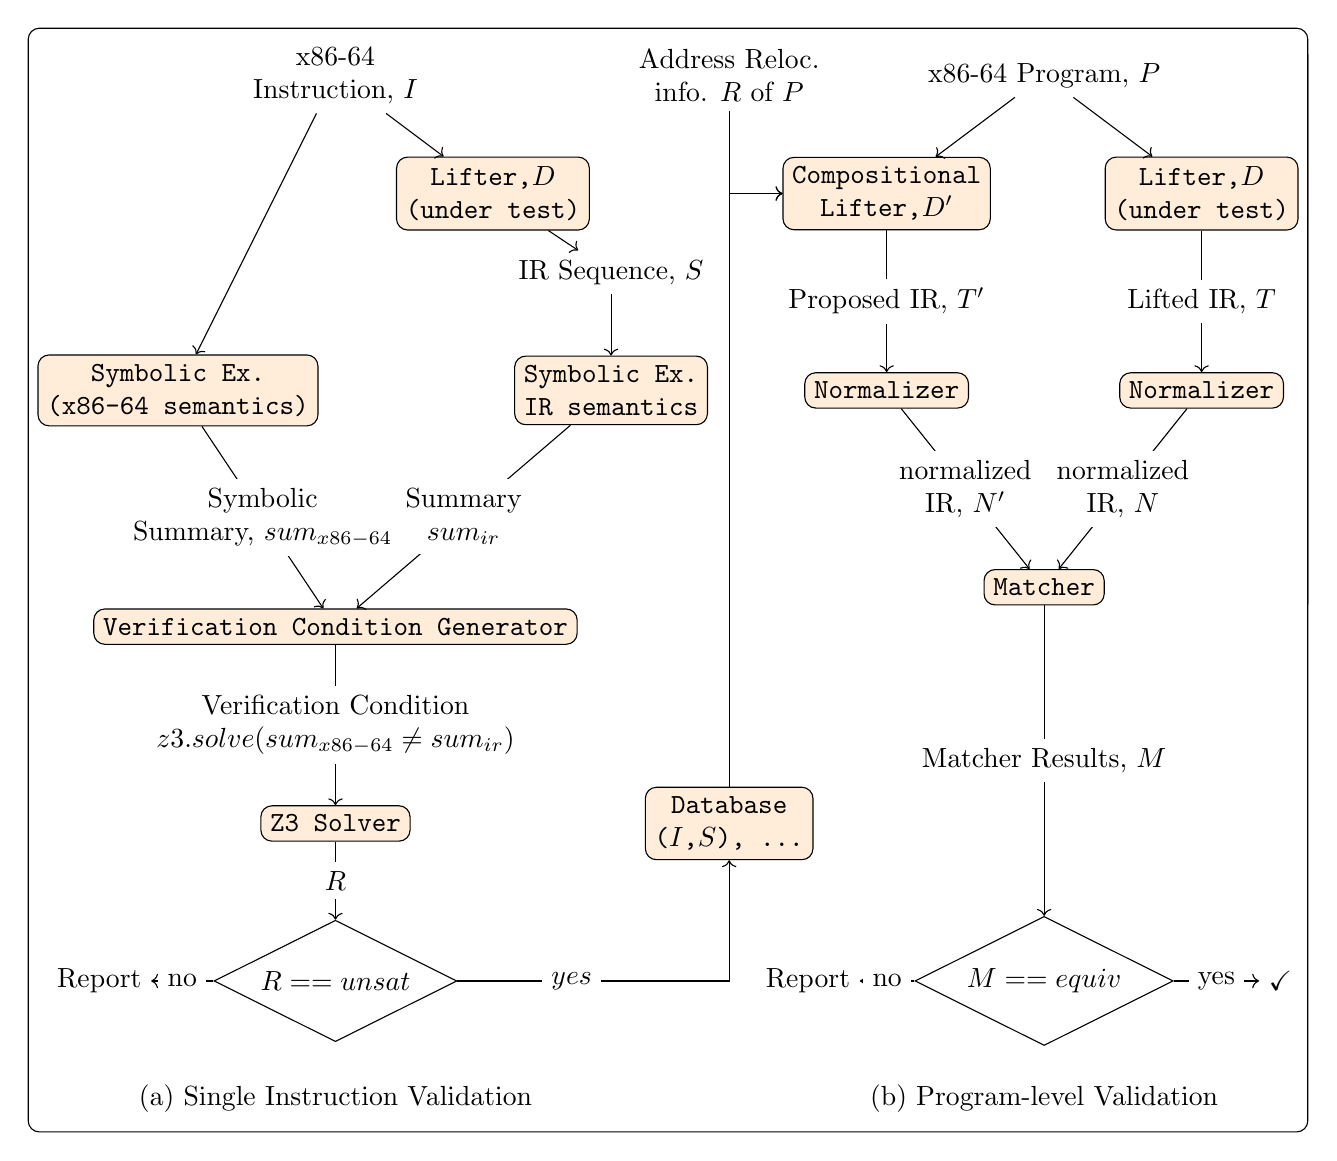
\begin{tikzpicture}[%node distance=2.5cm,
every node/.style={fill=white}, align=center]
\tikzset{%
    %>={Latex[width=2mm,length=2mm]},
    % Specifications for style of nodes:
    base/.style = {rectangle, rounded corners,
         text centered},
    process/.style = {base,  fill=orange!15, font=\ttfamily, draw=black},
    basic box/.style = {
        shape = rectangle,
        align = center,
        draw  = #1,
        %fill  = #1!25,
        rounded corners},
      header node/.style = {
        %Minimum Width = header nodes,
        font          = \strut\Large\ttfamily,
        text depth    = +0pt,
        fill          = white,
        draw},
      header/.style = {%
        inner ysep = +1.5em,
        append after command = {
            \pgfextra{\let\TikZlastnode\tikzlastnode}
            node [header node] (header-\TikZlastnode) at (\TikZlastnode.north) {#1}
            %node [span = (\TikZlastnode)(header-\TikZlastnode)] at (fit bounding box) (h-\TikZlastnode) {}
        }
      },
}
\def\blockhdist{2cm}
\def\blockvdist{1.5cm}
\def\phasehdist{8cm}

%%%%%%%%%%%%%%% PHASE I
\node (instr)          [base]  {\ISA\\ Instruction, $I$};
\node (SIVmcsema)   [process, below of=instr, yshift=-0.5cm, 
xshift=\blockhdist]  {Lifter,$D$\\(under test)};
\node (irseq)          [base,below of=SIVmcsema, xshift=\blockvdist]  {IR 
Sequence, $S$};
\node (instrSymEx)   [process, below of=instr, yshift=-2*\blockvdist, xshift=-\blockhdist] {Symbolic Ex.\\(\ISA semantics) };
\node (irSymEx)   [process, below of=irseq, yshift=-0.5cm] {Symbolic Ex.\\IR semantics};
\node (proofGen)   [process, below of=instr, yshift=-4*\blockvdist] 
{Verification Condition Generator};
\node (solver)   [process, below of=proofGen, yshift=-\blockvdist] {Z3 Solver};
\node (decide1)     [draw, below of=solver, yshift=-1cm, diamond, aspect=2]  {$R == unsat$};
\node (report1)       [left of=decide1, xshift=-\phasehdist/4]  {Report};
\node (caption1)     [below of=solver, yshift=-2.5cm] {(a) Single Instruction
    Validation};

\draw[->]             (instr) -- (SIVmcsema);
\draw[->]             (SIVmcsema) -- (irseq);
\draw[->]     (instr) -- (instrSymEx);
\draw[->]     (irseq) -- (irSymEx);
\draw[->]     (instrSymEx) -- node {Symbolic\\Summary, $sum_{\ISA}$} (proofGen);
\draw[->]     (irSymEx) -- node {Summary\\$sum_{ir}$ } (proofGen);
\draw[->]     (proofGen) -- node {Verification Condition\\$z3.solve(sum_{\ISA} 
\ne 
sum_{ir})$} (solver);
\draw[->]     (solver.south) -- node {$R$} (decide1.north);
\draw[->]     (decide1.west) -- node {no} (report1);

%%%%%% Store
\node (store)     [process, right of=solver, 
xshift=\phasehdist/2]{Database\\({$I$,$S$}), \dots};
\draw[->]       (decide1.east) -| node[xshift=-2cm] {$yes$} (store.south);


%%%%%%%%%%%% PHASE II
\node (start)             [base,right of=instr, 
xshift=\phasehdist]                       {\ISA Program, $P$};
\node (compd)             [process, below of=start, yshift=-0.5cm, 
xshift=-\blockhdist]          {Compositional\\Lifter,$D^\prime$};
\node (mcsema)             [process, below of=start, yshift=-0.5cm, 
xshift=\blockhdist]          {Lifter,$D$\\(under test)};
\node (normalizer1)             [process, below of=compd, yshift=-\blockvdist]   {Normalizer};
\node (normalizer2)         [process, below of=mcsema, yshift=-\blockvdist]   {Normalizer};
\node (matcher)     [process, below of=normalizer2, yshift=-\blockvdist, 
xshift=-\blockhdist]   {Matcher};
\node (decide2)     at (decide1 -| matcher) [draw,  diamond, aspect=2]  {$M == equiv$};
\node (caption2)     at (caption1 -| matcher) {(b) Program-level Validation};
\node (report2)       [left of=decide2, xshift=-\phasehdist/4]  {Report};
\node (fine)       [right of=decide2, xshift=\phasehdist/4]  {\checkmark}; 
 
\draw[->]             (start) -- (compd);
\draw[->]             (start) -- (mcsema);
\draw[->]     (compd) -- node {Proposed IR, $T^\prime$} (normalizer1);
\draw[->]     (mcsema) -- node {Lifted IR, $T$} (normalizer2);
\draw[->]     (normalizer1) -- node {normalized\\IR, $N^\prime$} (matcher);
\draw[->]     (normalizer2) -- node {normalized\\IR, $N$} (matcher);
\draw[->]     (matcher) -- node {Matcher Results, $M$} (decide2);
\draw[->]     (store.north) |-  (compd.west);
\draw[->]     (decide2.west) -- node {no} (report2);
\draw[->]     (decide2.east) -- node {yes} (fine);

%% Reloc info
\node (reloc)             [base,right of=instr, 
xshift=\phasehdist/2]                       {Address Reloc. \\ info. 
$R$ of $P$};
\draw[->]       (reloc.south) |-  (compd.west);

%% Outter box
\begin{scope}[on background layer]
\node[fit = (compd)(mcsema)(start)(matcher), basic box = black,] (Phase1) {};
    \node[fit = (compd)(mcsema)(start)(matcher)(instr)(solver)(irseq)(instrSymEx)(irSymEx)(caption1)(caption2), basic box = black,] (Overview) {};
\end{scope}

\end{tikzpicture}
\caption{Overview diagram of the \tv framework}\label{fig:overview}
\end{figure*}

% \tikzset{
%     database/.style={
%         path picture={
%             \draw (0, 1.5*\database@segmentheight) circle [x radius=\database@radius,y radius=\database@aspectratio*\database@radius];
%             \draw (-\database@radius, 0.5*\database@segmentheight) arc [start angle=180,end angle=360,x radius=\database@radius, y radius=\database@aspectratio*\database@radius];
%             \draw (-\database@radius,-0.5*\database@segmentheight) arc [start angle=180,end angle=360,x radius=\database@radius, y radius=\database@aspectratio*\database@radius];
%             \draw (-\database@radius,1.5*\database@segmentheight) -- ++(0,-3*\database@segmentheight) arc [start angle=180,end angle=360,x radius=\database@radius, y radius=\database@aspectratio*\database@radius] -- ++(0,3*\database@segmentheight);
%         },
%         minimum width=2*\database@radius + \pgflinewidth,
%         minimum height=3*\database@segmentheight + 2*\database@aspectratio*\database@radius + \pgflinewidth,
%     },
%     database segment height/.store in=\database@segmentheight,
%     database radius/.store in=\database@radius,
%     database aspect ratio/.store in=\database@aspectratio,
%     database segment height=0.1cm,
%     database radius=0.25cm,
%     database aspect ratio=0.35,
% }


\section{Single \ISA Instruction Validation}
\section{Preliminaries}
\label{sec:prelim}

In this section, we provide background on various pieces of our work:
(i) The binary lifter under test, McSema, (ii) The formal \ISA semantics, and
(iii) The formal \LLVM semantics.

\paragraph{McSema}\label{par:mcsema} \mcsema~\cite{McSema:Recon14} is the most
mature, well tested, open-source lifter to raise binaries from \ISA
instructions to LLVM bitcode.  At a high-level, \mcsema is split into two
parts: (a) frontend, and (b) backend. The frontend is responsible for parsing,
loading, and disassembling a binary and exports an interface to the backend to
query for the required information, e.g., the defined symbols, sizes of
various binary sections, instruction listings etc. The backend then uses this
information and Remill~\cite{Remill} library to lift the individual
instructions. McSema supports multiple different frontends with IDA Pro being
the most robust, and supported option.

Conceptually, the backend implementation of \mcsema is fairly straightforward:
\mcsema exposes all of architecture state, i.e., the program registers,
conditional flags, and program memory, through an LLVM \emph{struct}, aptly
named \Mcstate. 
Member fields
of the structure correspond to every register (register name, not a physical
register) and flags that can be used during the execution of the program. Instructions
operating on the stack must retrieve the current top of stack from the
appropriate member field (corresponding to \reg{rsp}) in the structure.
\mcsema simply scans through the disassembly of the binary
and lifts each instruction one by one, emitting code to read and update the
members of \emph{state} as defined by the instruction semantics. In essence,
the code lifted by \mcsema simply \emph{simulates} the binary in \LLVM.

%The main idea behind \mcsema lies in the simulation of the original binary,
%which in turns requires architectural state and memory of the target
%processor. There is no explicit stack by default.  To simulate state of the
%processor, an LLVM structure type called \emph{state} is used. Member fields
%of the structure correspond to every register (register name, not a physical
%register) that can be used during the execution of the program. Instructions
%operating on the stack must retrieve the current top of stack from the
%appropriate member field (corresponding to \reg{rsp}) in the structure.
%%\todo[inline]{Unclear: Since structure only holds registers, say which
%%register is used to retrieve "current top of stack."}
%\mcsema  performs decompilation of the binary code by translating the machine
%instructions to operations on this \emph{state} structure, according to the
%machine specification. This lifting process works by translating each assembly
%instruction in the procedure into an IR sequence,  which explicitly specifies
%how it affects the machine's memory and registers, including the flags.
%\paragraph{\ISA \& LLVM formal semantics}
%The present work needs the formal
%semantics of \ISA and LLVM, which we borrowed from~\cite{DasguptaAdve:PLDI19}
%and~\cite{LLVMSEMA} respectively. Both semantics are developed using
%\K~\cite{k-primer-2013-v32}\cmt{\url{http://kframework.org}}, which is a
%framework for defining formal language semantics.

\paragraph{K-Framework}\label{par:k} The presented work needs the formal
semantics of \ISA and LLVM, which we borrowed from~\cite{DasguptaAdve:PLDI19}
and~\cite{LLVMSEMA} respectively (and described next). Both semantics are developed using
\K~\cite{k-primer-2013-v32}\cmt{\url{http://kframework.org}}, which is a
framework for defining formal language semantics. Given a syntax and a
semantics of a language, \K automatically generates a parser, an interpreter, 
a symbolic execution engine, as well as
formal analysis tools such as model checkers and deductive program verifiers,
at no additional effort. Using the interpreter, one can test their
semantics immediately, which significantly increases the efficiency of
semantics developments. Furthermore, the formal analysis tools
facilitate formal reasoning about the given language semantics.  This
helps both the applicability of the semantics and in the
engineering the semantics itself.

\paragraph{\ISA Formal Semantics} Our work uses the state-of-the-art \ISA
semantics developed by Dasgupta et al.~\cite{DasguptaAdve:PLDI19}, which
presents the most complete and thoroughly tested formal semantics of x86-64 to
date, and faithfully formalizes all non-deprecated, sequential
user-level instructions of x86-64 Haswell instruction set architecture.
This totals to 3155 instruction variants, corresponding to 774 mnemonics.
Their semantics are fully executable, and includes a symbolic execution engine
automatically generated by \K framework
%
    \footnote{Given a syntax and a semantics of a language, \K automatically
    generates a parser, an interpreter, a symbolic execution engine, as well
    as formal analysis tools such as model checkers and deductive program
    verifiers, at no additional effort.}.
%

\paragraph{\LLVM Formal Semantics} We use the LLVM formal semantics as defined
in \K~\cite{LLVMSEMA}, which models LLVM types (integers, composite arrays and
structs, corresponding pointers), the \texttt{getelementptr} instruction (used
to compute the address of an element nested within a composite),  integer
arithmetic \& comparison operators, memory operations (\texttt{load},
\texttt{store}, and \texttt{alloca}), control flow instructions for
unconditional and conditional branches, as well as function calls and returns.
However, the semantics does not support: floating point, vector types, and
most LLVM intrinsic functions and therefore we cannot validate the \tv for
such instructions.  This is a limitation of the available LLVM semantics, and
not a limitation of our work.

.
%\todo[inline]{The last 2 sentences are nice, but could be dropped if space is tight.}
%\todo[color=yellow]{These two semantics are two of the most
%    important building blocks. Can we make them top-level paragraphs?}
%\paragraph{\ISA Semantics} \todo{These two semantics are two of the most
%important building blocks. Can we make them top-level paragraphs?}
%The formal model~\cite{DasguptaAdve:PLDI19}
%presents the most complete and thoroughly tested formal semantics of x86-64 to
%date, which faithfully formalizes all the  non-deprecated, sequential
%user-level instructions of the x86-64 Haswell instruction set architecture.
%This totals 3155 instruction variants, corresponding to 774 mnemonics.  The
%semantics is fully executable, and comes with an
%automatically generated symbolic execution engine (thanks to the \K framework),
%which we leverage in this work.
%
%\paragraph{LLVM Semantics} The formal semantics of \LLVM is provided by
%~\cite{LLVMSEMA}, which models  various LLVM types (like integer types,
%    composite array and struct types, the  corresponding pointer types, and the
%    \texttt{getelementptr} instruction used to compute the address of an element nested
%    within a composite type),  integer arithmetic \& comparison operators,
%  memory operations (like \texttt{load}, \texttt{store}, and \texttt{alloca}), 
%  control flow instructions
%  for unconditional and conditional branches, as well as function calls and
%  returns. The current version of the semantics does not support floating point
%  or vector types and most LLVM intrinsic functions, which constrains our experiments
%  but does not affect the overall approach proposed and evaluation in this work.
%  \todo{Check last sentence.}

%\paragraph{Stoke Libraries}\label{par:stoke} Stoke~\cite{Stoke2013} is a
%stochastic superoptimizer and program synthesizer for the x86-64 instruction
%set.  The project comes with many useful libraries to (1) query interesting
%properties of \ISA instructions (like type, size, inputs \& outputs etc.),
%(2) disassemble \ISA programs, and (3) analyze  \ISA programs to infer
%properties related to control- \& data-flow. We make use of these in our
%work.
%
%The rest of this paper is organized as follows: we discuss our \siv
%in~\ref{sec:siv}, and then move on to show how we use the validated sequences of
%IR instructions to construct a \emph{\compd} and use it to for \plv
%in~\ref{sec:plv}. Finally, we show the effectiveness of our developed techniques
%through our evaluation in~\ref{sec:eval}.

\section{\ISA Program-Level Validation}
\subsection{Compositional Decompiler}
\subsection{Normalizer}
\subsection{Matcher}

\section{Preliminaries}
\label{sec:prelim}

In this section, we provide background on various pieces of our work:
(i) The binary lifter under test, McSema, (ii) The formal \ISA semantics, and
(iii) The formal \LLVM semantics.

\paragraph{McSema}\label{par:mcsema} \mcsema~\cite{McSema:Recon14} is the most
mature, well tested, open-source lifter to raise binaries from \ISA
instructions to LLVM bitcode.  At a high-level, \mcsema is split into two
parts: (a) frontend, and (b) backend. The frontend is responsible for parsing,
loading, and disassembling a binary and exports an interface to the backend to
query for the required information, e.g., the defined symbols, sizes of
various binary sections, instruction listings etc. The backend then uses this
information and Remill~\cite{Remill} library to lift the individual
instructions. McSema supports multiple different frontends with IDA Pro being
the most robust, and supported option.

Conceptually, the backend implementation of \mcsema is fairly straightforward:
\mcsema exposes all of architecture state, i.e., the program registers,
conditional flags, and program memory, through an LLVM \emph{struct}, aptly
named \Mcstate. 
Member fields
of the structure correspond to every register (register name, not a physical
register) and flags that can be used during the execution of the program. Instructions
operating on the stack must retrieve the current top of stack from the
appropriate member field (corresponding to \reg{rsp}) in the structure.
\mcsema simply scans through the disassembly of the binary
and lifts each instruction one by one, emitting code to read and update the
members of \emph{state} as defined by the instruction semantics. In essence,
the code lifted by \mcsema simply \emph{simulates} the binary in \LLVM.

%The main idea behind \mcsema lies in the simulation of the original binary,
%which in turns requires architectural state and memory of the target
%processor. There is no explicit stack by default.  To simulate state of the
%processor, an LLVM structure type called \emph{state} is used. Member fields
%of the structure correspond to every register (register name, not a physical
%register) that can be used during the execution of the program. Instructions
%operating on the stack must retrieve the current top of stack from the
%appropriate member field (corresponding to \reg{rsp}) in the structure.
%%\todo[inline]{Unclear: Since structure only holds registers, say which
%%register is used to retrieve "current top of stack."}
%\mcsema  performs decompilation of the binary code by translating the machine
%instructions to operations on this \emph{state} structure, according to the
%machine specification. This lifting process works by translating each assembly
%instruction in the procedure into an IR sequence,  which explicitly specifies
%how it affects the machine's memory and registers, including the flags.
%\paragraph{\ISA \& LLVM formal semantics}
%The present work needs the formal
%semantics of \ISA and LLVM, which we borrowed from~\cite{DasguptaAdve:PLDI19}
%and~\cite{LLVMSEMA} respectively. Both semantics are developed using
%\K~\cite{k-primer-2013-v32}\cmt{\url{http://kframework.org}}, which is a
%framework for defining formal language semantics.

\paragraph{K-Framework}\label{par:k} The presented work needs the formal
semantics of \ISA and LLVM, which we borrowed from~\cite{DasguptaAdve:PLDI19}
and~\cite{LLVMSEMA} respectively (and described next). Both semantics are developed using
\K~\cite{k-primer-2013-v32}\cmt{\url{http://kframework.org}}, which is a
framework for defining formal language semantics. Given a syntax and a
semantics of a language, \K automatically generates a parser, an interpreter, 
a symbolic execution engine, as well as
formal analysis tools such as model checkers and deductive program verifiers,
at no additional effort. Using the interpreter, one can test their
semantics immediately, which significantly increases the efficiency of
semantics developments. Furthermore, the formal analysis tools
facilitate formal reasoning about the given language semantics.  This
helps both the applicability of the semantics and in the
engineering the semantics itself.

\paragraph{\ISA Formal Semantics} Our work uses the state-of-the-art \ISA
semantics developed by Dasgupta et al.~\cite{DasguptaAdve:PLDI19}, which
presents the most complete and thoroughly tested formal semantics of x86-64 to
date, and faithfully formalizes all non-deprecated, sequential
user-level instructions of x86-64 Haswell instruction set architecture.
This totals to 3155 instruction variants, corresponding to 774 mnemonics.
Their semantics are fully executable, and includes a symbolic execution engine
automatically generated by \K framework
%
    \footnote{Given a syntax and a semantics of a language, \K automatically
    generates a parser, an interpreter, a symbolic execution engine, as well
    as formal analysis tools such as model checkers and deductive program
    verifiers, at no additional effort.}.
%

\paragraph{\LLVM Formal Semantics} We use the LLVM formal semantics as defined
in \K~\cite{LLVMSEMA}, which models LLVM types (integers, composite arrays and
structs, corresponding pointers), the \texttt{getelementptr} instruction (used
to compute the address of an element nested within a composite),  integer
arithmetic \& comparison operators, memory operations (\texttt{load},
\texttt{store}, and \texttt{alloca}), control flow instructions for
unconditional and conditional branches, as well as function calls and returns.
However, the semantics does not support: floating point, vector types, and
most LLVM intrinsic functions and therefore we cannot validate the \tv for
such instructions.  This is a limitation of the available LLVM semantics, and
not a limitation of our work.

.
%\todo[inline]{The last 2 sentences are nice, but could be dropped if space is tight.}
%\todo[color=yellow]{These two semantics are two of the most
%    important building blocks. Can we make them top-level paragraphs?}
%\paragraph{\ISA Semantics} \todo{These two semantics are two of the most
%important building blocks. Can we make them top-level paragraphs?}
%The formal model~\cite{DasguptaAdve:PLDI19}
%presents the most complete and thoroughly tested formal semantics of x86-64 to
%date, which faithfully formalizes all the  non-deprecated, sequential
%user-level instructions of the x86-64 Haswell instruction set architecture.
%This totals 3155 instruction variants, corresponding to 774 mnemonics.  The
%semantics is fully executable, and comes with an
%automatically generated symbolic execution engine (thanks to the \K framework),
%which we leverage in this work.
%
%\paragraph{LLVM Semantics} The formal semantics of \LLVM is provided by
%~\cite{LLVMSEMA}, which models  various LLVM types (like integer types,
%    composite array and struct types, the  corresponding pointer types, and the
%    \texttt{getelementptr} instruction used to compute the address of an element nested
%    within a composite type),  integer arithmetic \& comparison operators,
%  memory operations (like \texttt{load}, \texttt{store}, and \texttt{alloca}), 
%  control flow instructions
%  for unconditional and conditional branches, as well as function calls and
%  returns. The current version of the semantics does not support floating point
%  or vector types and most LLVM intrinsic functions, which constrains our experiments
%  but does not affect the overall approach proposed and evaluation in this work.
%  \todo{Check last sentence.}

%\paragraph{Stoke Libraries}\label{par:stoke} Stoke~\cite{Stoke2013} is a
%stochastic superoptimizer and program synthesizer for the x86-64 instruction
%set.  The project comes with many useful libraries to (1) query interesting
%properties of \ISA instructions (like type, size, inputs \& outputs etc.),
%(2) disassemble \ISA programs, and (3) analyze  \ISA programs to infer
%properties related to control- \& data-flow. We make use of these in our
%work.
%
%The rest of this paper is organized as follows: we discuss our \siv
%in~\ref{sec:siv}, and then move on to show how we use the validated sequences of
%IR instructions to construct a \emph{\compd} and use it to for \plv
%in~\ref{sec:plv}. Finally, we show the effectiveness of our developed techniques
%through our evaluation in~\ref{sec:eval}.

\section{Single Instruction Validation}\label{sec:siv}

The \siv is responsible for validating the lifting (using McSema) of an \ISA 
instruction \s{I} to \LLVM sequence \s{S}. This is achieved by (1) 
%Identifying the input/output variables for \s{I} and \s{S} and 
Establishing variable correspondence between \s{I} and \s{S}, (2) Generating 
symbolic summaries 
individually for \s{I} and \s{S} for each output variable, (3) Generating 
verification conditions meant to establish semantic equivalence between the 
corresponding pair of summaries, and solving those using an SMT solver (\Z). 
Next, we describe each one of these steps.

\paragraph{(1) Establishing variable correspondence:}   
%First, we need to identify the input/output variables of an \ISA instruction 
%and the corresponding lifted IR sequence. For each \ISA instruction, this 
%information is ready accessible using Stoke libraries to determine what are 
%the 
%implicit and explicit 
%register/memory/flags which are read or written by the instruction.
``Variable correspondence'' between \s{I} and \s{S} refers to identifying the 
correspondence between the input/output variables of \s{I}\footnote{By 
input/output variables of an instruction we mean implicit and explicit 
    register/memory/flags which are read or written.} and the 
    virtual registers in 
\s{S}. As described in Section~\ref{par:mcsema}, \mcsema uses a \Mcstate 
structure to
model the architecture state, which holds all the simulated architectural
registers at different offsets of the structure.\footnote{Another decompiler,
  fcd~\cite{FCD}, also has the similar approach of modeling.
    Rev.Ng~\cite{DiFederico:CC2017} models the architecture registers as LLVM
    globals.}  Hence, the input and output variables in the context of
    \mcsema are particular \emph{struct} fields, identified by constant offsets.
%
 As an example, for an instruction \instr{adcq \%rax, \%rbx}, the input variables are
 \reg{cf}, \reg{rax} \& \reg{rbx}, and output variables are \reg{rbx}, \reg{cf},
 \reg{pf}, \reg{sf}, \reg{zf}, \reg{of} and \reg{af}. 
The following shows how
 these input/output registers are mapped to the \mcsema \Mcstate structure.

\begin{lstlisting}[style=KRULE]
// State structure type (irrelevant fields shown as ...)
%struct.State (*$\mapsto$*) type { %struct.ArchState, ..., 
    %struct.ArithFlags,..., ..., ..., %struct.GPR, ...}

// Pointers to simulated registers are accessed as below
getelementptr inbounds %struct.State, %struct.State* 
    %state, i64 0, i32 (*\textbf{m}*), i32 (*\textbf{n}*), i32 0, i32 0

// Mapping of various simulated registers to getelementptr offsets
    rax (*$\mapsto$*) m = 6  n = 1;  rbx (*$\mapsto$*) m = 6  n = 3
     cf (*$\mapsto$*) m = 1  n = 1;   pf (*$\mapsto$*) m = 1  n = 3
     af (*$\mapsto$*) m = 1  n = 5;   zf (*$\mapsto$*) m = 1  n = 7
     sf (*$\mapsto$*) m = 1  n = 9;   of (*$\mapsto$*) m = 1  n = 13
\end{lstlisting}

We use the above architectural state representation of \mcsema to infer the
``variable correspondence'' between the \ISA instruction and its corresponding
lifted IR sequence\footnote{Similar inference
    for fcd~\cite{FCD}. For Rev.Ng~\cite{DiFederico:CC2017}, ``variable
    correspondence''  refers to  mapping between the \ISA registers and the
    LLVM globals}.

\cmt{  
For \mcsema, the ``variable correspondence''  means identifying the one-on-one
mapping between the \ISA registers and the \emph{struct} offsets.
%
\footnote{Same
  with fcd~\cite{FCD}. For Rev.Ng~\cite{DiFederico:CC2017}, ``variable
    correspondence''  refers to  mapping between the \ISA registers and the
    LLVM globals},}
%
% which is a trivial task once the input/output variable are already identified.
%
%\todo[inline,color=yellow]{I think we should use "variable correspondence" to 
%mean the mapping
%of operands of I to operands of S for each I in the input program. The mapping 
%above 
%is an architectural state representation, not a variable correspondence.  Your 
%%%tools 
%use the knowledge of the
%latter to extract the former automatically for each I.  Need to add a brief 
%paragraph here to describe that.}

%One may very rightfully think that it may not be easy or scalable to look into 
%the 
%implementation details of an arbitrary decompiler to collect such information. 
%To avoid that we developed an automated tool which will collect the such 
%variable correspondence information. The idea is to feed carefully selected 
%\ISA instructions to the  
 
\paragraph{(2) Generating symbolic summaries:}
The \K framework takes the formal semantics of \ISA and \LLVM and generates 
symbolic execution engines automatically, which we leverage to do 
symbolic execution of an \ISA instruction and the corresponding lifted \LLVM sequence 
individually. Before symbolic execution, we assign symbolic values to the input 
variables to obtain a summary over those. For the running example of 
\instr{adcq, \%rax, \%rbx}, the following shows the symbolic summary for just the 
output register \reg{rbx}\footnote{All the values or
    addresses, stored in registers, memory or
    flags, are represented as bit-vectors which are depicted in
    this paper as $V_W$ and interpreted as a bit-vector of size $W$
    and value $V$.}. 

\vspace{45pt}
%\todo[inline,color=yellow]{Usual notation is with a footnote: $V_W$. You could 
%use footnotes
%in formatted text and use W.V in the listings.  W.V makes the listing
%below very cluttered, though: wish there was a better choice.}

%\begin{minipage}{\linewidth}
%\vspace{10pt}
\begin{lstlisting}[style=KRULE]
// VX_CF, VX_RAX and VX_RBX are the symbolic values
// assigned to input variables.
extract ( 
    add ( 
        (#if eq ( VX_CF(*$_1$*) , (*$1_1$*) ) #then 
            add ( concat ( 0(*$_1$*) , VX_RAX(*$_{64}$*) ) , 1(*$_{65}$*) ) 
        #else 
            concat ( 0(*$_1$*) , VX_RAX(*$_{64}$*) ) 
        #fi)
        , concat ( 0(*$_1$*) , VX_RBX(*$_{64}$*)) 
        ) 
    , 1 , 65 ) 
\end{lstlisting}
%\end{minipage}

Similar symbolic summaries will be obtained for
 every simulated register in the lifter IR sequence,
which is omitted for brevity.

%%
\cmt{and 
(3) The fact that x86-64 ISA is largely stable and changes slowly
over time, we can keep a database of \emph{most} of the (\ISA
instruction,
validated IR sequence) pairs computed offline, but one-time, and
the phase two, on the other hand, can use the database for
composition.  Some
instructions variants like immediate, memory and control-flow cannot
be stored before-hand because it is impractical to compute the IR
sequence for all possible constant values. In these case, the IR
sequence can either be generalized from similar instances already
populated in the database or generated afresh and validated on the fly.}

The \ISA ISA includes instructions with Repeat String Operation 
Prefix (e.g. \instr{rep}, \instr{repz} etc.) to repeat a string instruction the 
number of times specified in the 
count register or until the indicated condition by the prefix is no longer met.
That is, their specification involves a loop which the symbolic 
execution must handle. We address this by symbolically executing those 
instruction with symbolic input state and comparing the summaries (using 
solver checks) of any single $i^{th}$ iteration of the two loops. This suffices 
to establish equivalence between the two loops, by coinductive 
reasoning~\cite{bisimulations} and the fact that such loops are bounded by a 
constant thus must terminate.

%\todo{"Capturing core behaviors" is not enough for soundness: can we make
%    a stronger argument?}

% Although we can only see a limited number of 
%iterations, this is sound as a single symbolic iteration is enough to 
%correctly capture the core behaviors of such instructions.

% how is this diff from Meandiff
% Meandiff converts the ind. iR to UIR and then to z3 quesries.
% wheeras we use the correctby construction K symbolic ex for the purpose.

\paragraph{(3) Generating \& Solving the verification conditions:}

First, we convert the summaries written in \K builtin operators to SMTLIB 
expressions. Given two symbolic summaries sum$_{\ISA}^{rbx}$ and 
sum$_{ir}^{rbx}$ for output \ISA register \reg{rbx} and corresponding 
simulated register, we emit a  query 
%\begin{center}
%\begin{tabular}{c}
\begin{lstlisting}[style=KRULEWOBORDER]
            (assert (not (= sum(*$_{\ISA}^{rbx}$*) (*sum$_{ir}^{rbx}$*))))
\end{lstlisting}
%\end{tabular}
%\end{center}

Similar  queries are generated for all registers, memory and 
flags (for examples, refer to~\cite{Suppl}). Note that we
generate queries for all registers/flags, not just the
ones clobbered, because the registers and flags not modified by
the instruction should have equivalent summaries (which is the unmodified value
    of the input symbolic value).

The verification condition queries are then dispatched to the \Z solver. If any 
two summaries 
fail to match, we have found a bug in McSema.

%\paragraph{\TV of instructions accessing data sections}

%\paragraph{Dispatching queries to solver}
Note that, even though we are using solver checks during the first phase, this
should not hamper the scalability of our program validation pipeline for 
the following
reasons.
First, the instruction-level validation is done for each instruction. 
Thus its verification condition is much simpler than that of whole program-level 
validation.
Second, the validation result of each instruction can be reused 
within a program  or across different programs, thus the validation cost can be 
amortized, or, done offline. 

%(1) Instruction lifting is checked one at a time and hence the solver
%queries are simple, (2) Most \ISA instructions do not have loops
%in their semantics (and the few that do are converted to a loop-free form),
%and therefore checking their equivalence is much easier than
%checking program-level equivalence using heavy-weight equivalence checkers.

\section{Program-Level Validation}\label{sec:plv}
The goal of \plv is to validate the translation of the input \ISA program
\s{P} to the Mcsema-lifted \LLVM program \s{T}.  Towards that goal, the first step
is to construct an alternative program \s{T$^\prime$} generated using the \compd
(Section~\ref{sec:compd}), which are then compare for syntactic equivalence 
using (Section~\ref{sec:matcher}).
%\todo{the last part of this sentence is confusing.  do you mean syntactic 
%checking?}

\subsection{Compositional Lifter}\label{sec:compd}
The \compd is responsible for generating the proposed \LLVM \s{T$^\prime$} by
composing the validated McSema-lifted IR sequences of the constituent binary
instructions of the \ISA program \s{P}. Importantly, the \compd design 
(Algorithm~\ref{alg:compd}) is simple---and took us about 
three man-weeks to implement. 

\s{P} is disassembled (line 2) to
identify function boundaries, and to decode 
instructions.
%Identifying functions is
%important because the Matcher (Section~\ref{sec:matcher}) will work at
%function-level granularity\todo{SD:makes sense?  CF: unclear whether this was 
%%%fundamental or just a design choice}. 
\cmt{Moreover, the framework 
is
plug-and-play in
using disassemblers other than ObjDump (line 2), like Intel's  XED~\cite{xed}.}
If the disassembled instruction $I_{disass}$ is already in Store, then its
corresponding (validated) IR sequence is reused.
Otherwise $I_{disass}$
is assembled (line 6) and lifted (using \mcsema) to
generate an \LLVM sequence that will be validated using Phase 1. The validated IR 
sequences are then composed (line 17) following program order.

\begin{algorithm}
    \SetKwInOut{Input}{Inputs}
    \SetKwInOut{Output}{Output}
    %\TitleOfAlgo{How to write algorithms}
    %\underline{function Euclid} $(a,b)$\;
    \Input{ \\
     \textbf{P:} \ISA binary program. \\
     \textbf{Store:} Validated pairs (<\s{I}, \s{S}> ) of instruction \s{I}
        and
        lifted IR sequence
        \s{S}. (possibly empty) \\
     \textbf{R:} Address Relocation information of binary P.
    }
    \Output{Lifted IR Program \s{T$^\prime$}}
    \BlankLine
    $T^\prime \gets \phi$ \\
    $P_{disass} \gets$ ObjDump($P$) \\
    \ForEach{\textup{function} $F_{disass}$ \textup{in} $P_{disass}$}{%
    \ForEach{\textup{instruction} $I_{disass}$ \textup{in} $F_{disass}$}{%
        \uIf{$I_{disass}$ \textup{not in} Store}{%
            $I \gets$ Assembler($I_{disass}$) \\
            $S \gets$ McSema($I$) \\
            Perform \TV of $I$ and $S$ (Phase 1) \\
            \uIf{\textup{Validation successful}}{%
            Add $<I_{disass},S>$ to $Store$
            }
            \Else {
            Report Bug
            }

        }
        \Else {
            \textup{Extract} $S$ \textup{from} $Store$ \textup{for}
            $I_{disass}$ \\
        }
        $T^\prime \gets$ \textup{Compose($T^\prime, S, R$)}
    }
    }
    \KwRet{$T^\prime$}
    %\NoCaptionOfAlgo
    \caption{\textbf{Compositional Lifting}}\label{alg:compd}
\end{algorithm}

\paragraph{Single instruction validation of control-flow instructions (line
8)}\label{sec:sivcntrl}

The \siv strategy described in Section~\ref{sec:siv} cannot be applied naively  
to control flow instructions. This is because the instruction fed to \mcsema 
(line 7), for \siv, is obtained from the disassembled instruction \s{I$_{disass}$},
wherein the relative offsets of binary jump/call instructions are specified as labels. 
Hence, the binary instruction \s{I} which we obtain from assembling \s{I$_{disass}$} 
(line 6), without program context, has an incorrect relative offset, which gets 
propagated to the lifted IR \s{S}.

We get around this problem by symbolically executing \s{I} with 
symbolic values 
assigned to the current PC and label.
That way, we get symbolic
summaries agnostic of the actual (incorrect) value of the relative offset.
Similarly, we symbolically execute  lifted IR sequence by assigning symbolic
values to the virtual register holding the simulated relative offset.

%Translation validation of control-flow instructions like \instr{jmp label} and
%\instr{call label} w/o the program context is a bit tricky because the behavior
%of these instruction are not context-free. For example, the behavior of
%\instr{jz rel\_off}, which updates the PC value to either PC +
%sizeInBytesOf(\instr{jz rel\_off}) or PC + sizeInBytesOf(\instr{jz rel\_off}) +
%rel\_off, is based on the value of current PC value \cmt{and the rel\_off}
%which depends on the position of the instruction in the \emph{.text} section of
%binary.

\paragraph{The ``Compose'' step}
Below we describe the step ``Compose'' (line 17), responsible for
composing the IR sequences together, using a few example binary
instructions.
%\todo{say, at a high level, what is going on with compose?  E.g., ``At a 
%high-level, Compose concatenates the instructions that were validated in Phase 
%1, based on the program P.''}

The composed program is initially empty. Upon encountering a function label, we
append the following code to it\footnote{\emph{mem} is pointer to an opaque 
struct type which together with return type allows ordering of memory
    operations if required.}.

\begin{lstlisting}[style=LLVM]
define %struct.Mem* @composedFunc(%struct.State*, i64, 
        %struct.Mem* mem)  {}
\end{lstlisting}

For an instruction \instr{adcq \%rax, \%rbx}, \mcsema generates the following
IR sequence.

\begin{lstlisting}[style=LLVM]
define internal %struct.Mem* @ADCImpl(
    %struct.Mem*, %struct.State*, i64*, i64, i64) {
    ; Does adc computation and updates destination RBX
    ; and flags (omitted for brevity)
}

define %struct.Mem* @sub_adcq_rax_rbx(%struct.State*, 
        i64, %struct.Mem* ) {
 %RIP = getelementptr ... ; Compute simulated RIP address
 %RAX = getelementptr ... ; Compute simulated RAX address
 %RBX = getelementptr ... ; Compute simulated RBX address
 %VAL_RBX = load i64, i64* %RBX
 %VAL_RAX = load i64, i64* %RAX
 ; RIP update based on instruction size
 %VAL_RIP = load i64, i64* %RIP
 %UPDATED_RIP = add i64 %VAL_RIP, 3
 store i64 %UPDATED_RIP, i64* %RIP
 %retval = call %struct.Mem* @ADCImpl(
        %struct.Mem* %2, %struct.State* %0, i64* %RBX,
        i64 %VAL_RBX, i64 %VAL_RAX)
 ret %struct.Mem* %retval
}
\end{lstlisting}

The above IR sequence is then appended to the composed program as below.

\begin{lstlisting}[style=LLVM]
define %struct.Mem* @composedFunc(%struct.State*, 
        i64, %struct.Mem* mem)  {
    ; Code: adcq %rax, %rbx	
    %loadMem = load %struct.Mem*, %struct.Mem** %mem
    %retval = call %struct.Mem* @routine_adcq_rax_rbx(
        %struct.State* %0, %struct.Mem* %loadMem)
    store %struct.Mem* %call, %struct.Mem** %mem

    ret %struct.Mem* retval
}
; Definitions of called functions omitted for brevity
\end{lstlisting}

A similar composition happens for most instructions, the exceptions being the control-flow
data section-accessing instructions, which we elaborate on next.

\paragraph{Composing control-flow instructions} As mentioned previously, the
``labeled'' control-flow assembly instructions, when assembled without program
context, generate incorrect offsets which get propagated to the lifted IR.
We fix this IR by replacing said incorrect relative offsets with the correct
offsets.

For instance, when \mcsema lifts \instr{jne .L\_40087e} in isolation,
it generates the following IR sequence:
%\vspace{10pt}
\begin{lstlisting}[style=LLVM]
define %struct.Mem* @sub_jne_.L_40087e(%struct.State*, 
        i64, %struct.Mem* ) {
  %RIP = getelementptr ... ; Compute simulated RIP address
  %RIP_VAL = load i64, i64* %RIP
  ; Compute true target (using incorrect offset)
  %TARGET1 = add i64 %RIP_VAL, <incorrect_val>
  ; Compute fall-through target
  %TARGET2 = add i64 %RIP_VAL, <instr. size>
  %retval = call %struct.Mem* @JNEImpl(..., i64 %TARGET1, i64 %TARGET2)
  ret %struct.Mem* %retval
}
\end{lstlisting}

And the composed program with transformed IR looks like
\begin{lstlisting}[style=LLVM]
define %struct.Mem* @sub_jne_.L_40087e(%struct.State*, 
        i64, %struct.Mem*,
        i64 %(*\textbf{true\_tgt}*), i64 %(*\textbf{false\_tgt}*)) {
  %RIP = getelementptr ... ; Compute RIP address
  %RIP_VAL = load i64, i64* %RIP
  ; Transformed code
  %TARGET1 = add i64 %RIP_VAL,  %(*\textbf{true\_tgt}*)
  %TARGET2 = add i64 %RIP_VAL,  %(*\textbf{false\_tgt}*)
  ; Rest same as above
}

define %struct.Mem* @composedFunc( %struct.State*, 
        i64, %struct.Mem* mem)  {
  ; ... previously composed code ...
  ; Code: jne .L_40087e	 RIP: 400855	 Bytes: 6
  %loadMem = load %struct.Mem*, %struct.Mem** %mem
  %retval = call %struct.Mem* @routine_jne_.L_40087e(
        %struct.State* %0, %struct.Mem* %loadMem, 
        i64 (*\textbf{41}*), i64 (*\textbf{6}*))
  store %struct.Mem* %retval, %struct.Mem** %mem
  ret %struct.Mem* %retval
}
\end{lstlisting}

\paragraph{Composing data-section access instructions}
Instructions accessing the data section, like \instr{movq 0x602040, \%rdi}
with the first operand being an address, cannot be lifted correctly in
isolation (without program context) because \mcsema does not have sufficient information to to distinguish constant from address. 
\Siv can only validate the fact whether the constant
(which could potentially be an address) is correctly moved to the destination register. 
However, the problem is the \plv cannot use that lifting because the resulting 
composed IR \s{T$^\prime$}, with a constant moved to \reg{rdi}, will be   
different from the
one lifted by \mcsema \s{T}, with a global address moved to \reg{rdi}.
Upon normalization, two such IRs will be optimized differently by LLVM, leading to two syntactically 
divergent normalized forms, even when the initial programs were equal.

%Note that this will not pose any
%problem while \siv, as we can validate just the fact whether the constant
%(which could potentially be an address) is moved to the destination register.
%However, the \plv cannot use that lifting because the resulting composed IR
%\s{T$^\prime$}, with a constant moved to \reg{rdi}, will be different from the
%one lifted by \mcsema \s{T}, with a \dlifted global address moved to \reg{rdi}.
%Two such IRs upon normalization (Section~\ref{sec:normalizer}) using LLVM
%optimizer
%allows different optimization opportunities leading two syntactically divergent
%normalized forms.

To aid in testing, we compile binaries with options to retain auxiliary
information. To disambiguate between cases where a constant is a reference
into the data section (e.g., an \texttt{int*}) v/s a scalar (e.g., an
\texttt{int}), we use relocation information, denoted by \s{R} in
algorithm~\ref{alg:compd}.  We allow \mcsema to (incorrectly) lift such
instructions in isolation and then we course-correct the lifted IR by
consulting the binary's relocation information to determine if an immediate
operand should be considered as an address or constant --- every immediate
operand that is a reference has a corresponding entry in the relocation table.
Missing this entry would automatically mean that the immediate is a constant.

For example, the incorrect IR generated by \mcsema when lifting \instr{movq
0x602040, \%rdi} in isolation is:
\begin{lstlisting}[style=LLVM]
define %struct.Mem* @sub_movq_0x602040___rdi(
        %struct.State*, i64, %struct.Mem* ) {
    ...
    %retval = call %struct.Mem* @MOVImpl(
        %struct.Mem* %2, %struct.State* %0,
        ; data-section addr 0x602040
        ; lifted as a constant
        %i64* %RDI, i64 6299712)

    ret %struct.Mem* %retval
}
\end{lstlisting}

The address relocation information in the binary allows us to identify the address
and the following correct lifting:
\begin{lstlisting}[style=LLVM]
%G_0x602040_type = type <{ [8 x i8] }>
@G_0x602040= global %G_0x602040_type zeroinitializer
define %struct.Mem* @sub_movq_0x602040___rdi(
        %struct.State*, i64, %struct.Mem* ) {
    ...
    %retval = call %struct.Mem* @MOVImpl(
     %struct.Mem* %2, %struct.State* %0,
     %i64* %RDI,
     i64 ptrtoint( %G_0x602040_type* @G_0x602040 to i64))

    ret %struct.Mem* %retval
}
\end{lstlisting}

We reiterate that \compd only uses relocation information to strengthen the
generated golden reference, \s{T$^\prime$}, when such information is
available, e.g., during test or development time. This allows for a tighter
specification, allowing our technique to find bugs at testing that would 
otherwise
be missed. During use of \compd in the field to validate the lifting of
\mcsema on an unknown, blackbox binary, we do not require this additional
information, at the cost of potentially missing bugs described above. Note
that this is a fundamental limitation because \ISA semantics for an
instruction has no notion of types, and therefore \s{T$^\prime$}, which is
based on \ISA semantics, should allow for the ambiguity and cannot enforce
stricter type requirements. McSema on the other hand is never given this
additional information as it is expected to work in the field where relocation
information is rarely available, except in library code.

%\subsection{Normalizer}\label{sec:normalizer}

Algorithm~\ref{alg:NM} summaries the normalization and subsequent matching 
phase.
Due to the nature of the composition, the composed program  is 
very similar to the lifted program. We leverage this observation to establish 
semantic equivalence between the two 
programs using an iterative matching and pruning strategy, realized by a tool 
we develop called the \matcher. Failure of the  
\matcher should be interpreted as a \emph{potential} bug in the lifted program. 
%comparing (using \emph{Matcher}) 
%the \emph{canonical 
%representations} of the input programs
%generated using LLVM  \emph{O3} passes \& iterative pruning. 
%uisng an iterative strategy of matching the LLVM 03 assisted canonicalized 
%program and sbsequent pruning.
\newcommand\mycommfont[1]{\footnotesize\textcolor{blue}{#1}}
\SetCommentSty{mycommfont}
\begin{algorithm}
    \SetKwInOut{Input}{Inputs}
    \SetKwInOut{Output}{Output}
    \Input{
        \textbf{T:} \dlifted IR. \\
        \textbf{T$^\prime$:} \compd lifted IR.
    }
   \Output{\textbf{True} $\implies$   \textbf{T} \& \textbf{T$^\prime$} 
   semantically equivalent \\
   \textbf{False} $\implies$   \textbf{T} \& \textbf{T$^\prime$} \emph{may-be}
   non-equivalent
}


    \BlankLine
    
    \ForEach{\textup{corresponding function pair (\F,\FP) in 
        (\T, \TP)}}{%
        
        \If{\textup{!Matcher(\F, \FP)}}{%
            \tcp{\textup{A potential bug in McSema while lifting \s{F}}}
            \KwRet{false}  \\ 
        }
        
    }
    \KwRet{true}
    %\NoCaptionOfAlgo
    \caption{\textbf{Normalization \& Matching}}\label{alg:NM}
\end{algorithm}
%\Output{ 
%    \textf{True} $\implies$  \textbf{T} \& \textbf{T$^\prime$} semantically 
%    equivalent \\
%    False: \textbf{T} \& \textbf{T$^\prime$}  equivalent
%}



%two programs we are comparing (\s{T} \& \s{T$^\prime$}) start out being very
%similar:   
%% Why we need a normalizer
%There is no control-flow changes 
%
%\mcsema generally does not change control flow, and does not add or remove
%almost \emph{any} operations. However, it hoists the address computations of
%all the simulated registers (using \emph{getelelementptr}) in the \emph{entry}
%basic block so that the simulated instruction semantics does not have to
%compute them again. Whereas, the \compd recomputes those address at every
%instruction site.  
%%
%Our approach is to leverage this observation and to syntactically compare
%\emph{canonical representations} of the input programs.  We generate such
%representations using a tool we develop called a \emph{normalizer}.  Our
%normalizer is current implemented using LLVM  \emph{O3} passes to be applied to
%both \s{T} \& \s{T$^\prime$}.




%During the canonicalization step performed by the compiler, the strand (in our
%case a procedure with a single basic block) is repre- sented by a directed
%acyclic graph (DAG) which stores the expression. Even though comparing DAGs is
%possible, we wanted to simplify our representation to some kind of tex- tual
%form, allowing for fast and simple comparison. This is accomplished by using
%opt to output a linearized version of the computation’s DAG. To finalize the
%transformation which eliminates the origin and compilation choices made in the
%creation of the binary code, the final refinement to our representation is
%normalizing the strands. This is done by re- naming all symbols in the strand,
%i.e., its registers and tem- porary values, into sequentially named symbols.
%This step is crucial for cross-architecture comparison, as the names of the
%specific registers used in a given computation have nothing to do with its
%actual semantics, and are completely different between architectures.

\subsection{Matcher}\label{sec:matcher}
% How does the normalized outs look like
% Choice os SSA graph -> Why not conflow graph
% Why the matcher + Semantics Preserving Transformation is sufficient.
Algorithm~\ref{alg:NM} summarizes our overall strategy to check equivalence 
between the IRs generated by \mcsema (\T) and \compd (\TP). Due to the nature 
of the composition, \T \& \TP are structurally very similar. 
We leverage this observation to establish 
semantic equivalence between the two using a graph-isomorphism based 
algorithm assisted by 
normalization.  The algorithm is realized by a tool 
we develop called the \matcher. If the   
\matcher fails to match \T \& \TP, there is a \emph{potential} bug in the lifted program. 
%comparing (using \emph{Matcher}) 
%the \emph{canonical 
%representations} of the input programs
%generated using LLVM  \emph{O3} passes \& iterative pruning. 
%uisng an iterative strategy of matching the LLVM 03 assisted canonicalized 
%program and sbsequent pruning.
\newcommand\mycommfont[1]{\footnotesize\textcolor{blue}{#1}}
\SetCommentSty{mycommfont}
\begin{algorithm}
    \SetKwInOut{Input}{Inputs}
    \SetKwInOut{Output}{Output}
    \Input{
        \textbf{T:} \dlifted IR. \\
        \textbf{T$^\prime$:} \compd lifted IR.
    }
    \Output{\textbf{True} $\implies$   \textbf{T} \& \textbf{T$^\prime$} 
        semantically equivalent \\
        \textbf{False} $\implies$   \textbf{T} \& \textbf{T$^\prime$} 
        \emph{may-be}
        non-equivalent
    }
    
    
    \BlankLine
    
    \ForEach{\textup{corresponding function pair (\F,\FP) in 
            (\T, \TP)}}{%
        
        \If{\textup{!Matcher(\F, \FP)}}{%
            \tcp{\textup{A potential bug in McSema while lifting \s{F}}}
            \KwRet{false}  \\ 
        }
        
    }
    \KwRet{true}
    %\NoCaptionOfAlgo
    \caption{\textbf{Matcher Strategy}}\label{alg:NM}
\end{algorithm}

The matcher algorithm is based on the following key observations on input IR 
programs, \s{T} \& \Tp, informally stated:
%
(I) Both exhibit identical control-flow and identical sequences of memory allocation
and reference behaviors (because McSema does not modify control flow or memory operations
during lifting).
%
(II) The single-instruction validation step proves that a memory store 
(respectively, load) in \s{T} writes (resp., reads) the equivalent set of memory
locations as does the corresponding operation in \Tp.  This property holds for
each dynamic instance of the corresponding instructions.

%
%, and 
%(III) There is no alloca instruction in either \T or \TP. All the load 
%(store) 
%instructions are reading from 
%(writing to) the Mcsema \Mcstate fields. This makes sense because for each 
%input \ISA instruction, both \T \& \TP simulates its read or write behavior on 
%register/flags/memory which are all modeled as fields in the \Mcstate 
%structure.

%Two instructions (one from each input program) which should match, as per its 
%data-flow behavior, may not occur in  their respective matching basic blocks. 
%This 
%is because  As the two input program 
%are not exactly equal to begin with, the instruction can get reordered 
%differently,

These two observations motivate an intuitively simple graph isomorphism strategy for
proving the equivalence of \T and \Tp.
%
Let us name the normalized versions of the function pair, \F \& \FP, as \FN \& 
\FNP.
The Matcher algorithm works on data dependence graphs, \GN \& \GNP, generated  
from \FN \& \FNP. A vertex of the graph represents an 
LLVM instruction and an edge between two vertices captures SSA def-use  or   
memory 
dependence relations. Memory dependence edges, extracted from alias analysis 
results, appear between LLVM load and 
store instructions.
\cmt{There is a particular reason why we do not add 
control-flow edges: It is evident from \emph{\textbf{Ob II}} that the input 
programs \T \& \TP, being not exactly equal to begin with, can be normalized 
differently and there is no guarantee that two matching instructions will end 
up in matching basic blocks. }
%\cmt{We 
%call an 
%instruction in \s{N} \emph{matching exactly} with 
%an instruction in \s{N$^\prime$}  if the containing sub-graphs are 
%isomorphic.} 

\paragraph{Soundness of Equivalence via Graph Isomorphism}
%
We argue informally that isomorphism of \GN \& \GNP implies semantic equivalence of
the programs \s{T} and \Tp. We consider all of memory used in an execution as a single
``SSA variable,'' which gets renamed at every store operation in the program.  A store
modifies some (unknown) subset of the locations in memory, and a load reads some
(unknown) subset of the bytes.  Given two isomorphic graphs \GN and \GNP, consider a 
matching pair of nodes representing a store instruction \s{S} in \s{T} and the 
corresponding store \Sp in \Tp.  A key to the correctness argument, below, is that
single-instruction validation proves that, if the initial state of memory and registers
is identical before executing \s{S} and \Sp, then the final state of memory and registers
is also identical, i.e., the same bytes have been written into the corresponding memory
locations.  Similarly, a matching pair of load instructions transfers identical bytes
from memory to SSA registers in \s{T} and \Tp.
%
The correctness argument then works as follows:
%
\begin{enumerate}
  %
  \item A node \s{N} and corresponding node \Np are equivalent because of the 
  equivalence proof constructed by single-instruction validation (Section~\ref{sec:siv}).
  %
  \item An SSA edge \s{A} $\rightarrow$ \s{B} and corresponding edge 
  \Ap $\rightarrow$ \Bp carry identical bytes of data, because \s{A} is equivalent
  to \Ap and \s{B} is equivalent to \Bp, by (1), above.
  %
  \item A memory edge \s{S} $\rightarrow$ \s{L} representing a \emph{true} memory
  dependence (i.e., a store-to-load dependence) and corresponding edge \Sp $\rightarrow$
  \Lp carry identical bytes of data, because \s{S} and \Sp store identical bytes into
  identical memory locations, and \s{L} and \Lp read identical bytes from identical
  memory locations.  The argument for \emph{anti} and \emph{output} memory dependences
  is similar.
  %
\end{enumerate}

Note that the above argument is independent of the precision of any static analysis
used to identify memory dependences.  A highly imprecise analysis (e.g., one that
says every store-load or store-store pair may be aliased) might lead to a failure to
prove isomorphism between \s{T} and \Tp, but will not claim isomorphism if the two
programs are not equivalent.  In practice, we find in our experiments, described in 
Section~\ref{sec:eval}, that the memory dependence edges from such a highly imprecise
analysis do indeed reduce the success rate of the Matcher, but only by a small amount.
A more precise analysis may improve the success rate, reducing the number of false
negatives.

\paragraph{Checking Graph Isomorphism}
%
We build on a subgraph-isomorphism algorithm from Saltz 
et al.~\cite{Saltz2014}, named 
\emph{dual-simulation} (refer Algorithm~\ref{alg:DS}),  to check if both \GN \& \GNP are 
subgraph-isomorphic to each other. The algorithm, in general, first 
retrieves initial potential match sets, $\Phi$,  for each vertex in one 
graph based on semantic and/or neighborhood information in the other graph.
In our case, the initial potential match set for an instruction 
\IN in \GN contains all the instructions in \GNP which have the same 
instruction opcode. Also, if \IN has constant operands then its potential 
matches must share 
those.  
Then the algorithm iteratively prunes out elements from the 
potential match 
set of each vertex based on its parents/child relations until it reaches a 
fixed-point.
%
Therefore, nodes \s{A} and \Ap in \GN and \GNP will be marked as isomorphic if
they have identical (isomorphic) sets of predecessors and successors.
%
Two edges will be marked as isomorphic if their source and sink nodes are isomorphic.

\begin{algorithm}
    \SetKwInOut{Input}{Inputs}
    \SetKwInOut{Output}{Output}
    \Input{ \\
        \textbf{\GN:} data-dependence graph of \N. \\
        \textbf{\GNP:} data-dependence graph of  \NP.
    }
    \Output{Check if \textbf{\GN} \& \textbf{\GNP} are isomorphic}
    \BlankLine

    changed $\gets$ true \\
    \While{changed} { 
       changed $\gets$ false \\
       \For{\un $\gets$ \GN } {
           \For{ \up $\gets$ \GN.adj(\un)} {
               \potpup $\gets$ $\emptyset$ \\
               \For{ \vn $\gets$ \potu } {
                   \potvup $\gets$ \GN.adj(\vn) $\cap$ \potup \\
                   \If{\potvup = $\empty$} {
                       remove \vn from \potu \\
                       \If{\potu = $\emptyset$} {
                           \KwRet{$\emptyset$} \\
                       }
                       changed $\gets$ true \\
                   }
                   \potpup $\gets$ \potpup $\cap$ \potvup \\
               }
               \If{ \potpup = $\emptyset$} {
                   \KwRet{$\emptyset$} \\
               }
               \If{ \potpup is smaller than \potup} {
                   changed $\gets$ true \\
               }
               \potup $\gets$ \potup $\cap$ \potpup \\
           }
       }
   }
   \KwRet{$\emptyset$} \\
    %\NoCaptionOfAlgo
    \caption{\textbf{Dual Simulation}}\label{alg:DS}
\end{algorithm}

%\cmt{Then we augmented the algorithm to infer the basic-block 
%correspondence 
%on the fly and use that information to prune out the potential sets of store 
%instructions.}

%\paragraph{\textup{\GN} \& \textup{\GNP} are non-isomorphic} 
%This could happen because the input functions (\F \& \FP), being not exactly 
%equal to begin with (from Obs. II), undergo different 
%optimizations. 
%
%There is one significant difference in the code in \s{T} and \Tp.
%%
%In \T, the addresses computations, using 
%\emph{getelelementptr} (gep in short) instructions, of all the simulated 
%registers 
%and flags  
%are hoisted in the \emph{entry} basic block. \mcsema does this as an 
%optimization so that  the subsequent data-dependent  
%instructions does not have to compute them again. 
%Whereas, in \TP  addresses of relevant registers and/or flags are recomputed at 
%every instruction site.  The normalizer is quite effective at transforming the two
%code versions to be similar, so that the data dependence graphs are isomorphic.
%
%
%As a simple example, consider the code snippets of the normalized function pair 
%(\FN \& \FNP). \FN is generated by normalizing \F, wherein the  
%simulated register \& sub-register address computations  are hoisted in 
%\reg{entry} block and 
%re-used at use-site. Whereas, \FNP is generated from \FP where the 
%simulated address is re-computed 
%at every use-site. \F and \FP upon normalization undergo 
%different optimizations; One with better CSE (common subexpr. elim.) than 
%the other.   
%\begin{lstlisting}[style=LLVMWOBORDER]
%          (*\FN*)                            (*\FNP*)
%%entry:                           %entry:
%  %expr = gep ...                 %expr = gep 
%  %cl =  gep %expr ...            %cl =  gep %expr 
%  %rcx = gep %expr ...            %rcx =  gep ...   
%  ...                               ... 
%%somebb:                          %somebb:
%  store to %rcx                      store to %rcx
%  ...                                ...
%%otherbb:                         %otherbb:
%  store to %cl                       store to %cl  
%  ...                                ... 
%\end{lstlisting}
%Clearly, the  \FN \& \FNP are equivalent, yet the naive isomorphism based 
%matcher has to declare them as non-equivalent because the corresponding graphs 
%are
%not isomorphic with the node \reg{cmn\_expr} in \GN has two out-edges versus 1 
%edge in \GNP. However, the key insight is: the  subgraph with nodes 
%\reg{expr}, 
%\reg{cl} and \s{store \%cl} in \GNP shares no data-dependent edges with the 
%rest of the graph and is isomorphic with the corresponding subgraph in \GN. We 
%can prune both the subgraph from their respective parent graphs and the 
%residual graphs, upon re-normalization, have better opportunity to get 
%normalized to isomorphic graphs.
%
%Again, consider the code snippets below. 
%%As before, \F has the   
%%simulated address computation, hoisted  in \reg{entry}, re-used in all its 
%%use-site.  
%%Whereas, \FNP is generated from \FP where the simulated address is re-computed 
%%at every use-site. 
%\FP upon normalization undergo 
%partial-redundancy-elimination to make the computation of \s{rax} 
%\emph{available} in both the paths (\reg{b0} and \reg{b1}), but missed 
% the opportunity to eliminate the common-subexpression, despite of the fact 
% that \s{pre\_rax} has no data-dependence on ``some-code''.      
%
%\begin{lstlisting}[style=LLVMWOBORDER]
%         (*\FN*)                            (*\FNP*)
%%entry:                         %entry:
% %rax =  gep ...                 ...   
% ...
% br %some_cond, %b0, %b1         br %some_cond, %b0, %b1
%%b0:                           %b0:
%    .. some-code ..               .. some-code ..
%                                 pre_rax = gep ...
%    br %merge                    br %merge
%%b1:                           %b1: 
%    store to %rax                rax1 = gep ... 
%                                 store to %rax1   
%    ; ...                        ; ...
%    br %merge                    br %merge
%%merge:                        %merge: 
%    store to %rax                rax2 = (*$\phi$*) [rax1, %b1], 
%                                         [%pre_rax, %b0 ]
%                                 store to %rax2
%\end{lstlisting}
%As before, despite the equivalence of \FN \& \FNP, the naive 
%matcher will fail to proof graph-isomorphism, resulting in false alarm.
%However, if we find the sub-graphs corresponding to ``some-code'' on either 
%side are matching exactly, then we can follow  the pruning strategy as before, 
%followed by normalization, and converge to isomorphic graphs.
%
%With that insight, we design the following iterative matching and pruning 
%algorithm (Algorithm~\ref{alg:Match}).  
%\begin{algorithm}
%    \SetKwInOut{Input}{Inputs}
%    \SetKwInOut{Output}{Output}
%    \Input{ \\
%        \textbf{\F:} \dlifted function. \\
%        \textbf{\FP:} \compd lifted function.
%    }
%    \Output{Check if \textbf{\F} \& \textbf{\FP} are semantically 
%        equivalent}
%    \BlankLine
%        itr $\gets$ MaxIter \\
%        \While{\textup{itr != 0}} {
%            $\FN \gets \textup{llvm-opt -O3 } (\F)$ \\
%            $\FNP \gets \textup{llvm-opt -O3 } (\FP)$ \\
%            
%            \GN $\gets$  data-dependence graph of \FN \\
%            \GNP $\gets$ data-dependence graph of \FNP \\
%            
%            \If{\GN \& \GNP are isoporphic} {
%                \KwRet{true}
%            }
%            
%            $(\F, \FP) \gets \textup{Prune isoporphic subgraphs from \GN \& 
%            \GNP}$
%            \BlankLine
%            itr $\gets$ itr - 1 \\
%        }
%        \KwRet{false}         
%    %\NoCaptionOfAlgo
%    \caption{\textbf{Matcher}}\label{alg:Match}
%\end{algorithm}
%The Matcher algorithm, being agnostic of the normalization pass, tries to 
%recover missed optimization opportunities during normalization. This ensures 
%that there will be very less false alarms.

%\todo[inline]{The soundness problem that Vikram pointed out: Removing code
%    might introduce undefined behavior, which the later opt passes might abuse
%    and we might end up getting false positive or false negatives.}


 

\paragraph{Comparison with LLVM-MD \& Peggy}
At this point, it is important to differentiate our approach to establish 
equivalence between two \LLVM programs, using  normalization followed by 
matching, 
from some of the existing
approaches for validating LLVM IR-to-IR optimization
passes, e.g. LLVM-MD~\cite{Tristan:2011} and Peggy~\cite{Stepp:2011}, which, 
like our approach, move away from simulation proofs, and instead use graph 
isomorphism techniques to prove equivalence. 
Both build graphs of expressions for each program, 
transform the graphs via a series of ``expert-provided'' rewrite rules, and 
check for equality. The rewrite-rules mimic various compiler-IR optimizations 
and hence the technique is precise when the output program is an 
optimization of the input program and the optimizations are captured by the 
rewrite  rules. 

Compared to these approaches, our normalizer is simpler, requires no additional 
implementation effort, and re-uses off-the-shelf, well-tested compiler passes 
to reduce the two programs to syntactic equivalence. Nevertheless, the 
normalizer is still very effective as shown in our evaluations.

%In our case, \s{T} (the \dlifted program) and \s{T$^\prime$} (the \compd 
%lifted 
%program) are structurally separated by idioms which 
%might be beyond the capability of compiler optimization passes to match 
%%%syntactically.
%Encoding such idioms as rewrite rules would make the 
%approach tied to a specific lifter, which is something we avoided by 
%making the matcher iterative. \todo[inline]{too heavy-weight for our purpose}

%\paragraph{Semantics Preserving Transformation}




%Matching expressions with complex φ-nodes seems well within
%the reach of any SMTprover. Our preliminary experiments with Z3 suggest that
%it can easily handle the sort of equivalences we need to show. However, this
%seems like a very heavy-weight tool. One question in our minds is whether or
%not there is an effective tech- nique somewhere in the middle: more
%sophisticated than syntactic matching, but short of a full SMT prover.
%\begin{lstlisting}[style=LLVMWOBORDER]
%          (*\F*)                            (*\FN*)
%%entry:                                 %entry:
% ; chain of geps to step                  %comon_expr = gep ...    
% ; thr. nested State struct               %cl =  gep %common_expr  
% ; to compute address of cl               %rcx = gep %common_expr
% %cl =  gep ...                           ...
%
% ; chain of geps to step
% ; thr. nested State struct
% ; to compute address of rcx 
% %rcx =  gep ...  
% ...
%%somebb:                                %somebb:
% store to %rcx                            store to %rcx                        
% ...                                      ...  
%%otherbb:                               %otherbb:   
% store to %cl                             store to %cl
% ...                                      ... 
%\end{lstlisting}
%Next,  looks at the code snippets of \FP and its normalized version \FNP.
%\begin{lstlisting}[style=LLVMWOBORDER]
%          (*\FP*)                            (*\FNP*)
%%entry:                                 %entry:
%                                          %common_expr = gep ...
%                                          %cl =  gep ... 
%                                          %rcx =  gep ... 
% ...                                      ...
%%somebb:                                %somebb:
% ; chain of geps            
% %cl =  gep ...
% store to %rcx                            store to %rcx                        
% ...                                      ...  
%%otherbb:                               %otherbb:   
% ; chain of geps
% %rcx =  gep ...  
% store to %cl                             store to %cl
% ...                                      ... 
%\end{lstlisting}


\section{Evaluation} \label{sec:Eval}

\paragraph{Instruction Level Validation}

\subparagraph{Results}

\subparagraph{Inconsistencies Found} 

\paragraph{Program Level Validation}
\section{Discussion}\label{sec:discussion}

In this section we discuss some limitations of our work and avenues for future
work.

\paragraph{Incomplete LLVM Semantics} The \LLVM semantics~\cite{LLVMSEMA} is
currently under development and does not support all LLVM abstractions, e.g.,
vector and floating point types and their associated operations, and various
intrinsics functions at the time of implementation. This is a limitation of
existing semantics and we believe the verification of lifted instructions that
use such unsupported features will work out-of-the-box when semantics are
available.

\paragraph{Formally Verified Normalizer} Our current implementation of the
normalizer uses a small number (of 15) LLVM passes to improve syntactic
matching between the McSema generated \s{T} and \s{T$^\prime$} proposed by
\compd. To prove soundness, these passes need to be formally verified to
perform only semantic preserving transformations. An alternative, more
promising approach is to develop simple graph transformations on SSA graphs to
mimic the transformations of LLVM passes and formally prove the
transformations preserve program semantics. We leave this to future work.

\paragraph{Extending to Other Lifters} Our current work focuses on McSema, the
most mature, open-source, binary to LLVM IR lifter. However, there are a
plethora of other lifters that are not formally verified. Extending our work
to support these systems is important for two reasons: (i) improving the
trust in binary lifters, and (ii) the improvements made to our system would
make it more generic enough for future binary lifters to get validation for
(nearly) free. We believe that this is mainly engineering effort that involves
customization of \compd to capture the idiosyncrasies of various lifters.

%Following are our current limitations.
%\begin{itemize}
    %\item 
    
    %\item The normalizer we are using is a heavyweight sequence of 
    %production compiler optimization passes. It is difficult to get confidence 
    %in their soundness, and hence the key weak link in the current approach.  
    %We are currently working to narrow down the list of optimizations we need 
    %to reduce the trust-base.  A more promising approach, for future,  would be 
    %to implement simpler  graph transformations on the SSA graphs being matched 
    %in order to mimic what the minimal LLVM passes do. We may even be able to 
    %write those as provably sound primitives using an interactive theorem 
    %prover, like Coq~\cite{Coq}.
    
    
%\end{itemize} 

\section{Related Work}\label{sec:RW}

% \Qt{Suggestion: I do not think we should include coverage numbers of projects that do not support direct semantics. And here are the reasons:
%     1. Projects like angr or mcsema do have support  of x87 or mmx which we do not have. That way if we include 
%     x87/mmx in the total instructions count we cannot say that we are 100\%.
%     2. Now if we exclude x87/mmx instructions and give the percentage (and that way we can say we are 100\%), but  that may confuse people. 
% 
%     We can include Strata and Goel's work in the table (or write in text ) and *can* include the percentages because neither of them support x87/mmx. For the others we can argue that they are not direct. Also we may 
%     add that bap, remill and radare2 are not complete. I can later will in what exact instruction they are missing  
%  }
% 
% \Qd{\revisit{I think we should ommit exact percentage numbers all together in the table. We should replace that column with a simple yes/no checkmark whether the semantics is complete. Also remove all together projects that do not give semantics directly to x86 but to some IL.}}

%There have been many projects that host a formal semantics of \ISA either as
%their main contribution or as part of their infrastructure.
%Table~\ref{table:RW} summarizes such previous work and compares it to our formal semantics.\footnote{Here we focus on comparing with other \emph{direct} semantics, since a complete \emph{direct} semantics is our goal and required for our purpose. We will discuss other \emph{indirect} semantics later in this section.}
%We do the comparison in three directions that reflect the
%primary contributions of our work: the completeness of the definition in terms
%of supported user-level instructions, the faithfulness of the definition in
%terms of whether it is executable and hence can be evaluated with real code
%execution, and the generality of the definition in terms of its applicability to
%formal reasoning analyses. Next, we discuss in more detail each of the
%related works.

There have been many projects that host a formal semantics of \ISA either as
their main contribution or as part of their infrastructure.
This section summarizes such previous work and compares it to our formal semantics based on three directions that reflect the primary contributions of our work: completeness, in terms of supported user-level instructions; faithfulness, in
terms of whether it is executable and hence can be evaluated with real code
execution; and generality, in terms of its applicability to
formal reasoning techniques.

\cmt{
\begin{table}
\scalebox{0.7}{
%\setlength{\arrayrulewidth}{.15em} 
\begin{tabular}{l||ccc}
\hline
\\ [-10pt]
\multicolumn{1}{l||}{\begin{tabular}[]{@{}c@{}}Project \\ Name\end{tabular}} & 
\multicolumn{1}{c}{\begin{tabular}[c]{@{}c@{}}Complete Support of \\ \ISA User-Level \\ Instructions (in scope) \end{tabular}} &
\multicolumn{1}{c}{\begin{tabular}[c]{@{}c@{}}Executable \\ Semantics\end{tabular}} &
\multicolumn{1}{c}{\begin{tabular}[c]{@{}c@{}}Support for \\ Full-Fledged \\ Formal Reasoning\end{tabular}} \\
\hline 
\\ [-10pt]
Strata~\cite{Heule2016a}          & \xmark & \rating{50} & \xmark      \\
Goel et al.~\cite{Goel:FMCAD14}  & \xmark & \cmark      & \cmark      \\
CompCert~\cite{Leroy:2009}        & \xmark & \cmark      & \cmark      \\
%Remill~\cite{Remill}              & \xmark & \cmark      & \xmark      \\
TSL~\cite{TSL:TOPLAS13}           & \xmark & \cmark      & \rating{50} \\
Sail ~\cite{sail-framework}        & \xmark & \cmark      & \cmark \\
Roessle \etal~\cite{Roessle:CPP19} & \xmark & \rating{50} & \cmark \\
\hline
\textbf{Our Semantics}            & \cmark & \cmark      & \cmark      \\
\hline
\end{tabular}}
\begin{center} 
{\small
    \cmark : Yes
    \quad
    \xmark : No % due to incorrect semantics
    \quad
    \rating{50} : Partially True
    \hfill
    %\quad
    %\emph{NJ}: Node.js 0.10.29
}
\end{center}
\caption{Projects hosting formal semantics of the \ISA ISA.}
\label{table:RW}
\end{table}
}

\Strata~\cite{Heule2016a} uses program synthesis to generate the instruction
semantics of X86-64 as SMT bit-vector formulas\cmt{, by learning their input/output behavior
through execution on an actual processor}. Automatically learning the formal semantics of 60\% of the target \ISA ISA
is impressive, and we leverage this result in our work.  However, the other 40\% of the
user-level instructions are not straightforward to automatically learn by their algorithm, mainly due to limitations of the underlying synthesis engine.  Moreover, the specifications are executable only for non-floating-point (FP) instructions.
%The FP operations are represented in the SMT formulas of the definition as
%uninterpreted functions. 
%Finally the specifications are given as SMT formulas but 
% have not been demonstrated to be usable in a formal analysis setting out-of-the-box.

\SC{A contemporary work by Roessle \etal~\cite{Roessle:CPP19} presents a method to extract the big step semantics of a binary program using the small step instruction semantics extracted mostly from Strata\footnote{There are some minor omissions on immediate instructions with $8$-bit operands for which Strata learns $256$ brute force formulas.} plus some manually drafted support for branching instructions and stack operations. Like Strata, their specification is executable only for the non-floating-point instructions. Moreover, their work does not aim for completeness of semantics, one of our primary goals.}

Goel \etal~\cite{Goel:FMCAD14} use the ACL2 theorem prover~\cite{ACL2:Kaufmann2000} to model the \ISA ISA and they support
\goelPerc{} of all user-level instructions~\cite{GoelList}, plus some system-level instructions, paging, and
segmentation.  This list is far from a complete semantic definition of \ISA,
but it is still the state-of-the-art in terms of formal analysis applied
directly to \ISA code. It is also an executable definition as demonstrated by
its use for simulations. In our work, we do not leverage this definition, since
\Strata has defined many more instructions.

The CompCert verified compiler~\cite{Leroy:2009} includes semantics
definitions for all intermediate and target languages used within the compiler,
including a definition for 32-bit x86 assembly. The definition is specified in Coq~\cite{Coq} and has been used in a formal
setting for proving the correctness of CompCert's compilation step to assembly,
as well as outside CompCert, e.g., in proofs relating to the certified concurrent
OS kernel CertiKOS~\cite{Gu:2016}. However, this definition focuses on the
32-bit x86 instruction set, which is a subset of the \ISA instruction 
set.
Moreover, it is part of the trust base for CompCert and it is not clear
whether or how it has been tested against an actual processor, whereas
\Strata and ours have been extensively tested.

TSL~\cite{TSL:TOPLAS13} is a system that can auto-generate tools for
various machine code analyses given a semantics definition of the machine
language written in the TSL specification. Such a semantics
definition for the integer instructions (i.e., no floating-point instructions) of the $32$-bit x86 instruction set is given
as part of the project. It is used to generate
various tools, including a machine code synthesizer~\cite{Srinivasan2015}.
This definition, to our knowledge, has not been used
for formal verification proofs, i.e., to prove whether a given x86
program meets its specification.

Our semantics, like all the other work cited above, uses a sequential consistency memory model, and not weaker memory models.
Existing efforts to specify weaker memory models for \ISA such as Owens et al.~\cite{Owens:x86-TSO} and Sarkar et al.~\cite{Sarkar:POPL09}, however, suffer from their limited support for instruction semantics (i.e., they consider only a small subset of 32-bit x86 instruction set).
We believe that integrating these two complementary efforts is a promising direction toward rigorously reasoning about real-world programs running on modern multiprocessors (e.g., using the Sail framework as we will describe below).

\SC{%
Sail is another language semantics framework, tailored for describing an instruction-set architecture semantics.  Sail has been used to specify the semantics of ARMv8-A, RISC-V, and CHERI-MIPS~\cite{sail-popl2019}, as well as the semantics of a small subset of x86~\cite{sail-x86}.  Sail is similar to the K framework we employed, but K is far more general-purpose than Sail.  Also, the Sail x86 semantics is much more limited than ours.  It describes the semantics of a fragment of 32-bit user-mode x86 instructions, while ours covers also the 64-bit counterpart as well as the floating-point instructions.
%
Sail, however, allows us to integrate a semantic definition with their relaxed memory models~\cite{rmem, Pulte:2017} for concurrency semantics.  We believe that (automatically) translating our semantics into Sail\footnote{Indeed, the Sail ARMv8-A semantics is automatically generated from the ARM-internal specification of ARMv8-A~\cite{Reid2017} written in the ARM's architecture specification language, ASL~\cite{asl}, by using the ASL-to-Sail translator~\cite{sail-popl2019}.} is a promising direction to obtain concurrency semantics and thus enable concurrency reasoning for x86 programs, which we leave as future work.
}

\SC{Overall, the key differentiator of our effort compared to the existing work, as cited above, is that our semantics achieves (A) completeness of supported  user-level instructions, (B) faithfulness, and (C) applicability to formal reasoning analyses. In Section~\ref{sec:lesson-learned}, we elaborate on our novel approaches that allow us to achieve this unique combination.}

There are various binary analysis projects that target \ISA binaries
and lift them to a higher-level representation more suitable for the
specific analysis. These include Angr~\cite{Angr} using the VEX IR of Valgrind~\cite{Valgrind:ENTCS03}, the QEMU~\cite{QEMU:USENIX05} emulator
using the TCG IR, the software fault isolation tool RockSalt~\cite{Roclsalt:PLDI12} using its own RTL DSL, the disassembler and binary analyzer Radare2~\cite{Radare2} using the ESIL IR~\cite{ESIL}, the binary analysis
tool BAP~\cite{BAP:CAV11} using the BIL IR, and  the static binary translator Remill~\cite{McSema:Recon14} using LLVM IR~\cite{LLVM:CGO04}.
We refer to these semantics as \emph{indirect} because they give the semantics of the \ISA binary via the translation to their IR, as opposed to a \emph{direct} semantics such as ours and the others cited earlier.
% because in all these cases the lifted IR, that is being analyzed, is rigorously defined as opposed to providing \emph{direct} semantics to the binary.
A direct semantics has significant advantages over an indirect semantics.
For example, without the direct semantics of \ISA, we cannot even formulate the correctness of a translator from \ISA to the IR.
Analogously, many programming languages (C, C++, Java, etc.) have been given direct semantics, instead of indirect semantics by translation to other languages, for formal reasoning at the desired language granularity. 

% Even though tools like BAP and Angr can do some formal reasoning owing to their capability of symbolically executing the IR semantics, but they are not designed with the goal of full-fledged formal reasoning.



\cmt{ 
Regarding the comparison with previous work, we focused on comparing with other direct semantics, since a complete *direct* semantics is our goal and required for our purpose.

In all these
cases the IR that is being analyzed is rigorously defined, but we refrain from
considering these as formal specifications of \ISA because the
actually specified language has abstracted away various features of \ISA.
For example, both VEX IR and RockSalt use different simplified register
semantics: VEX IR omits many implicit bit truncations
and/or extensions that are part of many \ISA instruction semantics 
(i.e., these have to be emulated separately by the program), while
RockSalt's DSL uses an infinite register file instead of the finite
\ISA register file.
}

Hasabnis \etal~\cite{Hasabnis:ASPLOS16, Hasabnis:FSE16} also present an indirect semantics of \ISA, but in contrast to other indirect semantics, they use machine learning~\cite{Hasabnis:ASPLOS16} and symbolic 
execution~\cite{Hasabnis:FSE16} to automatically learn the translation of \ISA instructions to their IR, by extracting knowledge from the hard-coded  translation logic of compilers such as GCC.
However, as they admitted~\cite{Hasabnis:FSE16}, their semantics omits some important details of \ISA semantics (e.g., the effect of various instructions on CPU flags), and thus is not sufficient to serve as a solid foundation for rigorous formal analyses of \ISA binary.

  
\cmt{ 
Remill~\cite{McSema:Recon14} is a static binary translator from \ISA to LLVM
IR~\cite{LLVM:CGO04}. The translator contains specifications for \ISA instructions
in the form of equivalent C\cmt{LLVM IR} programs to assist the translation. This
specification is neither complete nor formal and cannot be easily used
in formal analysis.
}


% implement
% lifting of \ISA to an architecture-independent intermediate language (IL).
% In contrast with the other works above,

% They learn these mappings by extracting
% knowledge from the hard-coded translation logic found in compilers such as GCC.
% The extracted mappings cover more than 99\% of \ISA instructions. However,
% \cmt{similar to the rest of binary analysis works,}
% the resulting IL cannot stand as a formal \ISA definition because it
% abstracts away important \ISA semantic details, e.g.,
% the effect of the various instructions on CPU flags.




%\section{Conclusion and Future Work}\label{sec:conc}
\section{Conclusion}\label{sec:conc}
We have presented the most complete formal semantics of \ISA user-level instructions
to date, and have thoroughly tested it using synthesized test inputs and the GCC torture tests.
%in different formal analyses such as symbolic execution, deductive verification, and translation validation.
We have also illustrated several potential uses of the semantics which are realized by the formal analysis tools
derived right from the \K specification. 
%Using the \K framework for our specification automatically provides several formal analysis tools from the specification, which greatly simplified these applications.
The \K framework also enables us to represent a semantics as SMT theories,
which other projects can
leverage for their own purposes.
%We describe several practical lessons we have learned from our experience in developing the semantics, which could be useful for future formal specifications of processor ISAs.


%As mentioned in Section~\ref{sec:Approach:Overview}, we found that our ideas of extending \Strata do not scale because we need information about the instructions, whose semantics we want to learn, in order to constraint the search space. This lesson suggested a new idea: the information needed to reduce the search space can be automatically extracted from the manual. This  information does not need to be precise, and we believe that such rough information can be automatically extracted from the manual using text processing.  We plan to explore this idea while defining the semantics of unspecified and/or new instructions.

%\SC{We plan to test our model against various x86-64 implementations (like AMD), which could uncover flaws in those implementations and/or additional imperfections in the manual.}

%\SC{Also, we aim to use our semantics for translation validation of the entire LLVM compiler back-end for X86-64, i.e., hundreds of thousands of lines of C++ code. Scalability is achieved by the modularity of the translation validation technique, where the verification of (small) sub-components are verified individually (hence can be massively parallelized) and their results are combined to obtain the final claim about the entire system.}

 

%\K  has success stories about defining the formal semantics of production languages like C~\cite{KC} and LLVM~\cite{KLLVM}. We can use that towards the benefit of binary lifters like ~\cite{McSema:Recon14, FCD} which lifts the binary code to LLVM IR for binary analysis and/or optimization. Having the semantics of both the source (\ISA) and the target language(LLVM) help in verifying the translation using symbolic reasoning and hence enhance trust in  the translation.

%\textit{Acknowledgements.}
%We warmly thank the \K team
%   for their technical support throughout the project.  Also we thank the Strata
%   developers for promptly confirming
%   our reported bugs and for answering all our questions in great detail.
   


\chapter{Ongoing and Future Work: Translator-agnostic Translation
  Validation}\label{sec:future}

With the overall goal of  establishing faithfulness of binary lifters, we
propose to use \tv to validate the translation from binary to LLVM IR\footnote{However, we believe that the core techniques are
    applicable to other decompilers targeting mid-level (language-neutral) IRs}. As
mentioned earlier, we employed \K framework as the formalism medium to
represent the source and target language and in the process, defined the most
complete semantics of user-level \ISA using the framework. We proposed to
borrow a language-independent equivalence checking algorithm
\m{Keq}~\cite{TheoSAS19} that can be parameterized with the input and output
language semantics. 
%The algorithm needs, as input, the \syncps for establishing equivalence
%between binary and LLVM IR programs, which can be generated by the translator
%itself.  .

As mentioned in Section~\ref{sec:approach}, the notion of equivalence between
binary program and the lifted LLVM IR is formalized as a bi-simulation
relation~\cite{Sangiorgi:2011} between pairs of states of the two programs.
These program points, also referred to as \syncps, are generated by a proof generator and fed to the equivalence
checker as inputs. There are various ways a proof generator can generate these
\syncps each having different challenges and trade-offs.

\section{Translator-specific approaches to SYNCHRONIZATION POINT
  generation}\label{sec:TS} One approach to generate the \syncps is by
  instrumenting the translator itself. 
%
% and can
%be generated, by a proof generator,  as hints by analyzing the translator
%itself. 
The translator, being aware of which high-level IR instructions and control
points are emitted for each binary instruction, can accurately generate the
\syncps. Moreover, each \syncp is labeled with invariants over symbolic
variables, corresponding to input/output program states, in order to cover only
observably equivalent states. For each \syncp, the equivalence-checker checks
equivalence by delegating proof obligations to an SMT solver. Failure of a
proof obligation can be attributed to either a bug in the translator or  the
fact that the source and target programs are not equivalent in the first place.
We can rule out the second possibility because the source and target programs
are not selected arbitrarily but they are the actual input and output of a
translator, under test, and hence claimed to be equivalent by the translator
itself.

However, the above approach requires modifications of the translator to
generate the \syncp points and hence it may not be easily scalable to other
decompilers. 

Another approach is to analyze the source (\ISA) code and target (LLVM IR) code
of a particular translation  and infer the synchronization points.
We note that the analyzer has to take into account translators specific idioms
while analyzing the target code because different binary translators might use
different ways to lift the binary code in the target IR. We would demonstrate
the applicability of this approach by validating the translation of a realistic
decompiler like McSema~\cite{McSema:Recon14}

\section{Translator-agnostic approaches to SYNCHRONIZATION POINT
  generation}\label{sec:TA}

The fact that the proof generator is using translator generated hints or idioms used by the translator
to  generate the \syncps \& the associated  invariants,  makes it  translator specific and hence not applicable
uniformly across translators. We aim for a  binary-translator-agnostic proof
generator, which, indeed, makes the problem  even more challenging. We would
like to explore the following  approaches towards that goal.

\paragraph{\textbf{Data-driven \syncp generation}} This approach
is based on inferring the \syncps using test-runs. There are two
notables~\cite{Iman2005,DDEC:OOPSLA:2013} along this direction which
deals with checking equivalence between GCC~\cite{GCC} RTLs or x86 loops respectively.

Iman \etal~\cite{Iman2005} proposed an algorithm for solving the problem of
finding basic block and variable correspondence between two GCC RTL programs
compiled from the same source, but using different optimizations.  The essence
of their technique is interpretation of the two programs on random inputs and
comparing the histories of value changes for variables.  If the sequences of
value changes of two variables are the same, then the variables probably
correspond to each other, and the block in which the changes occur might also
correspond to each other. However, the paper candidly admits that they do not consider  generation of
verification invariants (VCs) at a point of correspondence or proving the VCs, hence it is difficult
to judge  its effectiveness in proving the equivalence of the candidate RTL
programs.  \cmt{ Moreover, the paper do not try to address any reordering
  transformation, that is any transformation that changes the order of
    execution of code, without adding or deleting any executions of any
    statement. Also, using random values results in poor code coverage which is
    detrimental to finding variable correspondence. We note that only the basic
    blocks \m{b1} and \m{b2}, which are covered by the same test input run in
    original and optimized versions respectively, can be the candidate for
    correspondence.}   


%DDEC~\cite{DDEC:OOPSLA:2013} uses a combination of static analysis and
%data-driven inference for constructing simulation relations: Static analysis is
%used to determine the program locations of \syncps and the live
%variables while the constraints between variables are inferred from execution
%traces. 


Rahul \etal~\cite{DDEC:OOPSLA:2013} presented ``data-driven equivalence
checker'' (DDEC) to check equivalence of two x86 loops which uses data-driven
inference in order to guess candidate simulation relations\footnote{A 
  simulation relation can be roughly defined to consist of a pair of program cutpoints, which breaks two
    loops into a set of pairs of loop-free code fragments and  linear
    equalities as invariants to hold at those cutpoints.}. Their approach does
    not assume any knowledge about the optimization performed while determining
    those simulation relations. The candidate simulation relations are checked
    using an SMT solver to determine equivalence of the loops. The cutpoints
    are chosen where the corresponding memory states agree on the largest
    number of values. The equality conditions   at cutpoint is determined by
    using standard linear algebra techniques over the values of live variables
    recorded by inserting instrumentation. Moreover, DDEC is sound; a lack of
    test coverage may cause equivalence checking to fail, but it cannot result
    in the unsound conclusion that two loops are equivalent when they are not.
    \cmt{However, while DDEC is trying to prove that two x86 loops are
      equivalent, the proof obligation might fail because  of one or more of
        the following reasons: (1 ) If satisfactory cutpoints are not found,
            (2) If spurious equality relationships are produced as invariants,
            (3) There is a bug in the translator, and (4) The target and the
              rewrite are not equivalent in the first place. The attribution of
              failure reason seems non-trivial and could affect fully automatic
              application of the approach.}   

%Our proposed approach is based on the insight that a sound guess of
%synchronization points do not result in proving two programs equivalent when
%they are not (false positives). Indeed, they might produce false negatives.
%Having said that, 

Our proposed approach is based on the insight that
given  \ISA and translated LLVM programs, we might compile
the LLVM program to binary and use the data-driven
approach~\cite{DDEC:OOPSLA:2013}, mentioned above, to extract guesses of
\syncps. Next, we can map the \syncps back to the IR level and employ the equivalence
checker \m{Keq} to prove the equivalence of the resulting LLVM IR and the
original binary using the \syncp guesses. We note that, an incorrectly guessed, but sound \syncp will never result in proving two programs equivalent when
they are not (false positives) and hence we do not have to trust the compilation back-end.

%However, we do not want to add the compilation in our trust base and
%hence we can map the \syncps back to the IR level and employ the equivalence
%checker \m{Keq} to prove the equivalence of the resulting LLVM IR and the
%original binary using the \syncp guesses. 
However, these \syncp, being
data-driven guesses, may lead to failing the proof obligations for reasons
other than a translation error. For example, the proof might fail if the
spurious invariants are generated or the \syncps are not sufficient, and it is
highly non-trivial, but an interesting research problem, to automatically
attribute the failure reasons. 

There is a trade-off between translator-specific and translator-agnostic proof
generator approaches. The \syncps generated by the former is accurate, leading
to trivial and automatic attribution of proof failure reason. On the other
hand, the \syncp guesses produced by the  translator-agnostic proof generator
has issues with automatic attribution  of the failure reasons. We envision
opportunities to exploit this trade-off by pruning off \syncp  guesses which a
translator specific proof generator will never generate. For
  example, the equivalence checker \m{Keq}~\cite{TheoSAS19} is used for
    validating the compilation pipeline and it uses compiler generated hints to
    prove equivalence. The underlying algorithm mandates three
%equivalence-checker \m{Keq}~\cite{TheoSAS19}, which employs a
%translator-specific proof generator  to validate compilation,  dictates three
broad categories of synchronization points which are necessary and sufficient
to prove equivalence, viz., entry points, exiting points (which also include
    points before callsites), and the rest of the points (including loop entry
      points and points after callsites). We may use this information to prune
    redundant \syncp guesses generated by a translator-agnostic  proof
    generator like DDEC~\cite{DDEC:OOPSLA:2013}.

\paragraph{\textbf{Learning \syncps}}

As discussed in Section~\ref{sec:ml}, there exist many recent
efforts~\cite{Jaffe:2018ICPC,Rosenblum2007,Rosenblum:2008,Rosenblum:2010,Rosenblum:2011,Bao:2014,Shin:2015}
in extracting various features (like meaningful variable names, compiler
    provenance, function entry points) using machine learning techniques which
are useful for binary analysis. Most notable is the novel technique presented
by Katz \etal~\cite{katz2018rnn}  for decompiling binary code snippets using a
model based on Recurrent Neural Networks. The model learns properties and
patterns that occur in source code and uses them to produce decompilation
output. 
%

The employed model is  a sequence-to-sequence model based on RNNs. The model
composed of two recurrent neural networks: an encoder, which processes the
input binary sequence, and a decoder, which creates outputs, the decompiled C
code. Further, the sequence-to-sequence model contains a hidden state, which
summarizes the entire input sequence. 
%
The training input contains of a large pair of strings representing the snippet
of source C code and the corresponding binary output, derived from open source
projects.  The snippets are preprocessed  by tokenizing each string  and
translating the resulting token list to a list of integers. Preprocessing also
produces a dictionary to map which integers correspond to which tokens in both
the higher-level and binary snippets.  The encoder layer of the RNN is trained
using the list of integers, derived from binary and the decoder layer is
trained using the corresponding list of integers, derived from C code.  During
training, the encoder-decoder modifies its internal state and does not provide
additional output. For testing, the test-binary snippets are translated into
lists of integers, which is then fed to the trained encoder-decoder model to
output a list of integers, which  is later turned into  a predicted higher-level C
translation using the dictionary  generated in the preprocessing step.
%
There evaluation results suggest that the technique  can be used to obtain a high level
syntactic structure of the code.
    
    
For an input binary and the high-level IR, translated by an arbitrary
decompiler, our goal is to learn the corresponding \syncp. Using a
straightforward  supervised-learning approach, we could frame the problem as:
To predict if an arbitrary pair of program points is a \syncp or not?
Such a supervised-learning formulation requires providing  many input code
snippets, correctly labeled with \syncps, as the training set in the first
place. Indeed, it is interesting to explore how to harvest the input corpus. 
 

Another way of inferring the \syncps is by using ``Trial and Error'', for which
Reinforcement Learning~\cite{Sutton:1998} seems to be a better choice to
explore. For the ``Trial and Error'' approach to work, there must be an
efficient way to find the error state, namely, the tried \syncp is non-valid.
With that, the goal of inferring all the corresponding \syncps of an input
output program pair can be defined solely in terms of some \emph{reward} given
on each selection. For example, for each selection of \syncp, a \emph{reward}
can be assigned using the number of values on which the corresponding memory
states agree on, when they are both tested using a random set of same  inputs.

We believe such learning techniques are promising for this problem and we would like to explore more on this in the proposed work.



%%%%%%%%%%%%%%%%%%%%%%%%%%%%%%%%%%%%%%%%%%%%%%%%%%%%%%%%%%%%%%%%%%%%%%%%%%%%%%%
% APPENDIX
%
\appendix
%\include{apx}

\backmatter

%%%%%%%%%%%%%%%%%%%%%%%%%%%%%%%%%%%%%%%%%%%%%%%%%%%%%%%%%%%%%%%%%%%%%%%%%%%%%%%
% BIBLIOGRAPHY
%

\bibliographystyle{IEEE_ECE}
% Put references in BibTeX format in thesisrefs.bib.
\bibliography{bibs/references.bib,bibs/modeling-X86-semantics.bib,bibs/bugs.bib,bibs/k.bib,bibs/decompilaion-validation.bib}
%\bibliography{thesisrefs}


%%%%%%%%%%%%%%%%%%%%%%%%%%%%%%%%%%%%%%%%%%%%%%%%%%%%%%%%%%%%%%%%%%%%%%%%%%%%%%%
% AUTHOR'S BIOGRAPHY
% As of 10/03/2011, Author's Biography or Vita no longer accepted by Grad College

\end{document}
\endinput
